% ---------------------------------------------------------------------------
% Author guideline and sample document for EG publication using LaTeX2e input
% D.Fellner, v1.14, Nov. 29, 2017
\PassOptionsToPackage{table}{xcolor}
\documentclass{egpubl}
\usepackage{eurovis2019}

% --- for  Annual CONFERENCE
% \ConferenceSubmission   % uncomment for Conference submission
% \ConferencePaper        % uncomment for (final) Conference Paper
% \STAR                   % uncomment for STAR contribution
% \Tutorial               % uncomment for Tutorial contribution
% \ShortPresentation      % uncomment for (final) Short Conference Presentation
% \Areas                  % uncomment for Areas contribution
% \MedicalPrize           % uncomment for Medical Prize contribution
% \Education              % uncomment for Education contribution
% \Poster                 % uncomment for Poster contribution
% \DC                     % uncomment for Doctoral Consortium
%
% --- for  CGF Journal
% \JournalSubmission    % uncomment for submission to Computer Graphics Forum
% \JournalPaper         % uncomment for final version of Journal Paper
%
% --- for  CGF Journal: special issue
% \SpecialIssueSubmission    % uncomment for submission to , special issue
\SpecialIssuePaper         % uncomment for final version of Computer Graphics Forum, special issue
%                          % EuroVis, SGP, Rendering, PG
% --- for  EG Workshop Proceedings
% \WsSubmission      % uncomment for submission to EG Workshop
% \WsPaper           % uncomment for final version of EG Workshop contribution
% \WsSubmissionJoint % for joint events, for example ICAT-EGVE
% \WsPaperJoint      % for joint events, for example ICAT-EGVE
% \Expressive        % for SBIM, CAe, NPAR
% \DigitalHeritagePaper
% \PaperL2P          % for events EG only asks for License to Publish

% --- for EuroVis
% for full papers use \SpecialIssuePaper
% \STAREurovis   % for EuroVis additional material
% \EuroVisPoster % for EuroVis additional material
% \EuroVisShort  % for EuroVis additional material

%
 \electronicVersion % can be used both for the printed and electronic version

% !! *please* don't change anything above
% !! unless you REALLY know what you are doing
% ------------------------------------------------------------------------

% for including postscript figures
% mind: package option 'draft' will replace PS figure by a filname within a frame
\ifpdf \usepackage[pdftex]{graphicx} \pdfcompresslevel=9
\else \usepackage[dvips]{graphicx} \fi

\PrintedOrElectronic

% prepare for electronic version of your document
\usepackage{t1enc,dfadobe}

\usepackage{egweblnk}
\usepackage{cite}
\usepackage{balance}  % to better equalize the last page
\usepackage{graphics} % for EPS, load graphicx instead
\usepackage[T1]{fontenc}
\usepackage{txfonts}
\usepackage{mathptmx}
\usepackage[htt]{hyphenat}
% \usepackage[pdftex]{hyperref}

% \usepackage{booktabs}
% \usepackage{textcomp}
\usepackage{array}
\usepackage{booktabs}
\usepackage{pifont}
\usepackage{xspace}
\usepackage{setspace}
\usepackage{graphicx}
\usepackage{caption}
\usepackage[textsize=tiny]{todonotes}
% Some optional stuff you might like/need.
\usepackage{microtype} % Improved Tracking and Kerning
% \usepackage[all]{hypcap}  % Fixes bug in hyperref caption linking
\usepackage{ccicons}  % Cite your images correctly!
% \usepackage[utf8]{inputenc} % for a UTF8 editor only
\usepackage{verbatim}
\usepackage{relsize}
\usepackage{etoolbox}
\usepackage{lipsum}   % for filler text
\usepackage{setspace} % for \onehalfspacing and \singlespacing macros
\usepackage[normalem]{ulem}
\usepackage{enumitem}
\usepackage{relsize,etoolbox}% http://ctan.org/pkg/{relsize,etoolbox}
\usepackage{makecell}
\renewcommand\theadalign{bc}
\renewcommand\theadgape{\Gape[4pt]}
\renewcommand\cellgape{\Gape[4pt]}
\AtBeginEnvironment{quote}{\small}% Step font down one size relative to current font.

\def\plaintitle{You can't always sketch what you want: Understanding Sensemaking in Visual Query Systems}
\def\emptyauthor{}
\def\plainkeywords{Visual analytics, exploratory analysis, visual query}

\newenvironment{denselist}{
  \vspace{-5pt}
    \begin{list}{\small{$\bullet$}}%
    {\setlength{\itemsep}{0ex} \setlength{\topsep}{0ex}
    \setlength{\parsep}{0pt} \setlength{\itemindent}{0pt}
    \setlength{\leftmargin}{1.5em}
    \setlength{\partopsep}{0pt}}}%
    {\end{list}\vspace{-5pt}}
\newcommand{\squishlist}{
   \begin{list}{$\bullet$}
    { \setlength{\itemsep}{0pt}
      \setlength{\parsep}{2pt}
      \setlength{\topsep}{0pt}
      \setlength{\partopsep}{0pt}
      \leftmargin=25pt
\rightmargin=0pt
\labelsep=5pt
\labelwidth=10pt
\itemindent=0pt
\listparindent=0pt
\itemsep=\parsep
    }
}
\newcommand*{\img}[1]{%
    \raisebox{-.3\baselineskip}{%
        \includegraphics[
        height=\baselineskip,
        width=\baselineskip,
        keepaspectratio,
        ]{#1}%
    }%
}
\newcommand{\squishend}{\end{list}}
\newcommand{\npar}{\par\noindent}
% use extensively to toggle between paper and TR
\newcommand{\eat}[1]{}
% \newcommand{\papertext}[1]{{\leavevmode\color{blue}{#1}}}
% \newcommand{\techreport}[1]{{\leavevmode\color{red}{#1}}}
\newcommand{\papertext}[1]{#1}
\newcommand{\techreport}[1]{}
\newcommand{\nonannon}[1]{#1}
\newcommand{\annon}[1]{}
\newcommand{\boldpara}[1]{\par\noindent\textbf{#1}}
% de-facto paragraph format
\newcommand{\stitle}[1]{\noindent\textbf{#1}}
\newcommand{\nstitle}[1]{\\\noindent\textbf{#1}}
\newcommand{\cut}[1]{{\leavevmode\color{lightgray}{#1}}}
\newcommand{\ccut}[1]{} %confirmed cut

\newcommand{\problemlist}{
    \nstitle{Motivating Use Case Challenges:}
    \vspace{-5pt}
    \begin{enumerate}[label=\textbf{C\arabic*:},leftmargin=0.7cm]
}
\newcommand{\featurelist}{
    \stitle{Instantiated Feature:}
    \vspace{-5pt}
    \begin{enumerate}[label=\textbf{F\arabic*:},leftmargin=0.7cm]
}
\newcommand{\enumend}{
  \end{enumerate}
  \vspace{-5pt}
}
\urlstyle{leo}

% To make various LaTeX processors do the right thing with page size.
\def\pprw{8.5in}
\def\pprh{11in}
\special{papersize=\pprw,\pprh}
\setlength{\paperwidth}{\pprw}
\setlength{\paperheight}{\pprh}
\setlength{\pdfpagewidth}{\pprw}
\setlength{\pdfpageheight}{\pprh}

% create a shortcut to typeset table headings
% \newcommand\tabhead[1]{\small\textbf{#1}}
\newcommand{\zv}{\textit{zenvisage}\xspace}
\newcommand{\zvpp}{\textit{zenvisage++}\xspace}
\newcommand{\astro}{\textit{astro}\xspace}
\newcommand{\bio}{\textit{genetics}\xspace}
\newcommand{\matsci}{\textit{matsci}\xspace}
\newcommand{\change}[1]{\textcolor{red}{#1}}
\newcommand*\rot{\rotatebox{90}}

\newcommand{\agp}[1]{\textcolor{blue}{Aditya: #1}}
\newcommand{\dor}[1]{\textcolor{green}{Doris: #1}}
\newcommand{\kar}[1]{\textcolor{magenta}{Karrie: #1}}

\usepackage{xparse}   % http://ctan.org/pkg/xparse
% Rotation: \rot[<angle>][<width>]{<stuff>}
% \NewDocumentCommand{\rot}{O{320} O{2.2em} m}{\makebox[#2][r]{\rotatebox{#1}{#3}}}%
\newcommand*\OK{\ding{51}}
\renewenvironment{quote}{%
   \list{}{%
     \leftmargin0.15cm
     \rightmargin\leftmargin
   }
   \item\relax
}
{\endlist}
%%%%%%%%%%%%%%%%%%%%%%%%%%%%%%%%%%%%%%%%%%%%%%%%%%%%%%%%%%%%%%%%
%%%%%%%%%%%%%%%%%%%%%% START OF THE PAPER %%%%%%%%%%%%%%%%%%%%%%
%%%%%%%%%%%%%%%%%%%%%%%%%%%%%%%%%%%%%%%%%%%%%%%%%%%%%%%%%%%%%%%%%

\begin{document}
% \title{Understanding usage patterns for query specification in sketch-based visual query systems: A Case Study with Zenvisage}
%\title{I can't always sketch what I want: \\ Understanding Sensemaking in Visual Query Systems through Design Studies with Zenvisage++}
\title{\emph{You can't always sketch what you want}: \\ Understanding Sensemaking in Visual Query Systems \vspace{-50pt}}
%How are visual query systems used in practice?\\ A Design Study with Zenvisage}
\maketitle
\begin{abstract}
Visual query systems (VQSs) allow users to interactively search for line charts
with desired visual patterns typically specified using intuitive sketch-based interfaces. Despite their potential in accelerating data exploration, more than a decade of past work on VQSs has not been translated to adoption in practice. Through a year-long collaboration with experts from three diverse domains, we examine the role of VQSs in real data exploration workflows,  develop features to support these workflows by enhancing an existing VQS,
and evaluate how these features are used in practice. Via these observations, we formalize a taxonomy of key functionalities for VQSs, organized by three sensemaking processes. Perhaps somewhat surprisingly, we find that ad-hoc sketch-based querying is not commonly used during data exploration, since
analysts are \change{often unable} to precisely articulate the patterns they are interested in. We find that there is a spectrum of VQS-centric data exploration workflows, depending on the application, and that many of these workflows are not effectively supported in present-day VQSs. Our insights can pave the way for next-generation VQSs to be adopted in a variety of real-world applications.
% On characterizing the spectrum of workflows
% adopted,
% we find that there is
% Moreover, we find that there is a
% variety of typical workflows
% We offer guidelines for the next generation of
% VQSs

% We advocate that next-generation VQSs should support two other forms of sensemaking to pave way for these systems to be adopted to a variety of real-world applications.
% The increasing availability of rich and complex data in a variety of scientific domains poses a pressing need for tools to enable scientists to rapidly make sense of and gather insights from data. One proposed solution is to design visual query systems (VQSs) that allow scientists to interactively search for desired patterns in their datasets. While many existing VQSs promise to accelerate exploratory data analysis by facilitating this search, they are not widely used in practice. Through a year-long collaboration with scientists in three distinct domains---astronomy, genetics, and material science---we study the impact of various features within VQSs that can aid rapid visual data analysis, and how VQSs fit into scientists' analysis workflow. Our findings offer design guidelines for improving the usability and adoption of next-generation VQSs, paving the way for VQSs to be applied to a variety of scientific domains.
\end{abstract}
\keywords{Visual analytics, exploratory analysis, visual query}
\raggedbottom
%!TEX root=main.tex
\vspace{-5pt}
\section{Introduction\label{sec:intro}}
% one for each key finding: a) many features deemed to be of importance to VQSs by domain experts, not all supported by present-day VQSs b) sketch is inefficient, perhaps explaining why present-day VQSs are not popular c) identify 3 typical workflows involving various sensemaking modalities in different proportions, depending on the application
Line charts are commonly employed during data exploration---the
intuitive connected patterns
often illustrate complex underlying processes
and yield interpretable and visually compelling data-driven
narratives.
To discover patterns in line charts,
analysts construct them
using toolkits like \texttt{ggplot} or \texttt{matplotlib},
or visualization construction interfaces
like Excel or Tableau, specifying
{\em exactly} what they want to visualize.
For example, when trying to find celestial objects
corresponding to supernovae, which have a specific pattern
of brightness over time, astronomers
individually inspect the corresponding line chart
for each object (often numbering in the hundreds)
until they find ones that match the pattern. \ccut{Similarly, when trying to infer relationships between two physical properties for different subsets of battery electrolytes, scientists need to individually visualize these properties
for each subset (out of an unbounded number of such subsets)
until they identify relationships that make sense to them.}
This process of manual exploration of
large numbers of line charts
is not only error-prone, but also overwhelming for
analysts.
%, not only for time series but also for understanding the relationships between multiple measures variables.

% From high-throughput genome sequencing,
% to multi-resolution astronomical imaging telescopes,
% to at-scale physical testing of battery candidates,
% many fields of science and engineering
% are facing an increasing availability of
% large volumes of complex data~\cite{AustinNothaft2015,Demchenko2013},
% holding the key to some of the most pressing
% unanswered scientific questions of our time,
% such as: How does a treatment affect the
% expression of a gene in a breast cancer cell-line?
% Which battery components have sustainable levels
% of energy-efficiency and are safe and cheap to
% manufacture in production?
% While data analysis is central to a scientist's
% knowledge discovery process, scientists
% often lack the extensive experience to deal
% with data of this scale and complexity
% in a way that can facilitate rapid insight discovery~\cite{Kersten2011}.with the system automatically traversing all potential visualization candidates to find those that match the specification
\par To address this challenge,
there has been a large number of papers
dedicated to building {\em Visual Query Systems} (VQSs),
that allow users to specify
desired visual patterns
via an interactive interface~\cite{mohebbi2011google,Hochheiser2004,wattenberg2001sketching,Siddiqui2017VLDB,ryall2005querylines,correll2016semantics,Mannino2018,Eichmann2015,Holz2009}.
This interactive interface is one with
a sketching canvas
where users can draw a pattern of interest,
with the system automatically traversing
all potential visualization candidates
to find those that match the specification.
Since the intent of a sketch can be ambiguous,
some work has developed mechanisms to
enable users to clarify
how a sketch should be interpreted~\cite{ryall2005querylines,correll2016semantics,Mannino2018,Eichmann2015,Holz2009}.

\par
While this intuitive
specification interface
seems to be a promising solution
to the problem of painful manual exploration of visualizations,
to the best of our knowledge, VQSs are not very commonly used in practice.
{\em Our paper seeks to bridge this gap
to understand how VQSs can actually be used in practice,
as a first step towards the broad adoption of VQSs in data analysis}.
Unlike prior work on VQSs,
we set out to not only evaluate VQSs in-situ on
real problem domains, but also involve participants
from these domains in the VQS design.
We present findings from a series of interviews,
\change{contextual inquiry}, participatory design,
and user studies with scientists from three different domains---{\em astronomy, genetics,} and {\em material science}---over the course of
a year-long collaboration.
These domains were selected to capture
a diverse set of goals
and datasets wherein VQSs can help address
important scientific questions, such as:
How does a treatment affect the expression
of a gene in a breast cancer cell-line?
Which battery components have sustainable
levels of energy-efficiency and are safe and
cheap to manufacture in production?
\begin{figure*}[ht!]
	\centering
	\captionsetup{justification=centering,margin=2cm}
	\vspace{-10pt}
	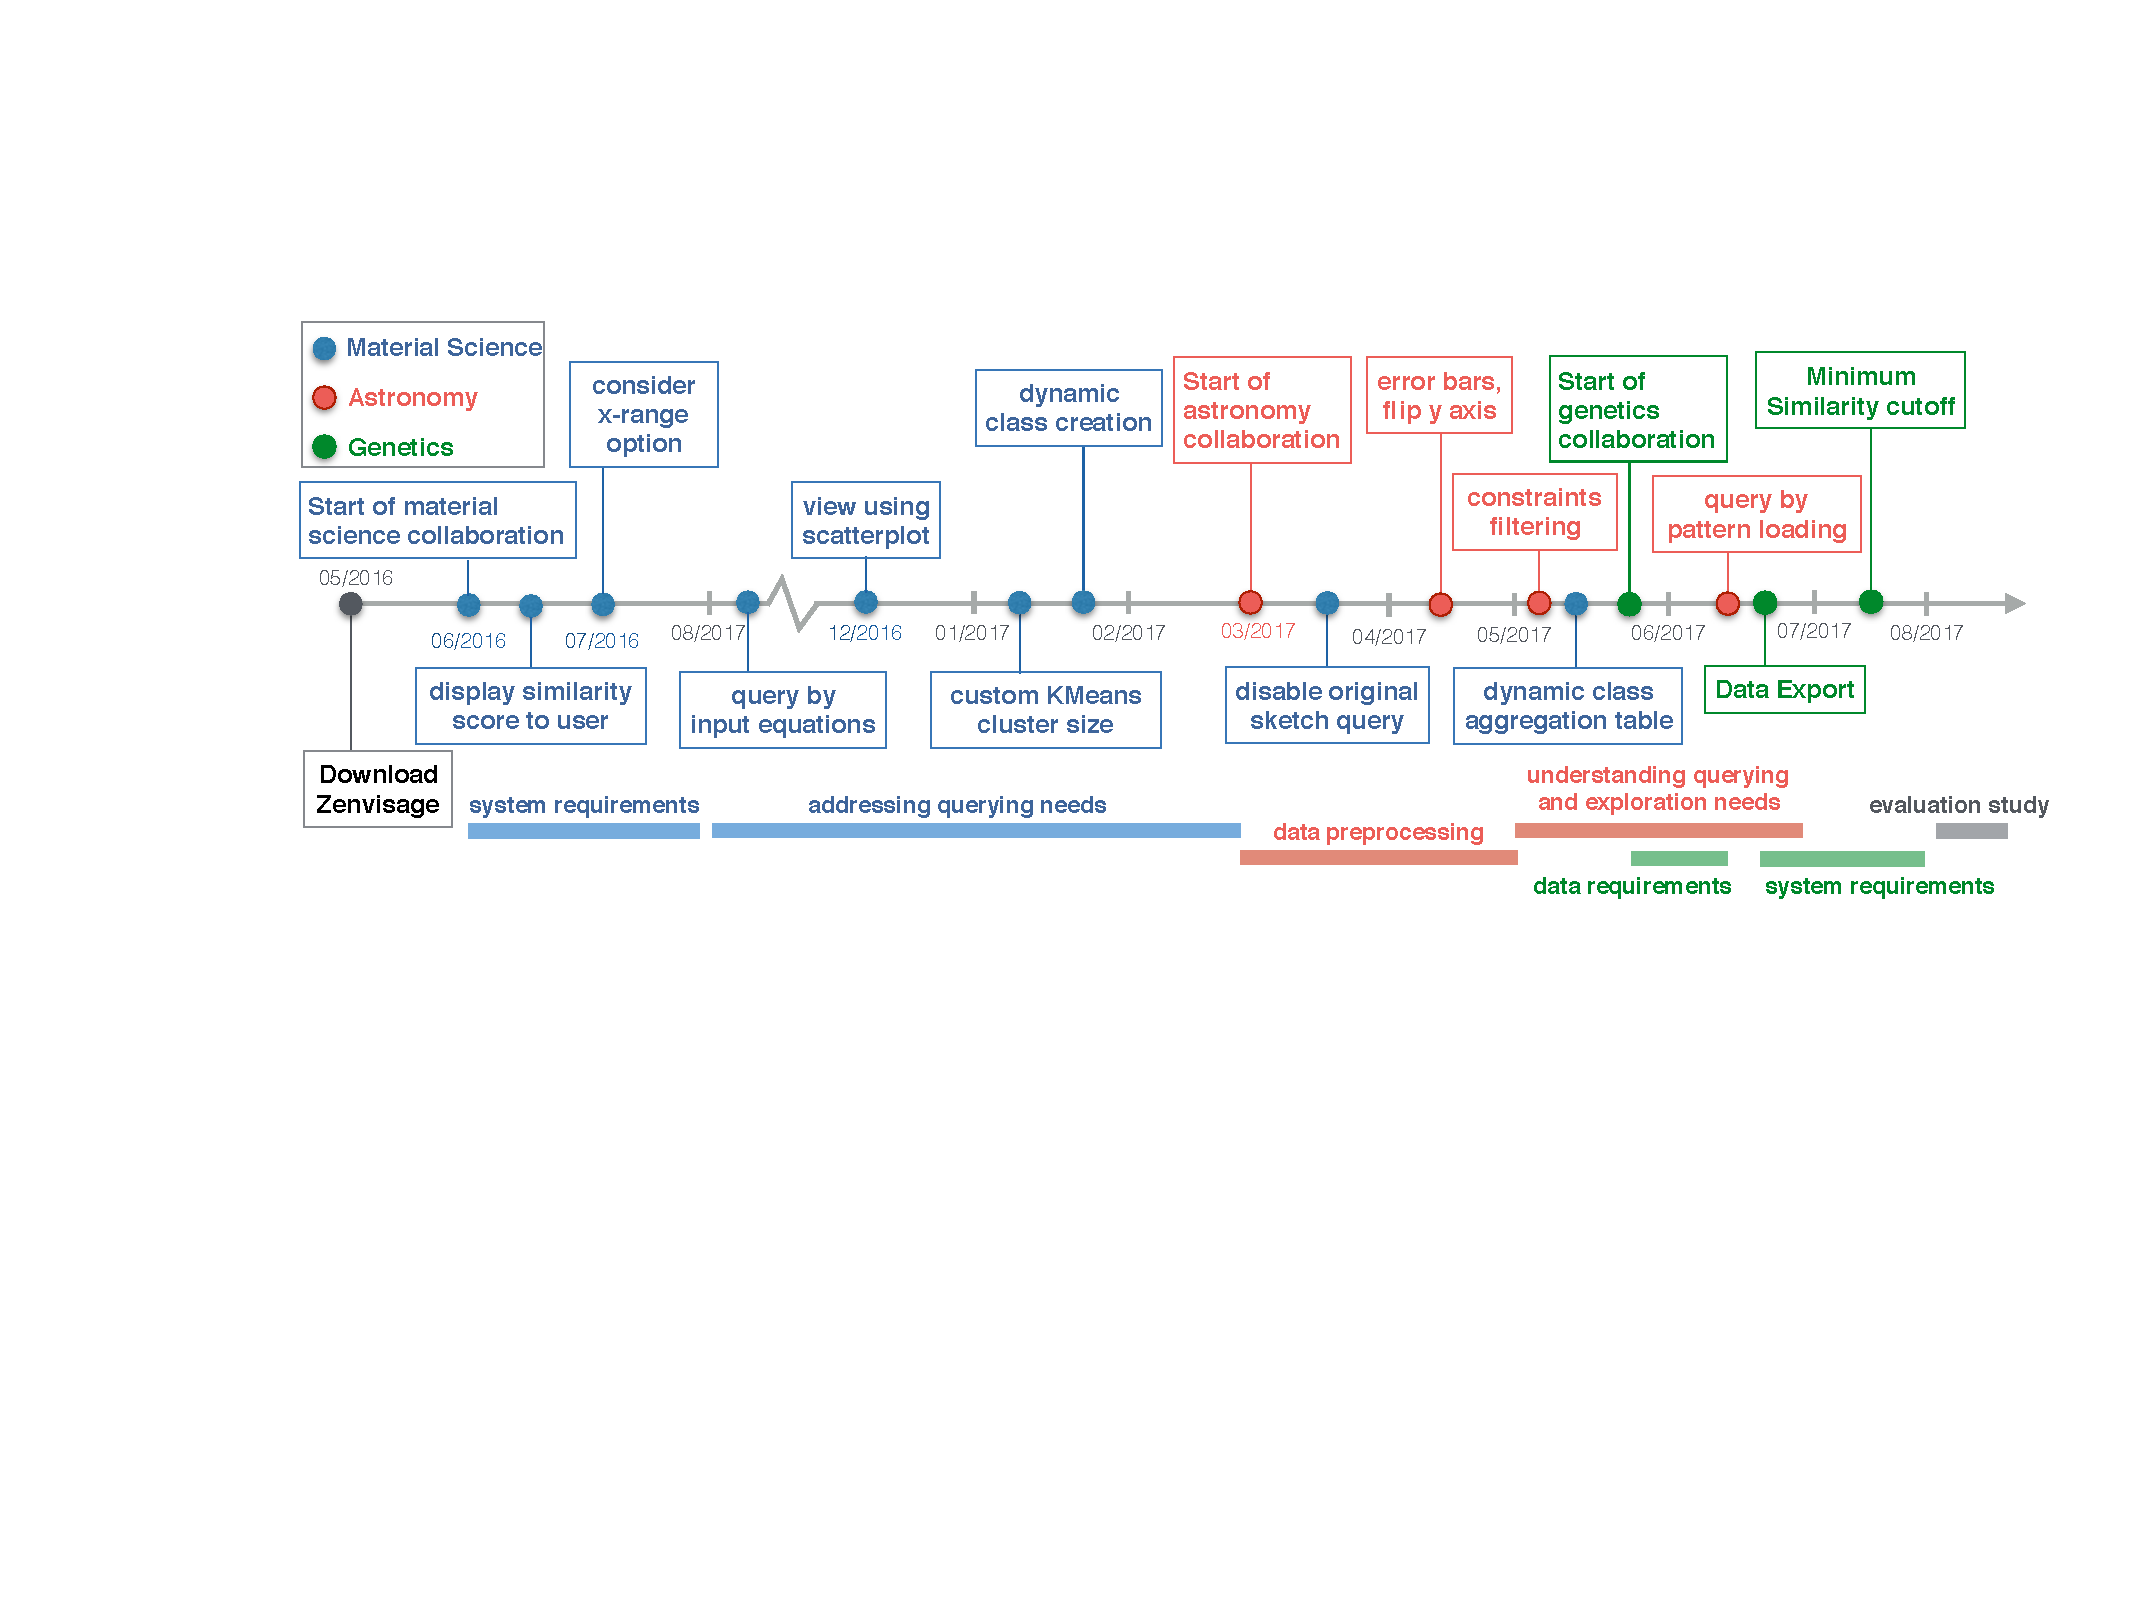
\includegraphics[width=6in]{figures/timeline_anon.pdf}
	\vspace{-6pt}\caption{Timeline for progress in participatory design studies.}
	\label{timeline}
	\vspace{-10pt}
\end{figure*}
\par Via cognitive walkthroughs and interviews, we first identified challenges in existing data analysis workflows in these domains
that could be potentially addressed by a VQS. Building on top of an existing, open-source VQS, \zv~\cite{Siddiqui2017,Siddiqui2017VLDB}, we collaborated closely with our participants to gather feedback and iterate on VQS feature designs,
over the course of a year, culminating in a new enhanced VQS, \zvpp. We organized these features into a taxonomy of VQS functionalities, involving three sensemaking processes inspired by Pirolli and Card's notional model of analyst sensemaking~\cite{Pirolli}. The sensemaking processes include top-down pattern specification (translating a pattern ``in-the-head'' into the form of a visual query), bottom-up data-driven inquiries (querying or recommending based on data), and context-creation (navigating across different collections of visualizations). We find that prior VQSs have focused largely on top-down processes, while largely ignoring the other two processes that are crucial for the needs in all three domains.
\par To study how various VQS features
are used in practice,
we conducted a final evaluation study with nine participants
using our final VQS prototype, \zvpp,
to address their research questions
on their own datasets.
In a 1.5-hour user study, participants were able to
gain novel scientific insights,
such as identifying a star with a transient pattern
that was known to harbor a Jupiter-sized planet
and finding characteristic gene expression profiles confirming the results of a related publication.\techreport{, and discovering that the dip in an astronomical light curve is caused by saturated imaging equipment overlooked by the existing error-detection pipeline.} \techreport{Participants also gain additional insights about their datasets, including debugging mislabeled features and uncovering erroneous data preprocessing procedure applied to a collaborator's dataset.}
%that goes from a pattern in-the-head to a desired visualization

\par By analyzing the evaluation study results, we discovered that sketching a pattern for querying is often ineffective. This is due to the fact that sketching makes the problematic assumptions that users know the pattern that they want to sketch and are able to sketch it precisely. Instead, participants typically opted for other means of pattern specification---one common mechanism was to drag-and-drop a recommended pattern onto the canvas, and then modify it (e.g., by smoothing it out). However, most VQSs do not support these other mechanisms (as we argued earlier, they typically focus only on top-down sensemaking processes, without covering bottom-up and context creation), partially explaining why such systems have not been widely adopted in practice.
\par Further analysis of how participants
transition between different sensemaking processes
during analysis---including the construction of a Markov Model---illustrated
how participants adopt a diverse set of workflows tailored
to their domains. We find that participants often construct analysis workflows focused around a primary sensemaking process, while iteratively interleaving their analysis with the two other processes. This finding points to how all three sensemaking processes, along with seamless transitions between them, are essential for enabling users to effectively use VQSs for data exploration.%For example, participants often center on a main sensemaking process, while interleaving variations with other two processes as they iterate on an analytic task.
\par To the best of our knowledge, our study is the \emph{first to holistically examine how VQSs can be designed to fit the needs of real-world
analysts and how they are actually used in practice}. Our contributions include:
\begin{denselist}
\item a characterization of the problems addressable by VQSs through design studies with three different domains,
\item the construction of a taxonomy of functionalities within VQSs, as well as an articulation of the problem space that is amenable to VQSs, both grounded in participatory design findings,
\item \change{an integrative} VQS, \zvpp, capable of facilitating rapid hypothesis generation and insight discovery,
\item study findings on how VQSs are used in practice, leading to the development of a novel sensemaking model for VQSs. %including the ineffectiveness of
%evaluation
% sketching and the ---- workflow
\end{denselist}
Our work not only opens up a new space of opportunities beyond the narrow use cases considered by prior studies, but also advocates common design guidelines and end-user considerations for building next-generation VQSs.
 %From these experiences, we  advocate visualization researchers and tool designers to ---- future VQS opportunities  Understanding the design space and opportunities for VQS
% Our three main research questions are as follows:

%and not as commonly ---- due to the --- challenges ----. that ----- characteristic workflows ---- iterative sensemaking loop.
%Our collaborative design experience culminated in a full-fledged VQS, \zvpp, described in Section~\ref{sec:pd_findings}.
% \noindent \emph{RQ1: What are the challenges in existing scientific data analysis workflows that could be potentially addressed by a VQS?}
% \par Via cognitive walkthroughs and interviews,
% we gained an understanding of the data analysis
% workflows presently employed by the scientists, their needs,
% and the challenges they face.
% We identified opportunities where a VQS could
% help accelerate their analysis, by helping them
% discover insights, gain intuition, or provoke directions
% for exploration. Finally, we determined the types of
% research questions and dataset properties that would
% be most suitable for exploration on VQSs.
%By learning about the needs and challenges that scientists face when working with their datasets through interviews and cognitive walkthroughs, we learned about the types of queries that they would like to pose on VQSs and distilled a set of design specifications that can better enable VQSs to help them discover insights, gain intuition about their datasets or provoke further directions for exploration. We also identify the types of research questions and dataset properties would be suitable for data exploration on VQSs.
% \begin{figure*}[ht!]
% \centering
% \vspace{-15pt}
% 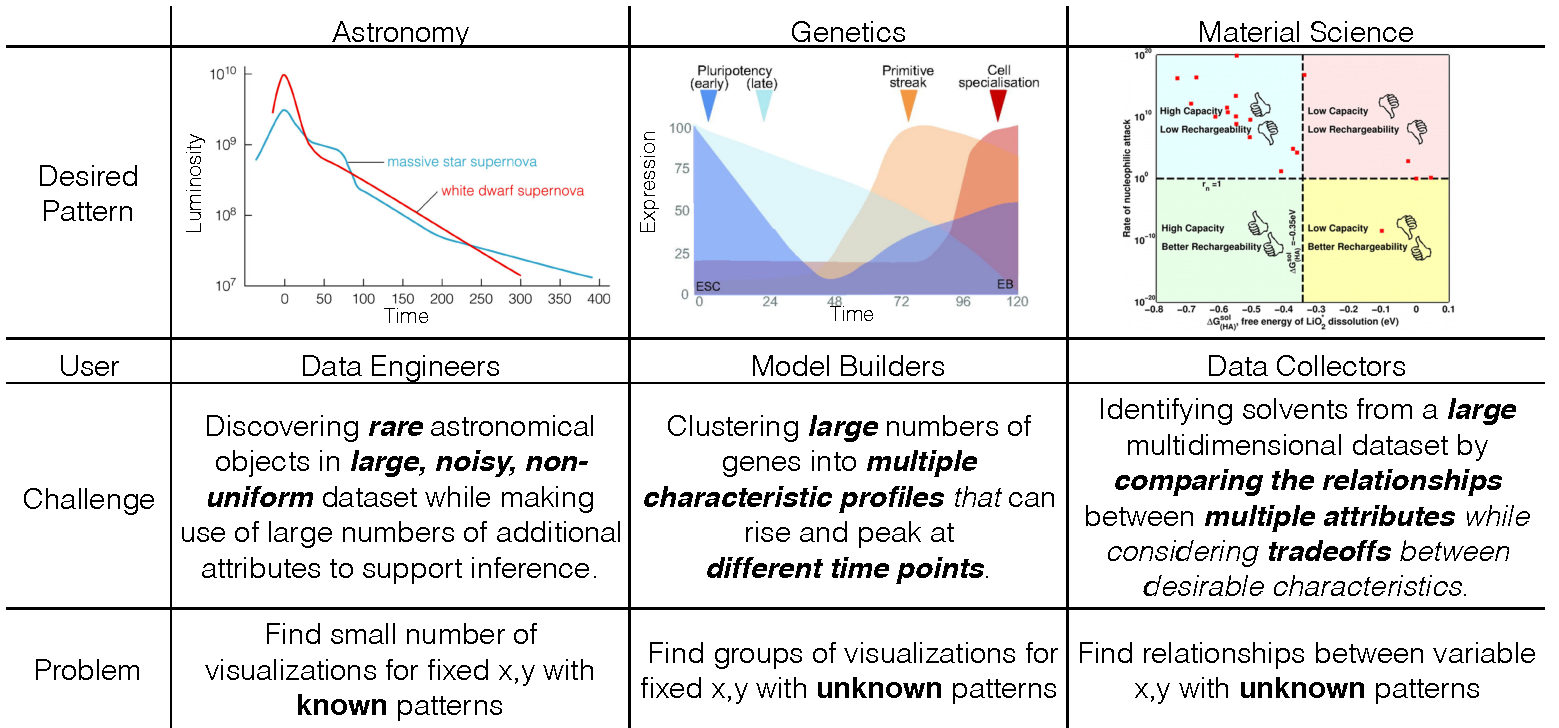
\includegraphics[width=0.8\linewidth]{figures/sci_challenge_tbl.pdf}
% \vspace{-6pt}\caption{Descriptions of the three scientific use cases discussed in this paper.}
% \label{example}
% \vspace{-10pt}
% \end{figure*}

% \noindent \emph{RQ2: What types of interface capabilities are necessary to develop VQSs into a useful component of data analysis?}
% \par Via participatory design, we distilled
% \tvcg{Based on our early interactions with scientists,
% we started to build a VQS~\cite{Siddiqui2017VLDB,Siddiqui2017} that, similar to existing VQSs~\cite{wattenberg2001sketching}, allowed them to search for desired trends via drawing on a canvas. This early system served as a functional prototype for us to engage with scientists further in the participatory design process, understand how they envision themselves using a VQS, and gather feedback on feature designs that could make the VQS more useful. The features we developed address challenges shared across the three scientific domains, ranging from additional querying modalities, to features that support a more integrated workflow, to improving the interpretability of the system output, \tvcg{most of them missing in} prior VQSs in the literature. Our collaborative design experience culminated in a full-fledged VQS, \zv, capable of facilitating rapid hypothesis generation and insight discovery.}

% \noindent \emph{RQ3: How do VQSs accelerate scientific insights?} and \emph{RQ4: How can VQSs fit within the context of existing data analysis workflows?}
% \\ To evaluate our final system \zv, we conducted a user study with nine scientists (including those who had participated in the design process), all of whom had a vested interest in using a VQS to address their research questions on their datasets. In a 1.5-hour user study, our scientist participants were able to gain novel scientific insights, such as \emph{\tvcg{identifying a star with a transient pattern that was known to harbor a Jupiter-sized planet,} finding characteristic gene expression profiles that confirmed the results of a related publication, and learning that the dip in an astronomical light curve is caused by saturated imaging equipment overlooked by the existing error-detection pipeline}.  Participants also gained additional insights about their datasets, including debugging \tvcg{mislabelled features and uncovering the erroneous data preprocessing procedure applied to a collaborator's dataset.}
% that the way data is aggregated across multiple experiments is erroneous on a collaborator's dataset.
% We learned how VQSs could be contextualized within scientific data analysis workflows and discovered that VQSs can be used beyond the exploratory phase of analysis, for data verification, debugging preliminary datasets, and performing sanity-checks on downstream models.

% \begin{figure}[h!]
%     \centering
%     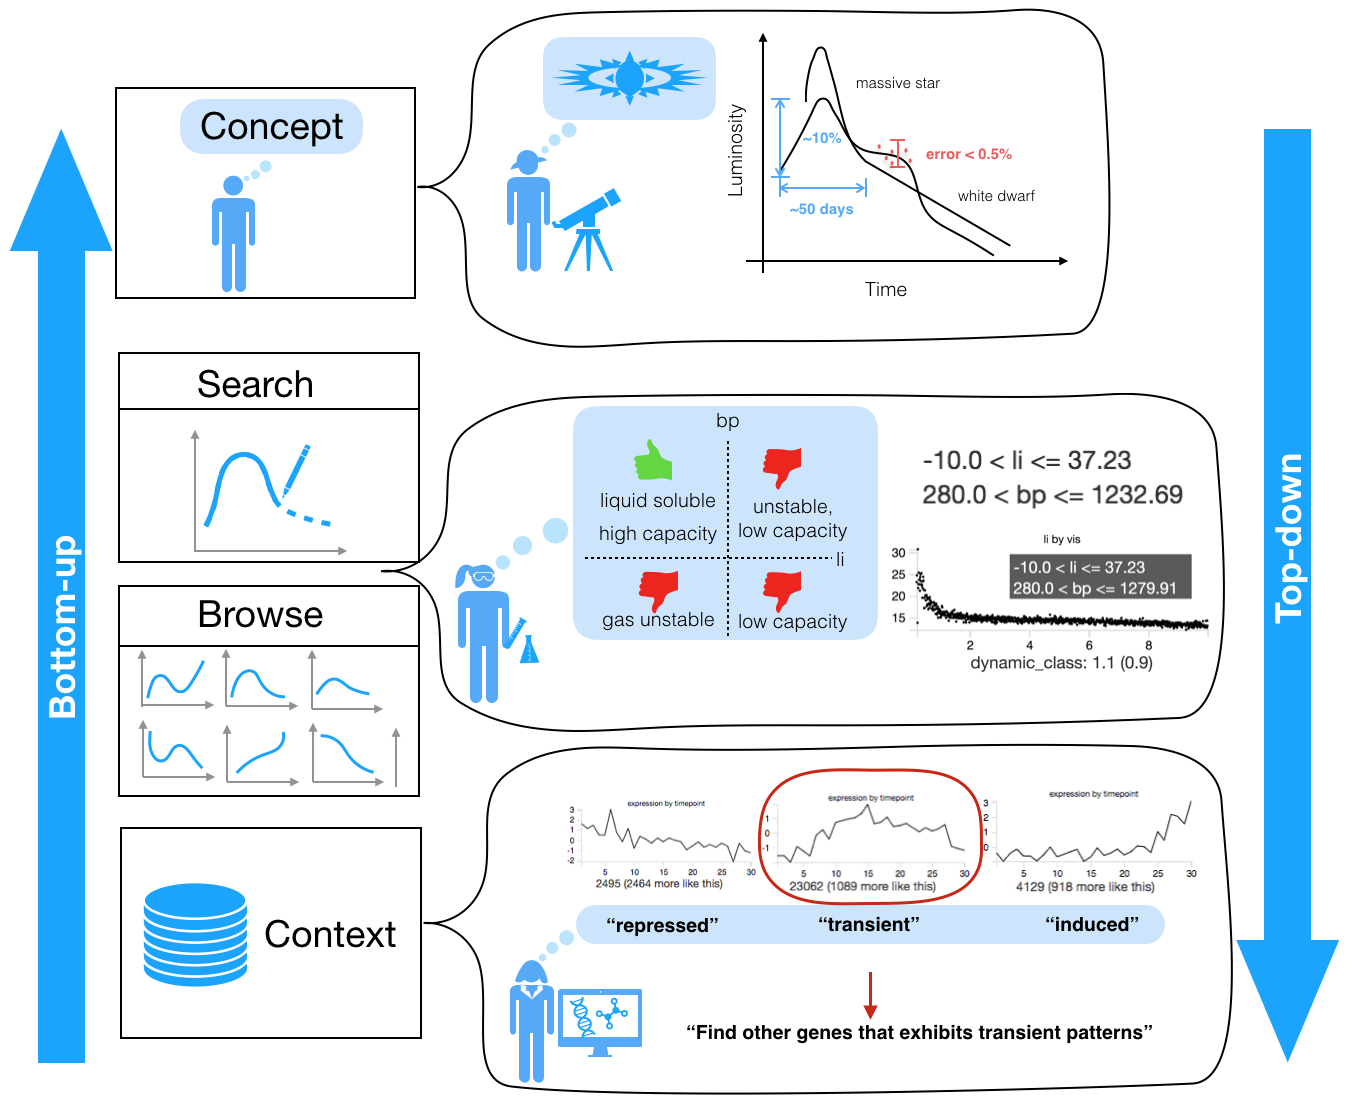
\includegraphics[width=\linewidth]{figures/search-browse-model.png}
%     \vspace{-6pt}\caption{Search Browse Model}
%     \label{fig:sbmodel}
%     \vspace{-5pt}
% \end{figure}

%!TEX root = main.tex
\section{Methods\label{sec:methods}}
\subsection{Background and Motivation}
\par Visual query systems enable users to directly search for visualizations matching certain patterns through an intuitive specification interface. Early work in this space focused on interfaces to search for time series of interest, including TimeSearcher~\cite{Hochheiser2001,Hochheiser2004}, where the query is composed of one or more rectangular value-range selections, and QuerySketch~\cite{wattenberg2001sketching} and Google Correlate~\cite{mohebbi2011google}, where the query is sketched as a pattern. Subsequent work recognized the ambiguity of sketches and improved the expressiveness of sketched queries through finer specification interfaces and pattern-matching algorithms~\cite{ryall2005querylines,Holz2009}, as well as performed crowdsourced perceptual studies to understand how humans rank similarity in patterns subjectively~\cite{Eichmann2015,correll2016semantics,Mannino2018}. Table~\ref{table:relatedwork} summarizes the list of features offered by these existing systems.
% , including the use of soft constraints~\cite{ryall2005querylines} and implicit relaxed selection techniques~\cite{Holz2009}. 
% In addition to this ongoing work, recent work have also performed crowdsourced perceptual studies to understand how humans rank similarity in patterns subjectively~\cite{Eichmann2015,correll2016semantics,Mannino2018}. 
\begin{table*}[ht!]
    \begin{tabular}{l
    >{\columncolor[HTML]{67FD9A}}l
    >{\columncolor[HTML]{67FD9A}}l
    >{\columncolor[HTML]{67FD9A}}l
    >{\columncolor[HTML]{67FD9A}}l
    >{\columncolor[HTML]{FD6864}}l
    >{\columncolor[HTML]{FD6864}}l
    >{\columncolor[HTML]{FD6864}}l
    >{\columncolor[HTML]{FD6864}}l
    >{\columncolor[HTML]{FD6864}}l }
                                                      & \multicolumn{1}{c}{\cellcolor[HTML]{DAE8FC}{\color[HTML]{000000}  \thead{Freehand \\ Sketching}}} & \multicolumn{1}{c}{\cellcolor[HTML]{DAE8FC}{\color[HTML]{000000}  \thead{Shape \\ Approx.}}} & \multicolumn{1}{c}{\cellcolor[HTML]{DAE8FC}{\color[HTML]{000000}  \thead{Range \\ Selection}}} & \multicolumn{1}{c}{\cellcolor[HTML]{DAE8FC}{\color[HTML]{000000} \thead{Flexible\\ Matching}}} & \multicolumn{1}{c}{\cellcolor[HTML]{FFCE93}{\color[HTML]{000000} \thead{Filter \\ Selection}}} & \multicolumn{1}{c}{\cellcolor[HTML]{FFCE93}{\color[HTML]{000000} \thead{Group\\ Comparison}}} & \multicolumn{1}{c}{\cellcolor[HTML]{FFFFC7}\thead{Concept\\ Querying}} & \multicolumn{1}{c}{\cellcolor[HTML]{FFFFC7}\thead{Result\\ Querying}} & \multicolumn{1}{c}{\cellcolor[HTML]{FFFFC7}\thead{Recommend \\ Result}} \\
    Timesearcher \cite{Hochheiser2001,Hochheiser2004} & \cellcolor[HTML]{FD6864}{\color[HTML]{000000} }                                        &                                                                                                                               &                                                                                                                                & \cellcolor[HTML]{FD6864}{\color[HTML]{FE0000} }                                       & {\color[HTML]{FE0000} }                                                              & {\color[HTML]{FE0000} }                                                              & {\color[HTML]{FE0000} }                                       & \cellcolor[HTML]{67FD9A}                                     & {\color[HTML]{FE0000} }                                    \\
    QuerySketch \cite{wattenberg2001sketching}        &                                                                                        & \cellcolor[HTML]{FD6864}                                                                                                      &                                                                                                                                & \cellcolor[HTML]{FD6864}                                                              &                                                                                      &                                                                                      &                                                               &                                                              &                                                            \\
    QueryLines \cite{ryall2005querylines}             &                                                                                        &                                                                                                                               &                                                                                                                                &                                                                                       &                                                                                      &                                                                                      &                                                               &                                                              &                                                            \\
    SoftSelect \cite{Holz2009}                        &                                                                                        &                                                                                                                               & \cellcolor[HTML]{FD6864}                                                                                                       &                                                                                       &                                                                                      &                                                                                      &                                                               &                                                              &                                                            \\
    Google Correlate \cite{mohebbi2011google}         & \cellcolor[HTML]{67FD9A}                                                               & \cellcolor[HTML]{FD6864}                                                                                                      & \cellcolor[HTML]{FD6864}                                                                                                       &                                                                                       &                                                                                      &                                                                                      & \cellcolor[HTML]{67FD9A}                                      &                                                              & \cellcolor[HTML]{67FD9A}                                   \\
    TimeSketch \cite{Eichmann2015}                    &                                                                                        & \cellcolor[HTML]{FD6864}                                                                                                      & \cellcolor[HTML]{FD6864}                                                                                                       & \cellcolor[HTML]{FD6864}                                                              &                                                                                      &                                                                                      &                                                               &                                                              &                                                            \\
    SketchQuery \cite{correll2016semantics}           &                                                                                        &                                                                                                                               & \cellcolor[HTML]{FD6864}                                                                                                       &                                                                                       &                                                                                      &                                                                                      &                                                               & \cellcolor[HTML]{67FD9A}                                     &                                                            \\
    Qetch \cite{Mannino2018}                          &                                                                                        &                                                                                                                               &                                                                                                                                &                                                                                       &                                                                                      &                                                                                      &                                                               &                                                              & \cellcolor[HTML]{67FD9A}                                   \\
    Zenvisage                                         &                                                                                        &                                                                                                                               &                                                                                                                                &                                                                                       & \cellcolor[HTML]{67FD9A}                                                             & \cellcolor[HTML]{67FD9A}                                                             & \cellcolor[HTML]{67FD9A}                                      & \cellcolor[HTML]{67FD9A}                                     & \cellcolor[HTML]{67FD9A}
    \end{tabular}
    \caption{Table summarizing the key components of VQSs (columns) covered by past systems (row). Green indicates that feature exist in the system; red indicate feature not covered. Column header colors blue, orange, yellow covers processes: top-down querying, search with context, and bottom-up querying respectively, described more in Section~\ref{sec:guidelines}. }
\end{table*}

\par While these systems have been shown to be effective for visual querying in controlled lab studies, they have not been evaluated in-situ on real-world use cases. In this work, we adopted a mixed methods research methodology that draws inspiration from ethnographic methods, iterative and participatory design, and controlled studies~\cite{Plaisant2004,lam2012empirical,miller_salkind_miller_2002,shneiderman2006strategies,Muller1993} to more thoroughly understand the design space of VQSs and how various components of VQSs are used in practice. Participatory design has been successfully used in the development of interactive visualization systems in the past~\cite{Aragon2008,Chuang2012}. Sedlmair et al. \cite{Sedlmair2012} advocate that design study methodology is suitable for use cases in which the data is available for prototyping, but the task is only partially known and the information is partially in the user's head. %to understand how VQSs can be used in scientific data analysis. %In that regard, our scientific use cases with VQS is well-suited for a design study methodology, as we learn about the scientist's data and analysis requirements and design interactions that helps users translate their ``in-the-head'' specifications into actionable visual queries.
\subsection{Participatory Design}
\par  Working with researchers from three different scientific research groups, we identified the needs and challenges of scientific data analysis and potential opportunities for VQSs, via interviews and cognitive walkthroughs. We recruited participants by reaching out to research groups via email and word of mouth, who have experienced challenges in dealing with large amounts of data. We initially spoke to analysts from 12 different potential application areas and narrowed down to three use cases in astronomy, genetics, and material science for our participatory design study, based on their suitability for VQS as well as diversity in use cases. Six scientists from three research groups participated in the design of \zv. On average, participants had more than 8 years of research experience working in their respective fields. %\techreport{We list the participants in Table~\ref{participants}, and will refer to them by their anonymized ID as listed in the table throughout the paper.}
\par Given our early conversations with participants, we built a basic VQS to serve as the functional prototype in the design study. This early VQS prototype allowed users to sketch a pattern or drag-and-drop an existing visualization as a query, then the system would return visualizations that had the closest Euclidean distance from the queried pattern. The details of the system is described in \cite{Siddiqui2017,Siddiqui2017VLDB}, which focused on the system and scalability aspects of the VQSs.
	% \begin{figure}[ht!]
	% \centering
	% 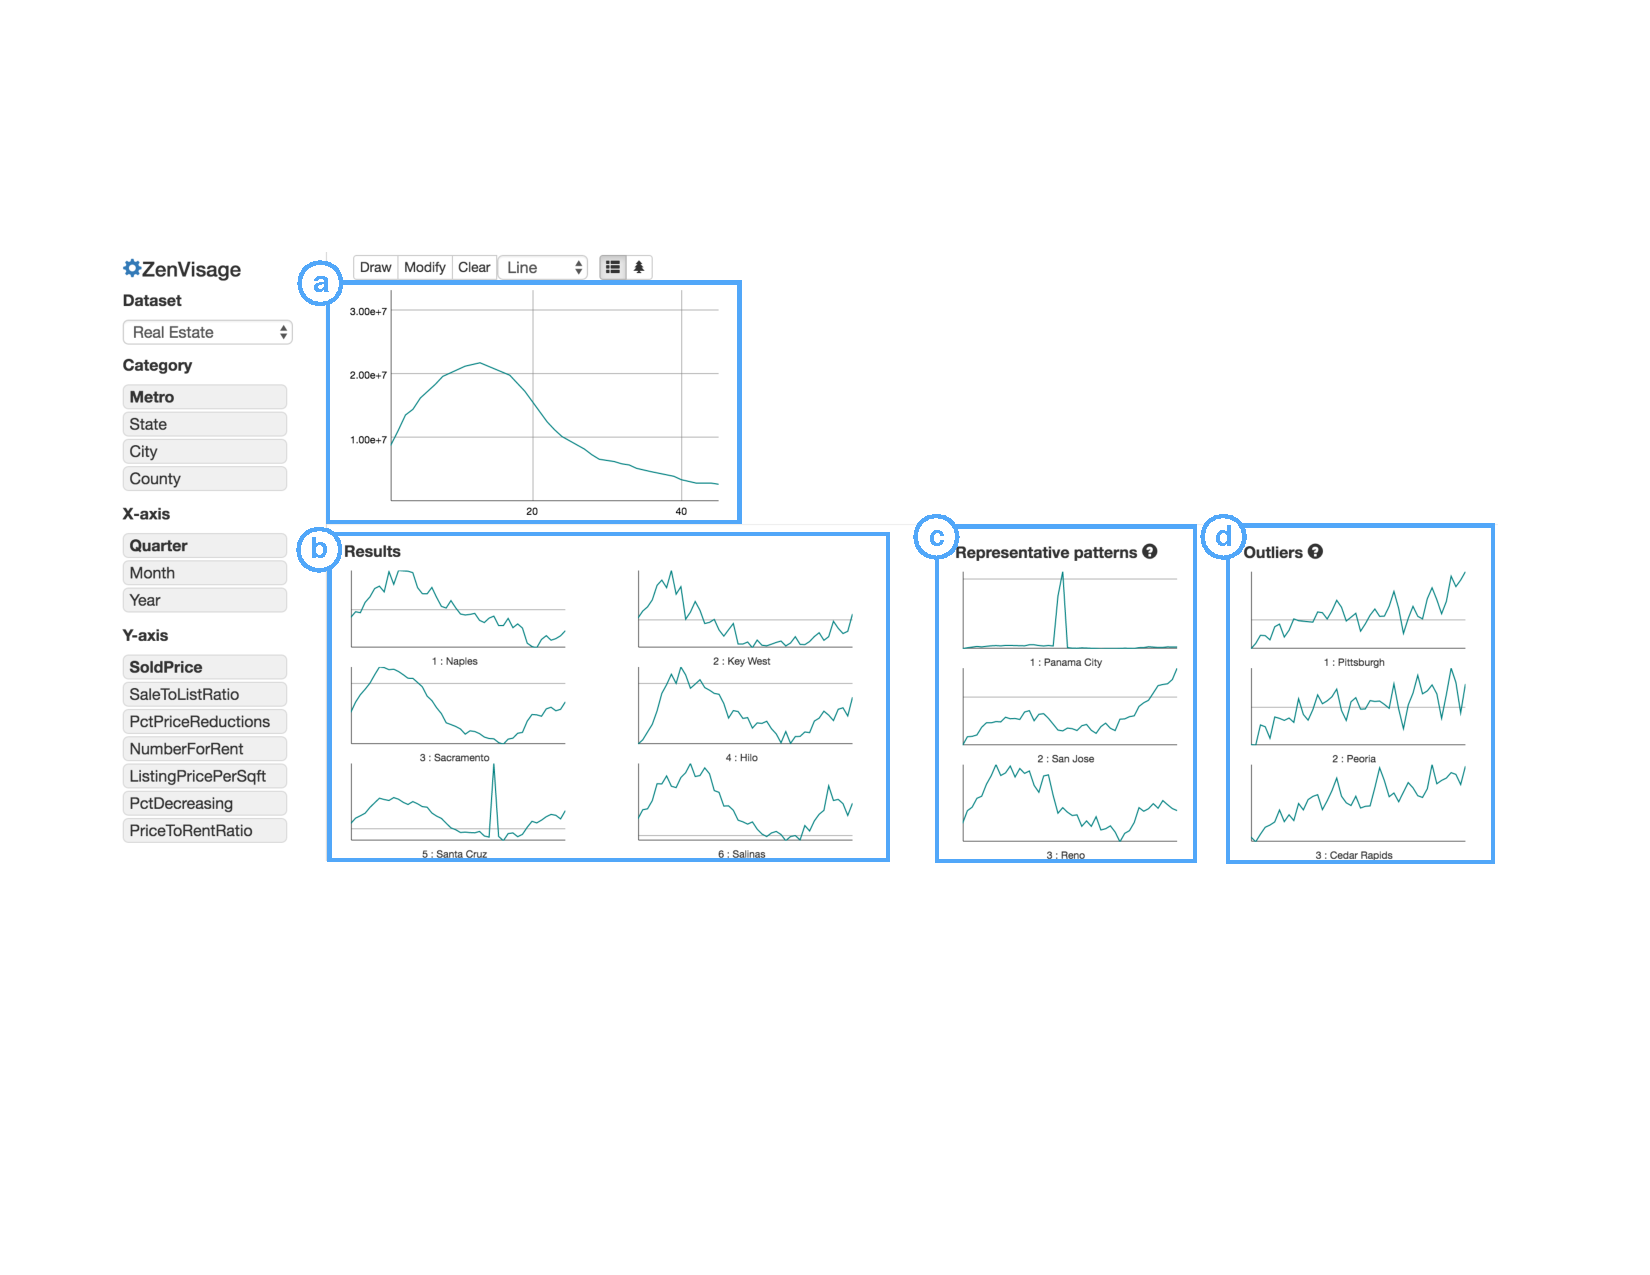
\includegraphics[width=\linewidth]{figures/oldZV_nozql.pdf}
	% \caption{The \zv prototype allowed users to sketch a pattern in (a), which would then return (b) results that had the closest Euclidean distance from the sketched pattern. The system also displays (c) representative patterns obtained through K-Means clustering and (d) outlier patterns to help the users gain an overview of the dataset.}
	% \label{oldZV}
	% \end{figure}
\par The use of functional prototypes is common and effective in participatory design to provide a starting point for the participants, as studied by Ciolfi et al.\cite{Ciolfi2016}. %For example, Ciolfi et al.\cite{Ciolfi2016} studied two different alternatives to co-design (starting with open brief versus functional prototype) in the development of museum guidance systems and found that while both approaches were equally fruitful, functional prototypes can make addressing a specific challenge more immediate and focused. 
Our motivation for providing a functional prototype at the beginning of the participatory design sessions is to showcase capabilities of VQSs. Especially since VQSs are not common in the existing workflows of these scientists, participants may not be able to imagine their use cases without a starting point.
\par During the participatory design process, we collaborated with each of the teams closely with an average of two meetings per month, where we learned about their datasets, objectives, and how VQSs could help address their research questions. A summary timeline of our engagement with the participants and the features inspired by their use cases can be found in Figure \ref{timeline}. Participants provided datasets they were exploring from their domain, whereby they had a vested interest in using a VQS to address their own research questions. Through this process, we identified and incorporated more than 20 desired features into our VQS prototype, \zv, over the period of a year.
\begin{figure*}[!ht]
	\centering
	\captionsetup{justification=centering,margin=2cm}
	\vspace{-10pt}
	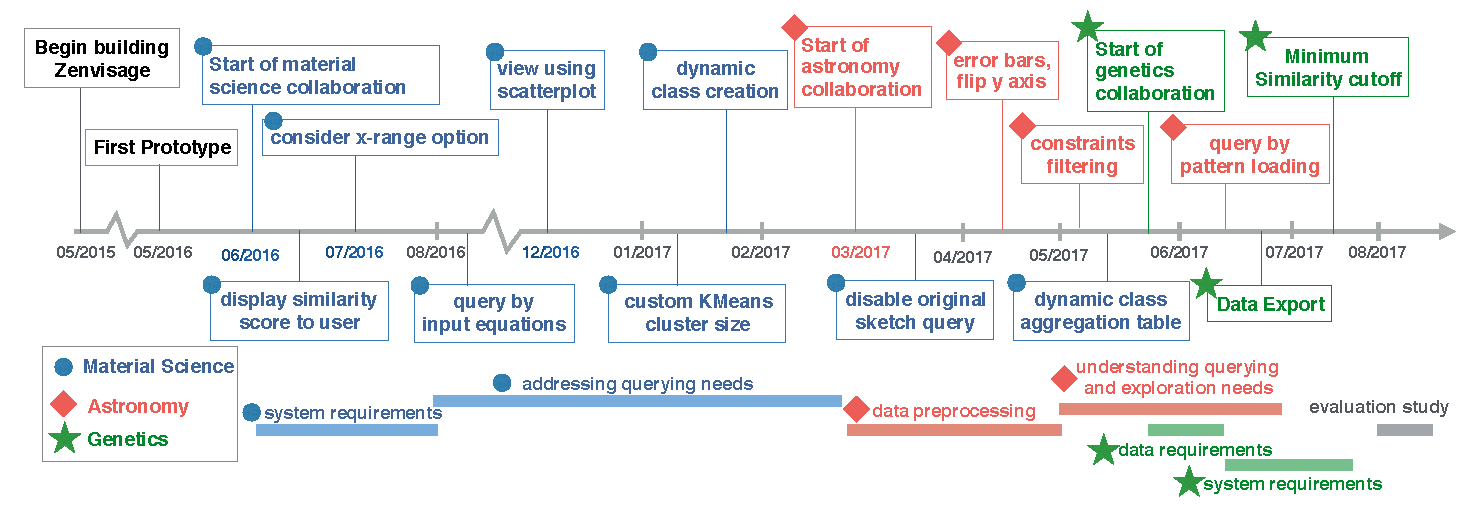
\includegraphics[width=6in]{figures/timeline_new.pdf}
	\vspace{-6pt}\caption{Participatory design timeline for the scientific use cases.}
	\label{timeline}
	\vspace{-10pt}
\end{figure*}
\subsection{Evaluation Study}
\par Visualization systems are often evaluated using controlled studies that measure the user's performance against an existing visualization baseline~\cite{Plaisant2004}. Techniques such as artificially inserting ``insights'' or setting predefined tasks for example datasets work well for objective tasks, such as debugging data errors~\cite{kandel2011wrangler,Patel2010}, but these contrived methods are unsuitable for trying to learn about the types of real-world queries users may want to pose on VQSs. %Due to the unrealistic nature of controlled studies, many have proposed using a more multi-faceted, ethnographic approach to understand how analysts perform visual data analysis and reasoning~\cite{Plaisant2004,lam2012empirical,shneiderman2006strategies,munzner2009nested,Sedlmair2012}. 
In order to make the evaluation more realistic, at the end of our participatory design study, we opted for a qualitative evaluation where we invited participants to bring datasets that they have vested interests in to address unanswered research questions, in order to study how analysts interact with different VQS components in practice.
\par The evaluation study participants included the six scientists from participatory design, along with three additional ``blank-slate'' participants who had never encountered \zv before. While participatory design subjects actively provided feedback on \zv with their data, they only saw us demonstrating their requested features and explaining the system to them, rather than actively using the system on their own. So the evaluation study was the first time that all participants used \zv to explore their datasets.
\par Participants for the evaluation study were recruited from each of the three aforementioned research groups, as well as domain-specific mailing lists. Prior to the study, we asked the potential participants to fill out a pre-study survey to determine their eligibility. Eligibility criteria included: being an active researcher in the subject area with more than one year of research experience, and having worked on a research project involving data of the same nature as that used in the participatory design. Four of the evaluation studies were conducted remotely. Participants had the option of exploring their own dataset or an existing dataset that they provided to us during the participatory design process. All three blank-slate participants opted to explore their own datasets. %After loading their dataset, we emailed them a screenshot of a visualization from our tool to verify that we configured the system to meet their needs.
\par At the start, participants were provided with an interactive walk-through explaining the system details and given approximately ten minutes to experience a guided exploration of our VQS with a preloaded real-estate example dataset from Zillow \cite{zillow}.\techreport{This dataset contained housing data for various cities, metropolitan areas, and states in the U.S. from 2004-15.} After familiarizing themselves with the tool, we loaded the participant's dataset and encouraged them to talk-aloud or use external tools as needed during the data exploration phase.% and suggested an appropriate choice of axis to begin the exploration. 
%\par During the exploration phase, participants were informed that they could use other tools as needed. 
If the participant was out of ideas\ccut{ for three minutes}, we suggested one of the ten main functionalities in \zv \techreport{\footnote{query by sketching, drag-and-drop, pattern loading, input equations, representative and outliers, narrow/ignore x-range options, filtering, data smoothing, creating dynamic classes,  data export}}that they had not yet used. If any of these operations were not applicable to their specific dataset, they were allowed to skip the operation after having considered how it may or may not be applicable to their workflow. The user study ended after they covered all ten main functionalities. On average, the main exploration phase lasted for 63 minutes. After the study, we asked them open-ended questions about their experience.
%!TEX root = main.tex
\section{Participants and Datasets\label{sec:participantdatasets}}
At the start of our design study, \change{we conducted contextual inquiry to learn about our participants'} existing data analysis workflows. Next, we describe our study participants\change{, their scientific goals, } and their preferred analysis workflows. \change{Note that while we have collaborated with each application domain in depth, due to the space limitation of the paper, we summarize the key findings in each domain to highlight their commonalities and differences, in order to provide a backdrop for generalized VQSs findings described later in the paper.}
%use cases to highlight behaviors that participants have adopted for conducting certain analysis tasks.
\par\noindent\stitle{Astronomy:} The Dark Energy Survey is a multi-institution project that surveys 300 million galaxies over 525 nights to study dark energy~\cite{Drlica-Wagner2017}. The telescope used to survey these galaxies also focuses on smaller patches of the sky on a weekly interval to discover astronomical transients (objects whose brightness changes dramatically as a function of time), such as supernovae or quasars. Their dataset consists of a large collection of \change{\emph{light curves}: brightness observations over time, one associated with each astronomical object, plotted as time series. Over} five months, we worked closely with A1, an astronomer on the project's data management team working at a supercomputing facility. Their scientific goal is to identify potential astronomical transients in order to study their properties. \techreport{These insights can help further constrain physical models regarding the formation of these objects.}
\npar To identify transients, astronomers programmatically generate visualizations of candidate objects with \texttt{matplotlib} and visually examine each light curve. While an experienced astronomer who has examined many transient light curves can often distinguish an interesting transient object from noise by sight, manual searching for transients is time-consuming and error prone, since the large majority of the objects are false positives. A1 was interested in VQSs as he recognized how specific pattern queries could help astronomers directly search for these rare transients.
\techreport{\par If an object of interest or region is identified through the visual analysis, then the astronomer may be interested in inspecting the image of the region for cross-checking that the significant change in brightness of the object is not due to an imaging artifact. This could be done using a custom built web-interface that facilitates the access of cutout images for a queried region of the sky.}
\par\noindent\stitle{Genetics:} Gene expression is a common measurement in genetics obtained via microarray experiments~\cite{Peng2016}. \techreport{In these experiments, a grid containing thousands of DNA fragments are exposed to stimuli and measurements for the level at which a gene is expressed are recorded as a function of time.} We worked with a graduate student (G1) and professor (G3) at a research university who were using gene expression data to understand how genes are related to phenotypes expressed during early development\techreport{\cite{Peng2016,Gloss2017}}. Their data consisted of a collection of gene expression profiles over time for mouse stem cells, aggregated over multiple experiments.\techreport{, downloaded from an online database\footnote{\url{ncbi.nlm.nih.gov/geo/}}.} %They were interested in using \zv to cluster gene expression data before conducting analysis with a downstream machine learning workflow.
\npar Their typical workflow is as follows: G1 first loads the preprocessed gene expression data into a custom desktop application for visualizing and clustering it\techreport{\footnote{\url{www.cs.cmu.edu/~jernst/stem/}}}. After setting several system parameters and executing the clustering algorithm, the overlaid time series for each cluster is displayed on the interface. G1 visually inspects that the patterns in each cluster looks ``clean'' and checks that the number of outlier genes (i.e., those that do not fall into any of the clusters) is low.  If the number of outliers is high or the clustered visualizations look ``unclean'', she reruns the analysis by increasing the number of clusters. Once the visualized clusters look ``good enough'', G1 exports the clusters to her downstream regression tasks.
\npar Prior to the study, G1 and G3 spent over a month attempting to determine the best number of clusters based on a series of static visualizations and statistics computed after clustering. While regenerating their results took no more than 15 minutes every time they made a change, the multi-step, segmented workflow meant that all changes had to be done offline.\techreport{, so that valuable meeting time was not wasted trying to regenerate results.} \change{They were interested in VQSs as interactively querying time series with clustering results could dramatically speed up their collaborative analysis process.}
%The team were interested in VQSs as they saw how interactively querying time series with clustering results could dramatically speed up their collaborative analysis process.
%that can improve battery performance and stability
\par\noindent\stitle{Material Science:} We collaborated with material scientists at a research university who are working to identify solvents for energy efficient and safe batteries. These scientists work on a large simulation dataset containing chemical properties for more than 280,000 solvents~\cite{Khetan2018}. Each row of their dataset represents a unique solvent with 25 different chemical attributes. We worked closely with a a postdoctoral researcher (M1), professor (M2), and graduate student (M3) for over a year to design a sensible way of exploring their data. They wanted to use VQSs to identify solvents that not only have similar properties to known solvents\change{,} but are also more favorable (e.g., cheaper or safer to manufacture). To search for these desired solvents, they need to understand how changes in certain chemical attributes affect other properties under specific conditions.
\npar M1 typically starts his data exploration process by iteratively applying filters to a list of potential battery solvents using SQL queries. \change{Once the remaining solvent list is sufficiently small, each solvent is examined in more detail to factor in its cost and availability to determine experimental feasibility. They} were interested in VQSs as it was impossible for them to uncover hidden relationships between different attributes across large number of solvents manually.%(such as how changing one attribute affects another attribute)

%!TEX root = main.tex
% we developed features that addresses the challenges they pose on VQSs, described first in this section. From these experiences, we develop a taxonomy for summarizing key functionalities in VQSs.
% From participatory design,
\section{Participatory Design Findings\label{sec:pd_findings}}
All of the three domains described in the previous section recognized the need for a VQS. As discussed in Section~\ref{sec:methods}, we worked closely with participants to develop features to address their problems and challenges. \change{In this section, we first provide a high-level system overview of \zvpp. Through our participatory design findings,} we develop a taxonomy for organizing these functionalities into three sensemaking processes, as shown in Figure~\ref{fig:taxonomy}. %We first describe features that we incorporated into our enhanced VQS, \zvpp, thematically organized by components (grouping features in the bottom-most level to components in the second level of Figure~\ref{fig:taxonomy}).
\change{Starting from the bottom level of the taxonomy, we first materialize what each component in our taxonomy entails, then we proceed onto the upper level of the taxonomy, describing the space of problems addressable by each sensemaking process and their design objectives.}%collaboratively-designed
%Next, we describe features that we incorporated into our enhanced VQS, \zvpp, thematically organized by component. Then, we introduce a taxonomy for organizing these components into three sensemaking processes, spanning different problem areas that VQSs are aimed to solve.
%\change{In this section, we will first introduce a taxonomy for organizing these components into}
%Based on feature requests and discussion with our participants, we incorporated key features missing in our original VQS.
%From these discussion and analysis of past VQSs, we identify nine components of VQSs, described below. T
% Along with analysis of past literature, we develop a taxonomy of key functionalities in VQSs.
% novel contribution on  ---
% contribute to holistic understanding on how sensemaking --- in VQS.
% study on how users
% Implication ---
% •	What types of questions/ dataset/ problem challenges are asked to VQS or can be addressed by VQS? (S3)
% •	What kind of features needs to be designed to address these challenges (S4 PD)
%We employed participatory design with our scientists to incorporate key features missing in our original VQS, and unaddressed in their existing workflows. From these discussion and analysis of past VQSs, we identify nine components of VQSs, described below.
\begin{figure*}[ht!]
  \centering
  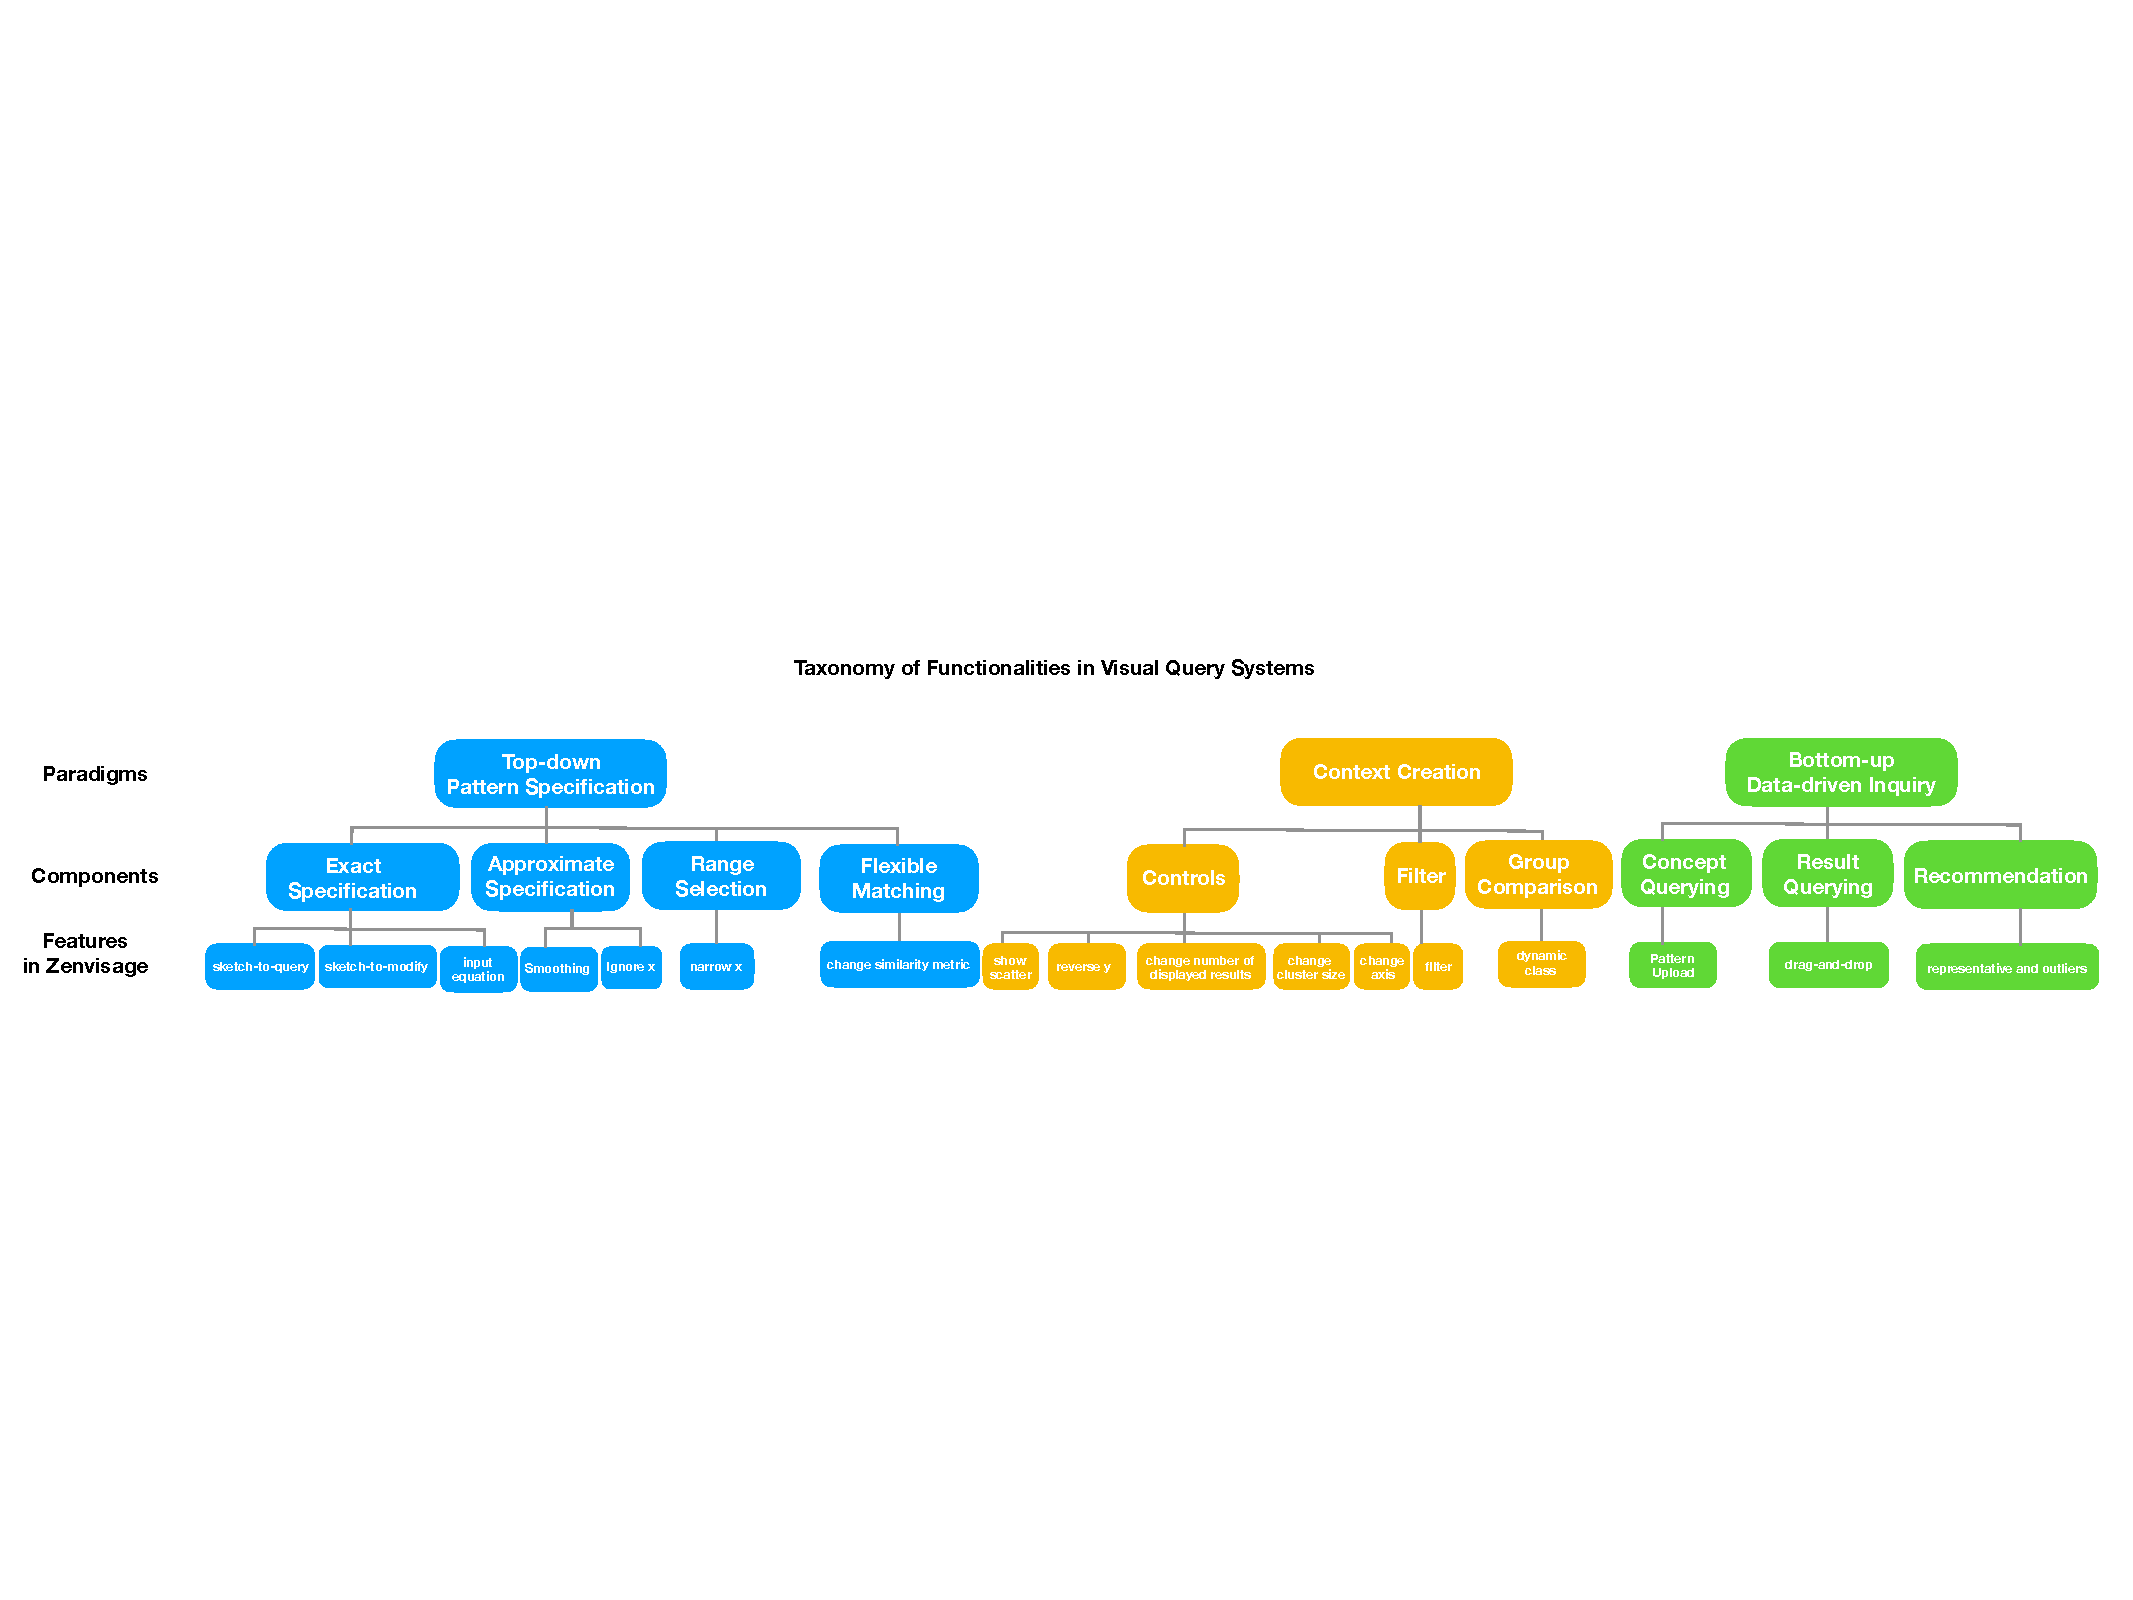
\includegraphics[width=0.9\linewidth]{figures/taxonomy.pdf}
  \caption{Taxonomy of functionalities in VQSs. Each of the three sensemaking process is broken down into key components in VQSs.} %, which is instantiated as features in \zvpp.}% The bottom-most layer connects the use cases features that have practical or envisioned usage based on the evaluation study.}
  \label{fig:taxonomy}
\end{figure*}
\change{
  \subsection{System\label{sec:system}}
  The \zvpp interface is organized into 5 major regions that dynamically updates upon user interactions. Typically, analysts begin their analysis by selecting the dataset and attribute to visualize in the \emph{data selection panel} (Figure~\ref{zvOverview}A). Then, they can specify a pattern query of interest, through either sketching, inputting an equation, uploading a data pattern or dragging and dropping an existing visualization, displayed on the \emph{query canvas} (Figure~\ref{zvOverview}B). \zvpp performs shape-matching between the queried pattern and other possible visualizations and returns a ranked list of visualizations that are most similar to the queried pattern, displayed in the \emph{results panel} (Figure~\ref{zvOverview}C). At any point during the analysis, analysts can adjust various system-level settings through the \emph{control panel} (Figure~\ref{zvOverview}D) or browse through the list of recommendations provided by \zvpp (Figure~\ref{zvOverview}E). Our \zvpp system is open source and available at: \url{github.com/[Annonymized for Submission]}. Given the space limitation of our paper, we have focussed our discussion major \zvpp functionalities relevant to the study findings, and defer the details of other \zvpp features to our technical report~\cite{TR} and documentation in our open-source online repository\footnote{\url{github.com/[Anonymized for Submission]/wiki}}.
}
\subsection{\change{Components} Emerging from Participatory Design\label{sec:pd_findings}}
\change{
  Here, we discuss the purpose of the components in the lower-level of our Figure~\ref{fig:taxonomy} taxonomy, motivating use cases collected over the course of participatory design, and how these themes instantiate into corresponding features in \zvpp and other existing VQSs. Each of the features described (labelled F*) correspond directly to a use case challenge (labelled C*) highlighted in the list above it.
}
% Here, we discuss components
% incorporated in \zvpp, over the course of participatory design, along with similar features in past VQSs.
% that share the same high-level objective.
% \begin{figure*}[ht!]
% \centering
% \vspace{-15pt}
% 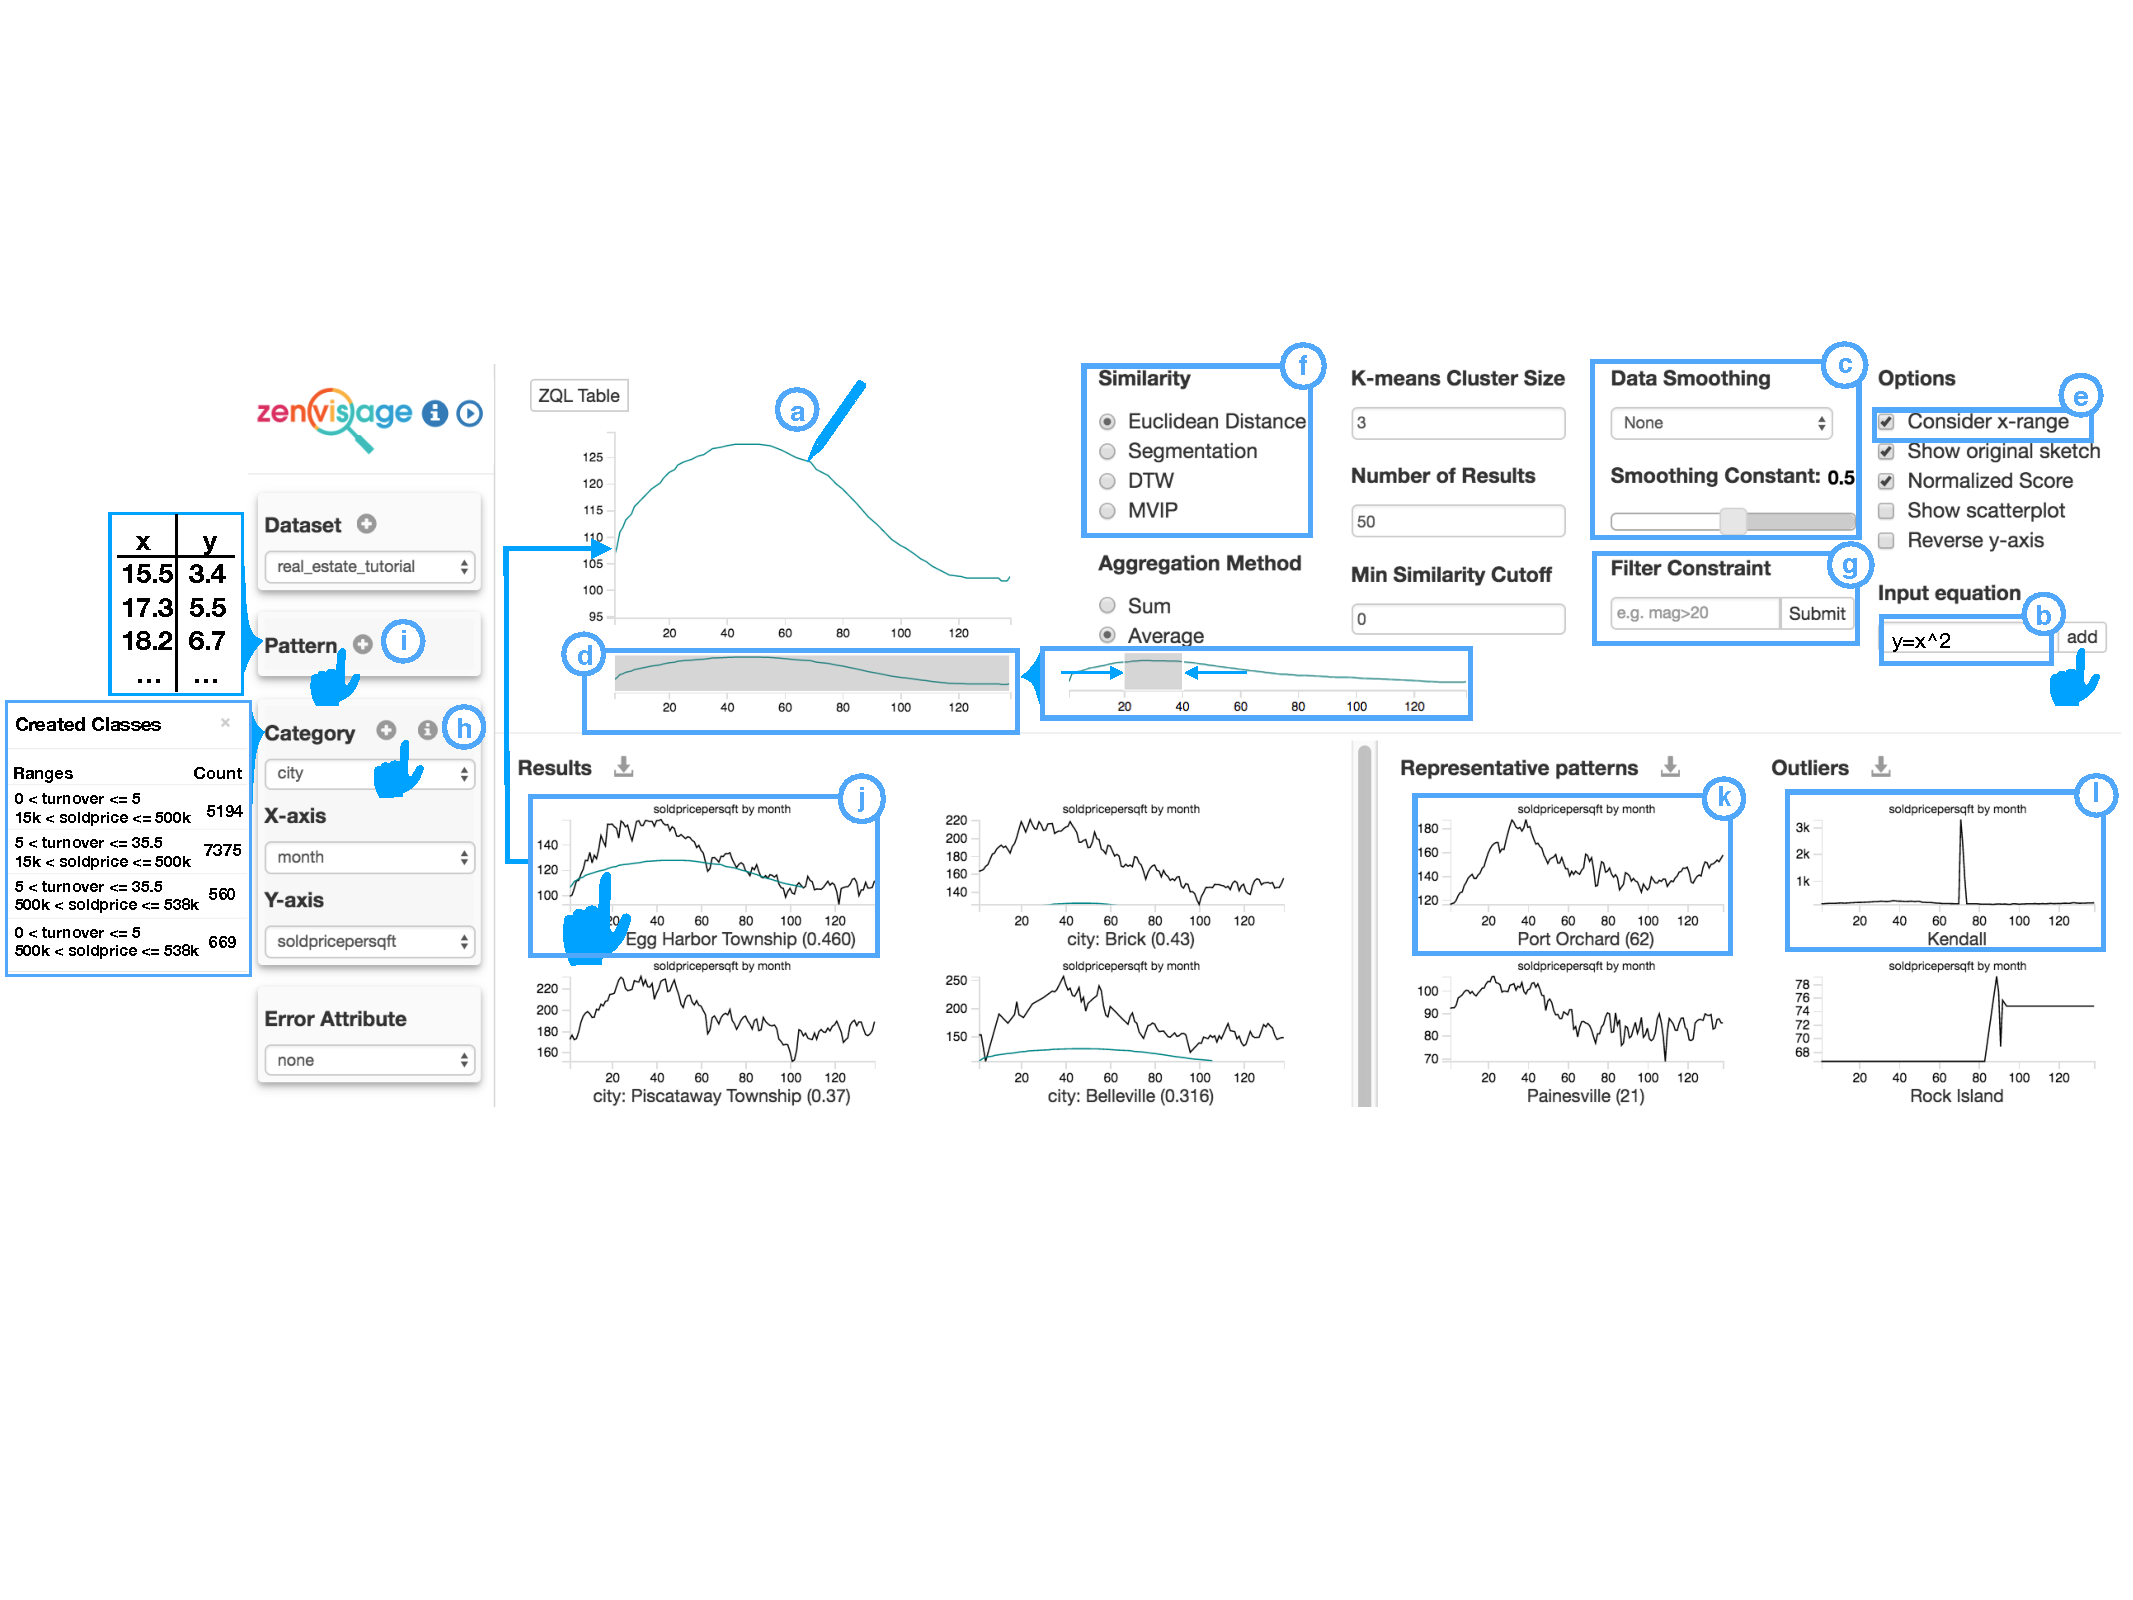
\includegraphics[width=\linewidth]{figures/system.pdf} %5.5
% \vspace{-5pt}\caption{Our VQS after participatory design, which includes: the ability to query via (a) a sketch,(b) input equations, (i) drag and drop, or (j) uploaded patterns; (c) data smoothing; query specification mechanisms including (d) x-range selection and filtering, (e) x-range invariance, (g) filtering, and (h) dynamic class creation; recommendation of (k) representative and (l) outlier trends.} %Prior to the participatory design, \zv only included a single sketch input with no additional options.}
% \label{zvOverview}
% \vspace{-14pt}
% \end{figure*}
 %We discovered three central themes encapsulating these features that are important to facilitate rapid hypothesis generation and insight discovery, but are missing in prior VQSs. While some of our findings echo prior work on system-level taxonomies of visualization tasks \cite{Amar2005,Heer2012}, we highlight how specific analytic tasks and interaction features could be used to enhance VQSs in particular. \techreport{In particular, we learned that \textit{participants wanted more control over the internals of the systems and an integrated workflow that helped streamline their analysis when using VQSs.}}
\change{
  \boldpara{I) Pattern Specification}
  \nstitle{Purpose:} Specify exact descriptions
  of a pattern as a query
  (hereafter referred to as \emph{pattern query}),
  with the VQS returning a list of most similar matches.
  \problemlist
    \item General need for an intuitive mechanism for specifying desired patterns.
    \item Material scientists were interested in finding solvents with known analytical models describing chemical relationships.
    \item Astronomers were interested in specifying the exact width of a supernovae light curve, which is characteristic to the radioactive decay rate of its chemical signature~\cite{Nugent1997}, to distinguish patterns of interest from noise.
  \enumend
  \featurelist
  \item Almost all existing VQSs, including \zvpp, support freehand sketching for specifying a desired query pattern on a virtual canvas (Figure \ref{zvOverview}B1). %\techreport{on a virtual canvas through mouse or pen as a intuitive mechanism }for specifying desired patterns
  %(Figure \ref{zvOverview}a).
  \item The above use cases highlights the common difficulty of sketching precisely. \zvpp allows users to specify a exact functional form (e.g., y=$x^2$) as a pattern query (Figure \ref{zvOverview}D5).
  \item \zvpp also enables users to upload a pattern consisting of a sequence of points as a query (Figure \ref{zvOverview}A1). The pattern upload functionality is also available in Google Correlate~\cite{mohebbi2011google}.l
  \enumend
}
%The uploaded pattern is once again more precise than a sketch.
%For example, , so querying with an exact uploaded pattern would be helpful for distinguishing the patterns of interest from noise.
% The desired patterns uploaded are often generated from computational models or prelabelled data from an external reference database. For example, A1 wanted to query based on synthetic light curves generated from simulations and known supernovae discovered in the past.
% Many participants also envisioned use cases for pattern loading. The ability to load in data patterns as a query would enable users to compare visualizations between different experiments, species, or surveys, query with known patterns from an external reference catalog\techreport{ (e.g. important genes of interest, objects labeled as supernovae)}, or verify the results of a \techreport{simulation or }downstream analysis\techreport{ by finding similar patterns in their existing dataset}. The uploaded pattern also represents a more precise query specification that captures the desired features of a pattern \techreport{(e.g. amplitude, width of peak), }that cannot be precisely sketched. For example, the width of a supernovae light curve is characteristic to the radioactive decay rate of its chemical signature~\cite{Nugent1997}, so querying with an exact pattern template would be helpful for distinguishing the patterns of interest from noise.
% \boldpara{Concept querying} enable users to upload a pattern associated with a concept as a query. As supported in \zv and Google Correlate, users can upload a sequence of points as the query pattern (Figure \ref{zvOverview}i). This is useful for patterns generated from computational models or prelabelled data from an external reference database. For example, A1 wanted to query based on synthetic light curves generated from simulations and known supernovae that have been discovered in the past.
%While pattern specification is an intuitive mechanism for constructing a visual query, p
\change{
  \boldpara{II) Match Specification}
  \nstitle{Purpose:} Past work has shown that pattern queries can be imprecise~\cite{correll2016semantics,Holz2009,Eichmann2015}. To this end, VQSs need to support mechanisms for clarifying the interpretation of the sketch (i.e., how matching should be performed).
  \problemlist
    \item Dense and noisy observational data in astronomy and material science makes it difficult to match with other patterns exactly.
    \item When analyzing line charts, there are often specific ranges with domain significance that users want to restrict their search within or outside of these ranges (e.g., a known period of time when an imaging equipment is malfunctioning).
    \item Astronomers and geneticists were interested in qualitative patterns, such as the existence of a peak above a certain amplitude or a `generally rising' profile, without regards to the exact time when the event occurs. The default Euclidean metric unnecessarily penalizes unaligned time-series of interest.
  \enumend
  \featurelist
  \item \zvpp supports an interface for users to adjust smoothing algorithms and parameters on-the-fly to update the resulting visualizations accordingly (Figure \ref{zvOverview}D2). In addition to denoising the data, data smoothing effectively allows users to change the degree of shape approximation they would like to apply to all visualizations when performing pattern matching. Smoothing is also supported in Qetch~\cite{Mannino2018}. Other interfaces have also developed constrained sketching mechanisms to allow users to partially specify certain shape characteristics, such as angular slope queries\techreport{for specifying the slope of a trend line}~\cite{Hochheiser2004} or piecewise trend querylines\techreport{over a specified data range}~\cite{ryall2005querylines}. Smoothing was chosen over these other interfaces for approximating key patterns in the data, since it was a familiar preprocessing step in our study participants' workflow.
  \item To restricted search to selected ranges in \zvpp, users can select desired x-ranges to perform matching through brushing interactions (Figure \ref{zvOverview}B2) or enter a y-range selection in the filter constraint textbox (Figure \ref{zvOverview}D4). Other interfaces for range selection in past VQSs
  include textboxes~\cite{wattenberg2001sketching,Mannino2018}, min/max line boundaries~\cite{ryall2005querylines},
  or brushing interactions~\cite{Hochheiser2001}. TimeSearcher and Queryline's approach is most flexible for range selection as
  they allow composition of multiple ranges to formulate complex piecewise queries, such as finding gene expression profiles
  rising from x=1-5 then declining from x=5-10. Inspired by TimeSearcher's brushing interaction, we support only brushing for x, since in most of our use cases it was more common to focus the context based on the independent variable, such as zooming into particular sharp dips when looking for planetary transits or anomalous peaks indicative of erroneous experimental measurements.
  %\agp{Again, why did we pick ours then?If ours is similar to Hochheiser, we can saythat we used that as inspiration to build ours.} %Additionally, y axis range selection could be performed through entering a filter constraint on the measure variable.
  \item  In addition to controls for fine-tuning the portions of the sketch to be matched, VQSs also need to allow users to control the underlying matching algorithm. In \zvpp, users have the option to change similarity metrics to perform flexible matching (Figure \ref{zvOverview}D1). \zvpp supports an option to ignore the x-range in shape matching (Figure \ref{zvOverview}D4). This feature is similar to `temporal invariants' in SketchQuery~\cite{correll2016semantics}.
  \enumend
}
%For finding supernovae, A1 primarily cared about the existence of a peak\techreport{above a certain amplitude with an appropriate width of the curve}, rather than the exact time that the event occurred. G1 also expressed that she does not care about when the `trigger point' occurs as long as the profile is rising.
% \techreport{\par During participatory design, both material science and astronomy participants noted the difficulty of shape matching on their dense and noisy observational data and the challenge of picking the appropriate smoothing parameters during offline preprocessing. We found that tight integration between smoothing and visual search additionally tradeoff between the smoothness of the curve and the degree of approximation for shape-matching in VQSs. An over-smoothed visualization would return shape matches that only loosely resemble the query pattern. However, without smoothing, the noise may dominate the overall trend, which could lead to bad pattern matches.}
%While the interactions in our original prototype enabled simple visual queries, many scientists were interested in extending their querying capabilities, either through different querying modalities or through more flexible query specification methods.
% While \zv does not attempt to solve all of the pre-processing issues that we faced during participatory design, we identified data smoothing as a common data cleaning procedure that could benefit from a tight integration between pre-processing and visual analysis. Data smoothing is a denoising procedure that generates a smoothed pattern approximating key features of the visualized trend with less noise.
% \boldpara{Range Selection:} Often in time series analysis there are specific ranges of time and measure values with special domain specific significance that may be of interest to users. To find such patterns, users can limit the pattern query to be matched only in specific x or y ranges, specified through textboxes~\cite{wattenberg2001sketching,Mannino2018}, min/max line boundaries~\cite{ryall2005querylines}, or brushing interactions~\cite{Hochheiser2001}. \zv employs the brushing mechanism to select desirable x-ranges to perform shape matching (Figure \ref{zvOverview}d). Additionally, y axis range selection could be performed through entering a filter constraint on the measure variable.
% \par We chose to support only brushing for x, since it was more common to focus the context based on the independent variable in our use cases, such as zooming into particular sharp dips when looking for planetary transits or anomalous peaks indicative of erroneous experimental measurements. \cut{In contrast, y-range selection tends to be more global and enforced across multiple interaction sequences, such as looking for only signals above a certain threshold.} The TimeSearcher and Queryline approach is most flexible as they allow composition of multiple range selections to formulate complex piecewise queries, such as finding gene expression profiles rising from x=1-5 then declining from x=5-10.
% \boldpara{Flexible Matching:}
%Studies have shown that \techreport{to facilitate subjectively meaningful pattern matches,} VQSs need to support mechanisms for clarifying sketch interpretation and flexible shape matching algorithms~\cite{correll2016semantics,Mannino2018,Eichmann2015}.
% This latter features is akin to the temporal invariants in SketchQuery.
\change{
  \boldpara{III) View specification}
  \nstitle{Purpose:} Modify visualization settings for all visualizations displayed on the VQS. The ability to change the view specification offers analysts different perspectives on the same portion of data.
  \problemlist
    \item For non-time-series uses of VQS, such as in material science, analysts is often interested in pivoting across various different x and y axes attributes.
    \item Astronomers often view magnitude measurements by reversing the y-axes, material scientist often prefer viewing their data in terms of a scatterplot rather than line charts.
  \enumend
  \featurelist
    \item The data selection panel in \zvpp allows users to select dataset and attributes of interest.
    \item Display options can be modified via the control panel in \zvpp, such as reversing the y axes or changing visualization mark type to scatter.
  \enumend
}
\change{
  \boldpara{IV) Slice-and-Dice}
  \nstitle{Purpose:} Navigate and compare collections of visualizations constructed from different portions of the data.
  \problemlist
    \item Since astronomers often have datasets with large numbers of objects, they first use domain knowledge
    to narrow down their search to a more manageable subset to increase their chances of finding an interesting pattern for a given pattern query.
    \item Material scientists often partition solvent datapoints into customized classes based on their physical properties, in order to compare between these classes. For example, M1 wanted to create classes of solvents with ionization potential under -10 kJ/mol, over -8 kJ/mol, and ones between that range, and examine how visualizations involving lithium solvation energy varied across the three classes.
  \enumend
  \featurelist
    \item To filter data on-the-fly in \zvpp, users can compose one or more conditions as filter constraints in a textbox (Figure \ref{zvOverview}D3). The filtering can be done on data columns associated with each pattern that is not visualized or on the visualized attributes. This feature is unique to \zvpp as most existing VQSs do not allow users to interact with data in the non-visualized columns.
    \item \zvpp supports dynamic class creation, a feature that allows users to create custom classes interactively,
    based on multiple data properties, following which each class can be visualized as a separate visualization (Figure~\ref{dcc}). Information regarding the created classes is displayed in a table and as a tooltip over the aggregate visualizations.
    \begin{figure}[h!]
      \centering
      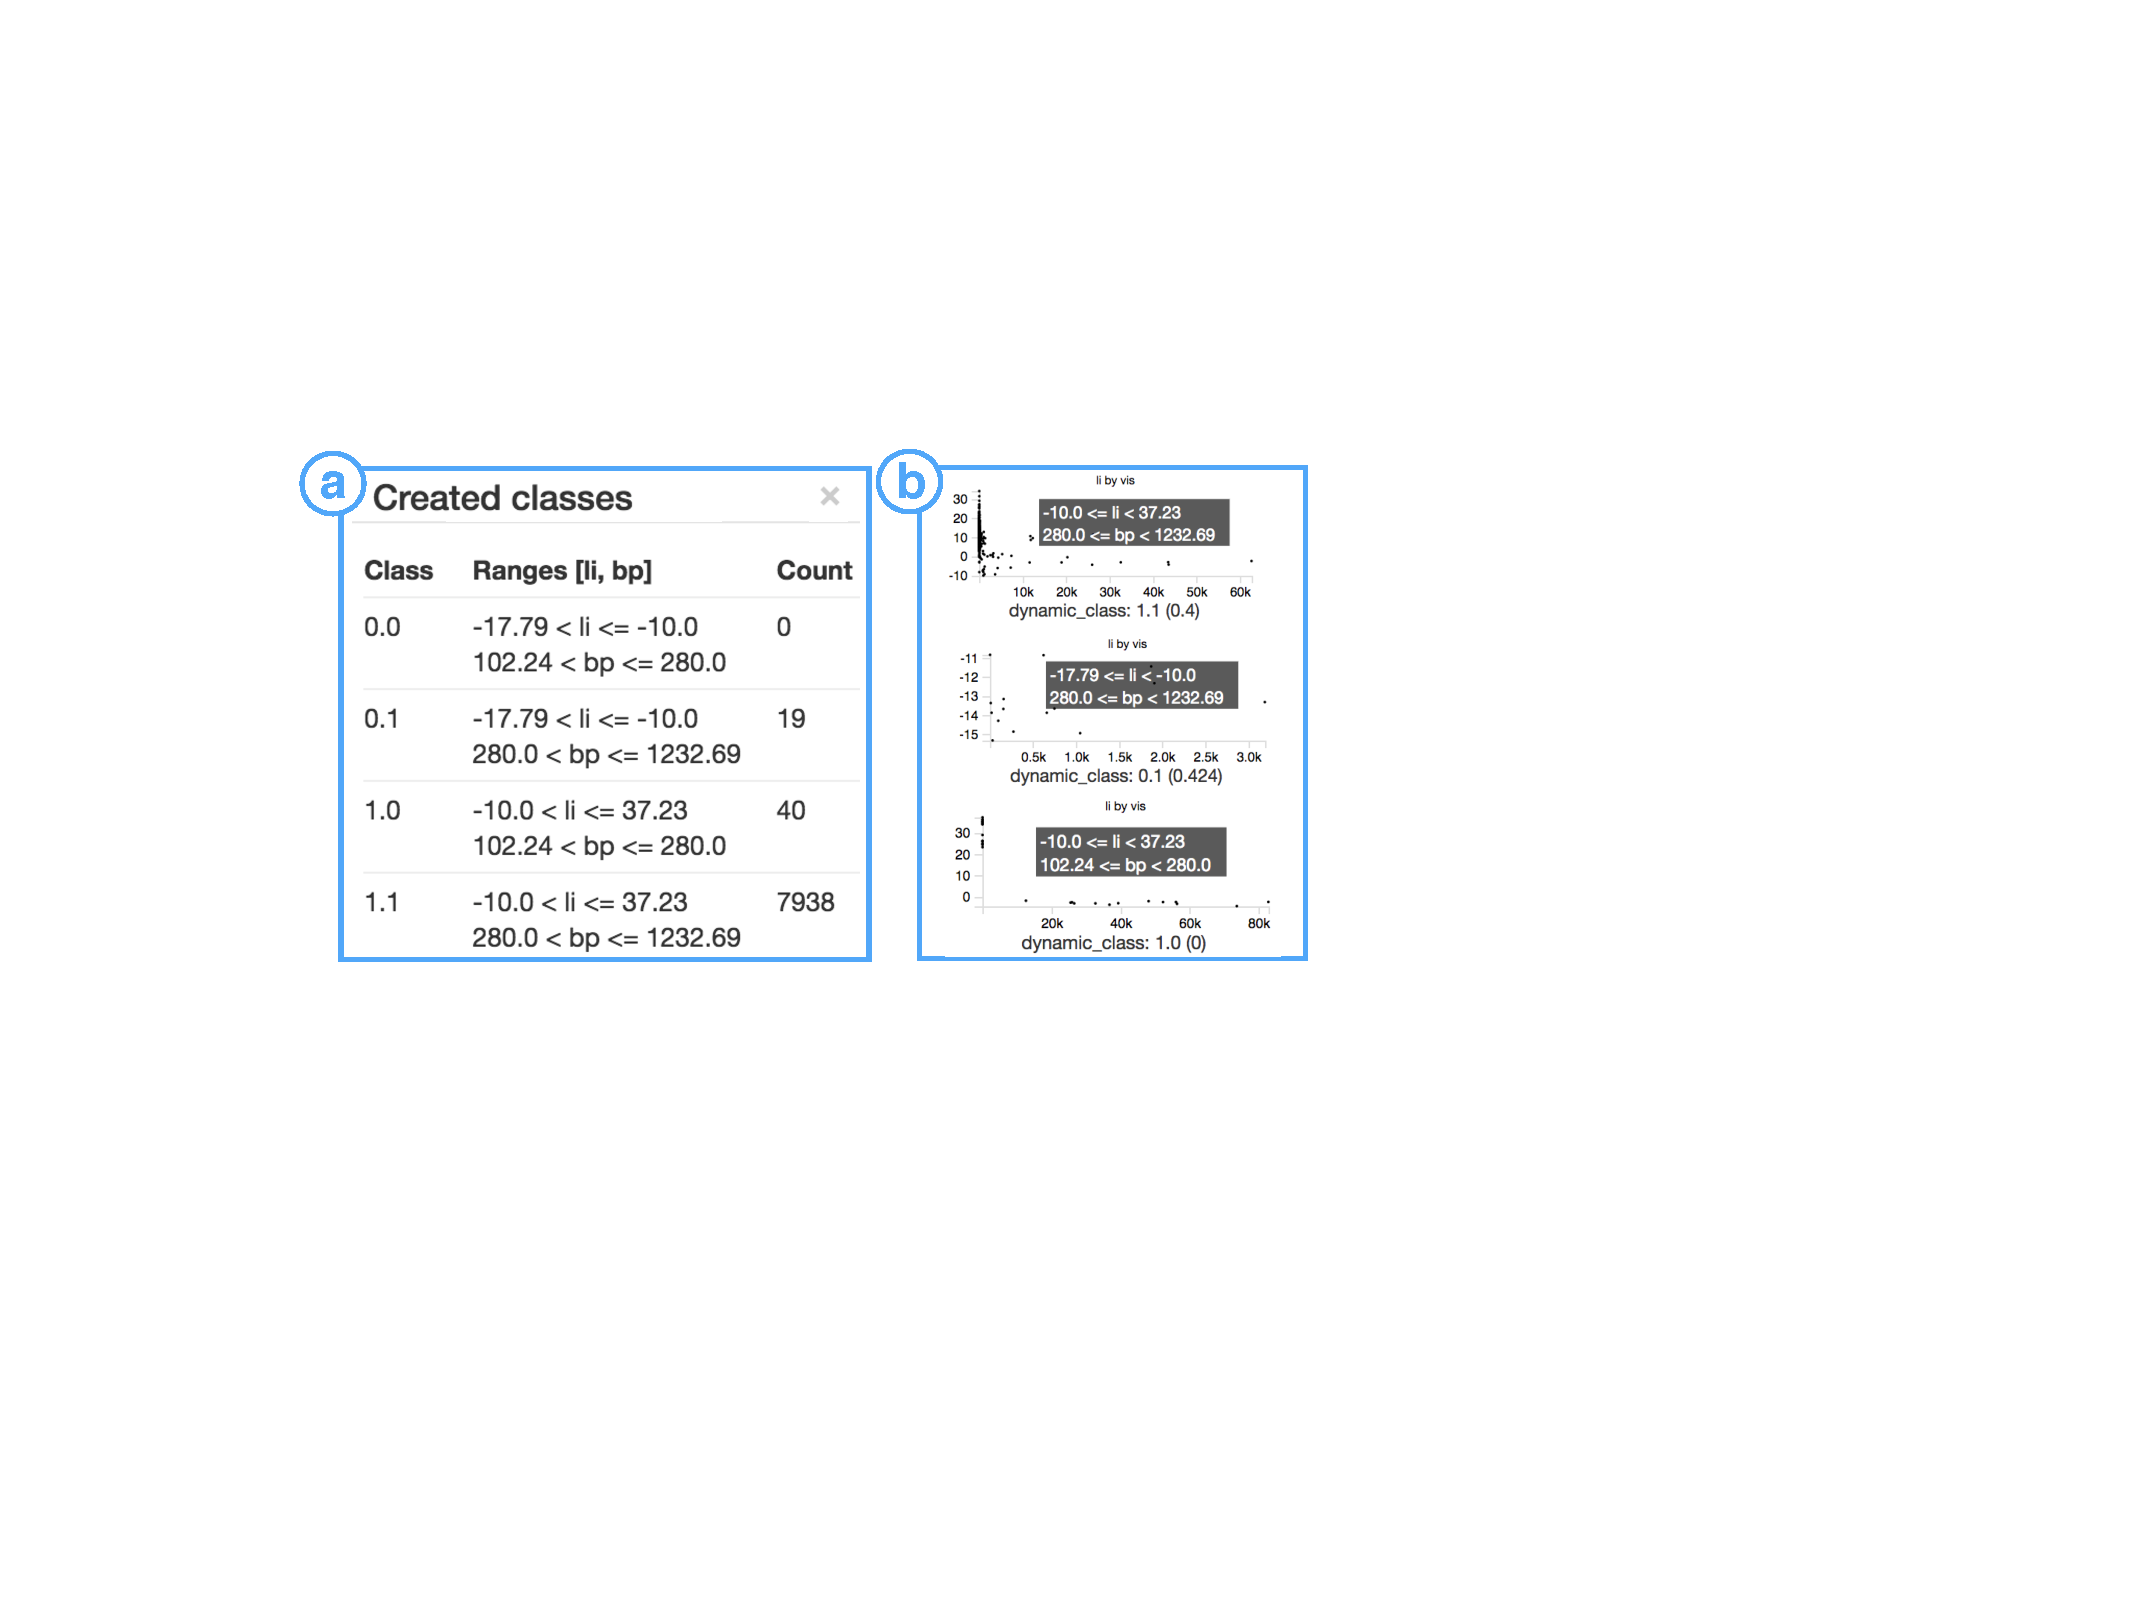
\includegraphics[width=0.95\linewidth]{figures/dcc.pdf}
      \vspace{-6pt}
      \caption{\change{Example of dynamic classes. (a) Four different classes with different Lithium solvation energies (li) and boiling point (bp) attributes based on user-defined data ranges. (b) Users can hover over the visualizations for each dynamic class to see the corresponding attribute ranges for each class. The visualizations of dynamic classes are aggregate across all the visualizations that lie in that class based on the user-selected aggregation method.}}
      \label{dcc}
      \vspace{-10pt}
    \end{figure}
  \enumend
}
%We designed two dynamic faceting features coupled with coordinated views that enabled users to specify subsets of data they are querying on and see immediate changes updated in the query, representative, and outlier results.
%\boldpara{Group Comparison} addresses a common analytical task where users want to
% , as shown in Figure~\ref{dcc}.
%While input equations are useful when simple analytical models exist, this may not be true for other domains. In these scenarios, users can upload a query pattern of a sequence of points
 %Similarly, Google Correlate allows users to upload their own time series or enter search keywords that corresponds to a time series.
%, usually as part of the downstream analysis of the exploratory workflow. %For example, the genetics team are trying to develop a time series prediction algorithm using machine learning based on some biological parameters \cite{Peng2016}.
\change{
  \boldpara{V) Result querying}
  \nstitle{Purpose:} Querying based on the displayed results (either from the ranked list in Figure~\ref{zvOverview}C or recommendations from Figure~\ref{zvOverview}E), essentially requesting for patterns similar to the selected data pattern.
  \problemlist
    \item General need for having to search for a pattern similar to a visualization of interest. For example, G1 was interested in the gene `Esrrb' and wanted to find other genes that exhibits a similar pattern to it.
  \enumend
  \featurelist
    \item In \zvpp, users can drag and drop a visualization in either the results pane or the representative and outliers to the query canvas (Figure \ref{zvOverview}j). Similarly, TimeSearcher enable users to instantiate queries via drag-and-drop, whereas QuerySketch does so through double clicking.
  \enumend
  \boldpara{VI) Recommendation}
  \nstitle{Purpose:} displays visualizations that may be of interest to the users based on the data context.
  \problemlist
    \item Geneticists are often interested in learning about the common gene expression profiles in their dataset.
  \enumend
  \featurelist
    \item \zvpp provides visualizations of representative trends based on clustering and highlights outlier instances\techreport{ that look different from the rest of the visualizations} (Figure \ref{zvOverview}E).%The recommendation feature is unique to \zv, which provides visualizations of representative trends based on clustering and highlights outlier instances that looks different from the rest of the visualizations (Figure \ref{zvOverview}k,l).
  \enumend
}
% In this section, we first describe a model to help characterize the design space for VQS based on the analytical workload and usage patterns from different use cases. Then, we present design challenges related to each of the process.
\begin{table}
		\centering
    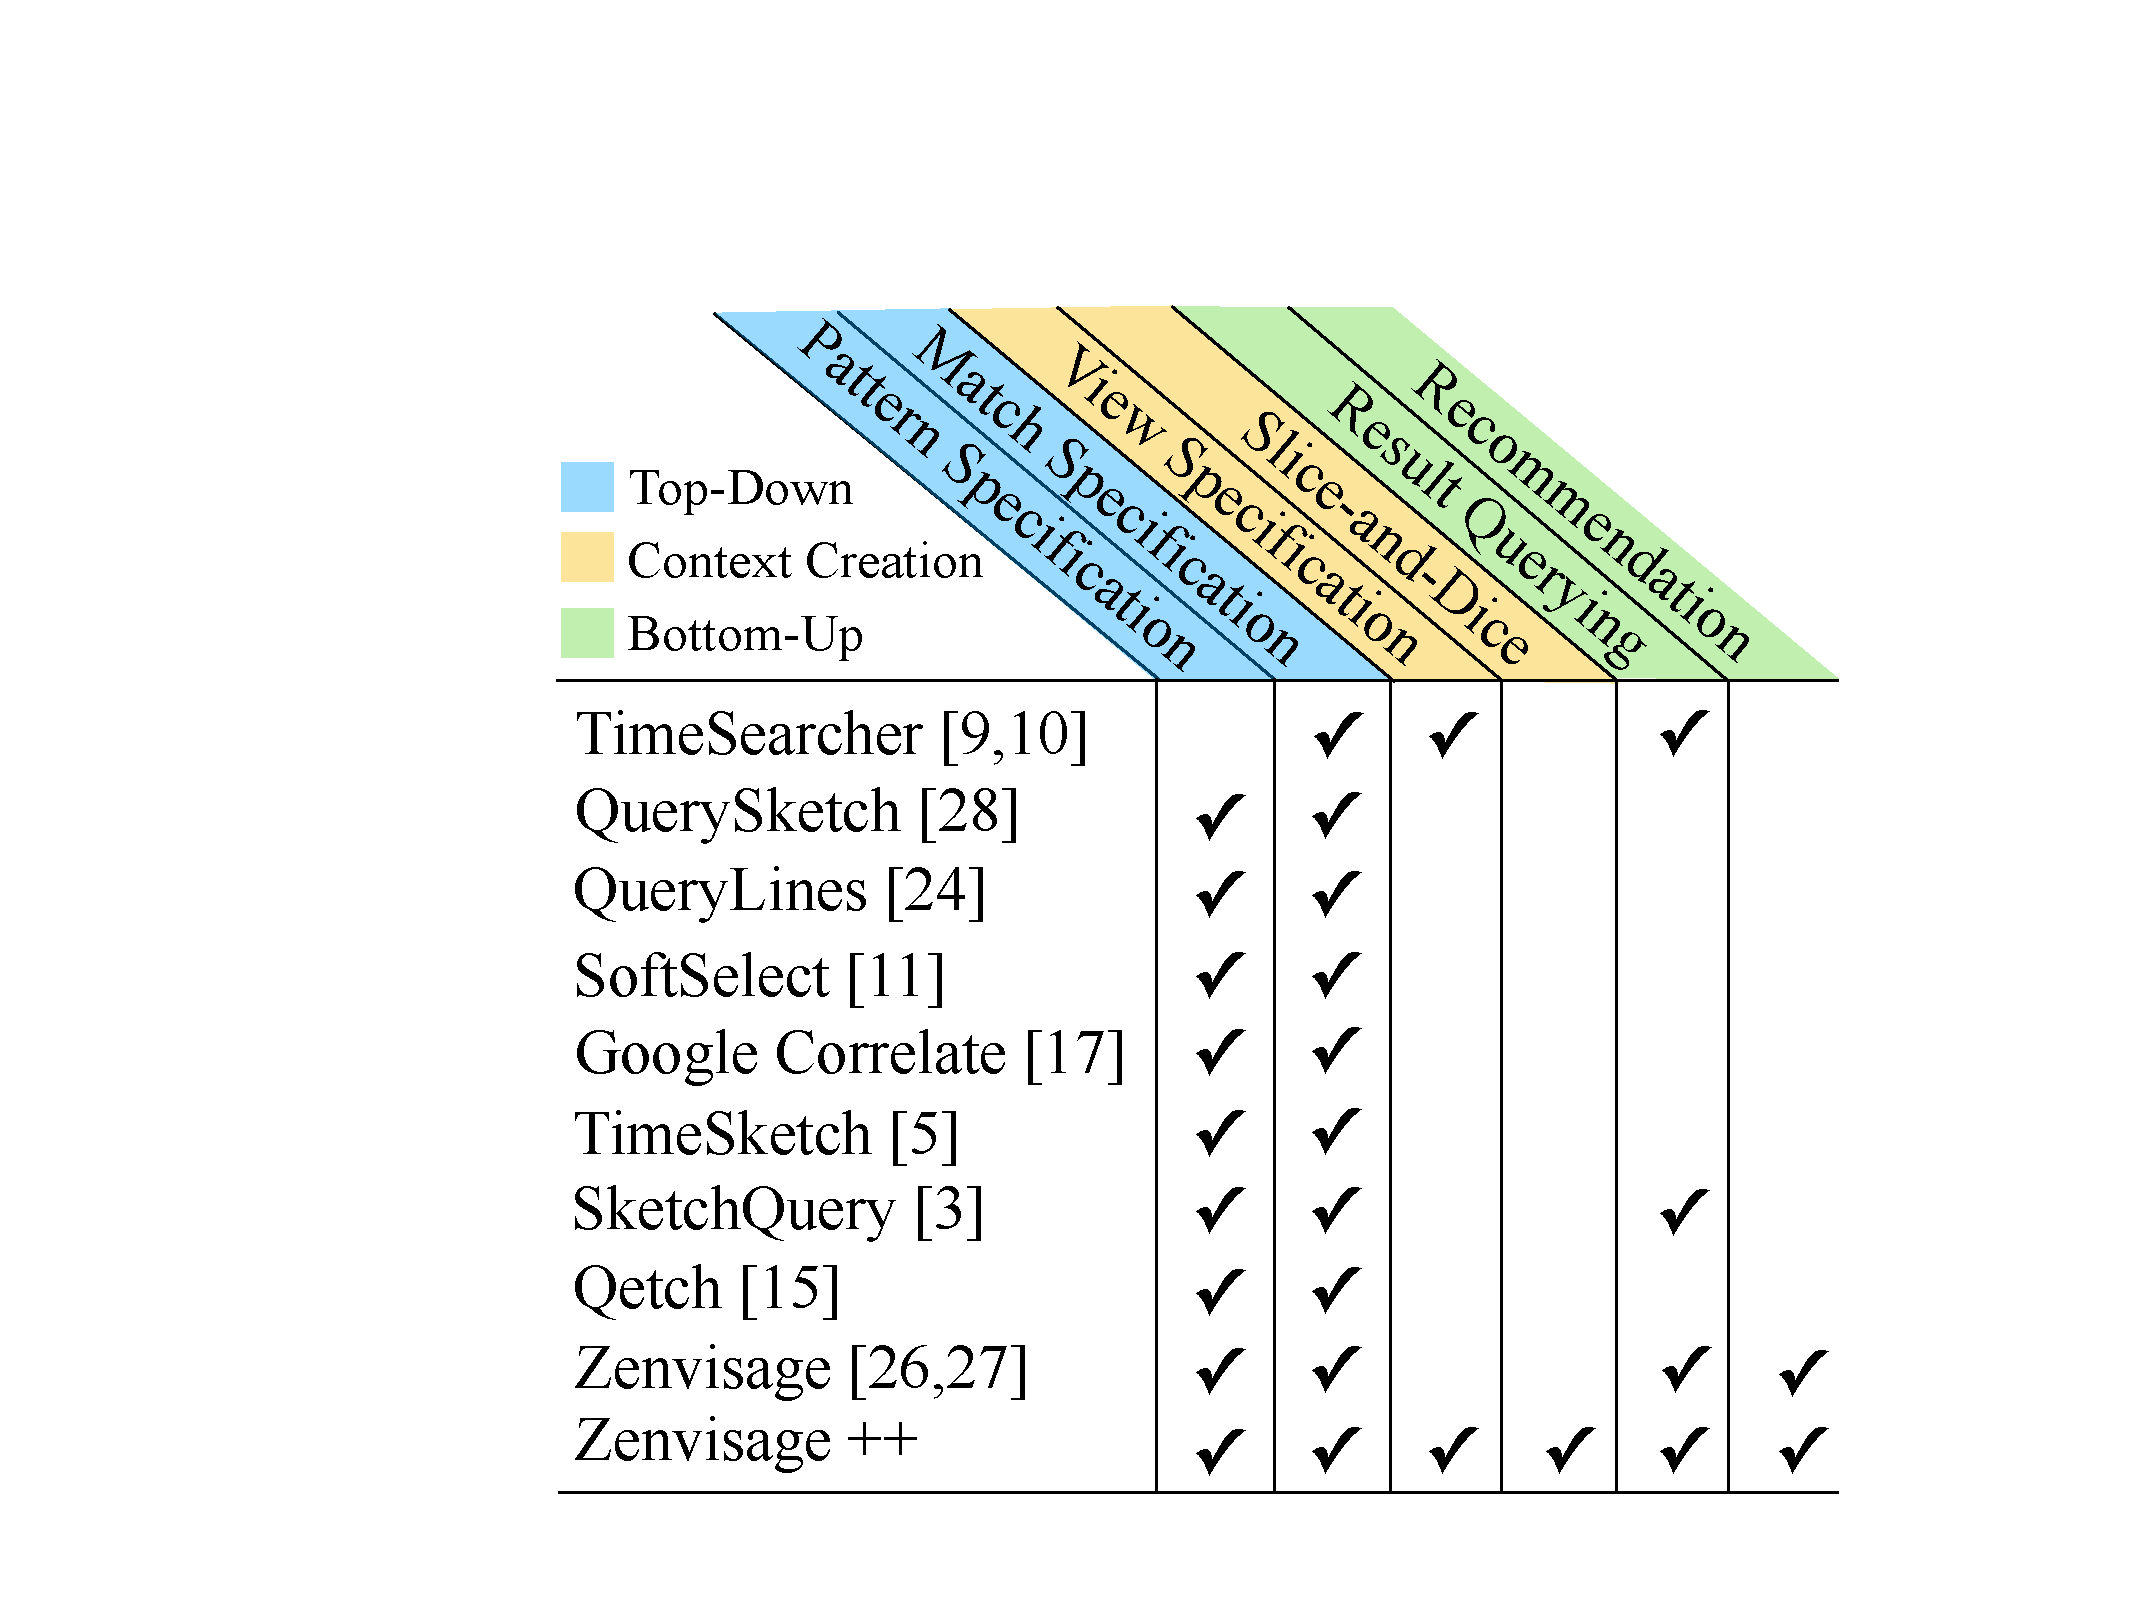
\includegraphics[width=0.8\linewidth]{figures/related_works_table.pdf}
    \caption{Table summarizing whether key functionalities of VQSs (columns) are covered by past systems (row), indicated by checked cells. Column header colors blue, orange, green represents three sensemaking process (top-down querying, search with context, and bottom-up querying)\cut{ described in Section~\ref{sec:pd_findings}}. The heavily-used, practical features in our study for context-creation and bottom-up inquiry is largely missing from prior VQSs.}
    \label{table:relatedwork}
    \vspace{-10pt}
\end{table}
\subsection{Characterizing the Problem Space for VQSs}
%Based on example use cases and feature components from participatory design, we further characterize the design space of VQSs. further characterize three sensemaking process within the problem space of VQSs.
Given our earlier description of VQS features organized into components, we now introduce the three sensemaking processes by characterizing how they fit into different problem areas that VQSs are aimed to solve. Visual querying often consists of searching for a desired pattern instance (Z) across a visualization collection specified by some given attributes (X,Y). \change{Correspondingly, }we introduce two axes depicting the amount of information known about the visualized attribute and pattern instance.%, as shown in Figure~\ref{2dmodel}.
%(e.g., only interested in patterns related to a specific gene)
\par Along the \textbf{pattern instance} axis,
the visualization that contains
the desired pattern may already be \texttt{known} to the analyst,
exist as a pattern \texttt{in-the-head} of the analyst,
or completely \texttt{unknown} to the analyst.
In the \texttt{known} pattern instance region (Figure~\ref{2dmodel} grey), visualization-at-a-time
s such as Tableau,
where analyst manually create and examine each visualization one at a time,
is more well-suited than VQSs, since analysts can directly work with the selected instance without the need for visual querying.
Inspired by Pirolli and Card's information
foraging framework~\cite{Pirolli}, which distinguishes
between information processing tasks that are \textit{top-down}
(from theory to data) and \textit{bottom-up} (from data to theory),
we define \textit{top-down pattern specification} as the search-oriented paradigm where analysts query based on their
in-the-head pattern (Figure~\ref{2dmodel} blue) in a fixed collection.
On the other hand, in the realm of \textit{bottom-up
data-driven inquiry} (Figure~\ref{2dmodel} green),
the pattern of interest is unknown and external
to the user and must be driven by recommendations
or queries that originate from the data (or equivalently, the visualization).
As we will discuss later, this process is crucial
but underexplored in past work on VQSs.
%analysts often do not start with a known pattern instance. T
\par The second axis, \textbf{visualized attributes},
depicts how much the analyst
knows about which X and Y axes
they are interested in visualizing.
In both the astronomy and genetics use cases,
as well as past work in this space,
data was in the form of a time series
with \texttt{known} visualized attributes.
In the case of our material science participants,
they wanted to explore relationships between different
X and Y variables.
In this realm of \texttt{unknown} attributes,
context creation (Figure~\ref{2dmodel} yellow)---i.e.,
setting the stage for bottom-up or top-down processes---\dor{this clause is awkward?}is
essential for allowing users
to pivot across different visualization collections.%subspaces. %Most past VQSs assume that the analyst has a desired pattern in-the-head that could be conveyed through visual specification, such as a sketch.
\begin{figure}[h!]
  \centering
  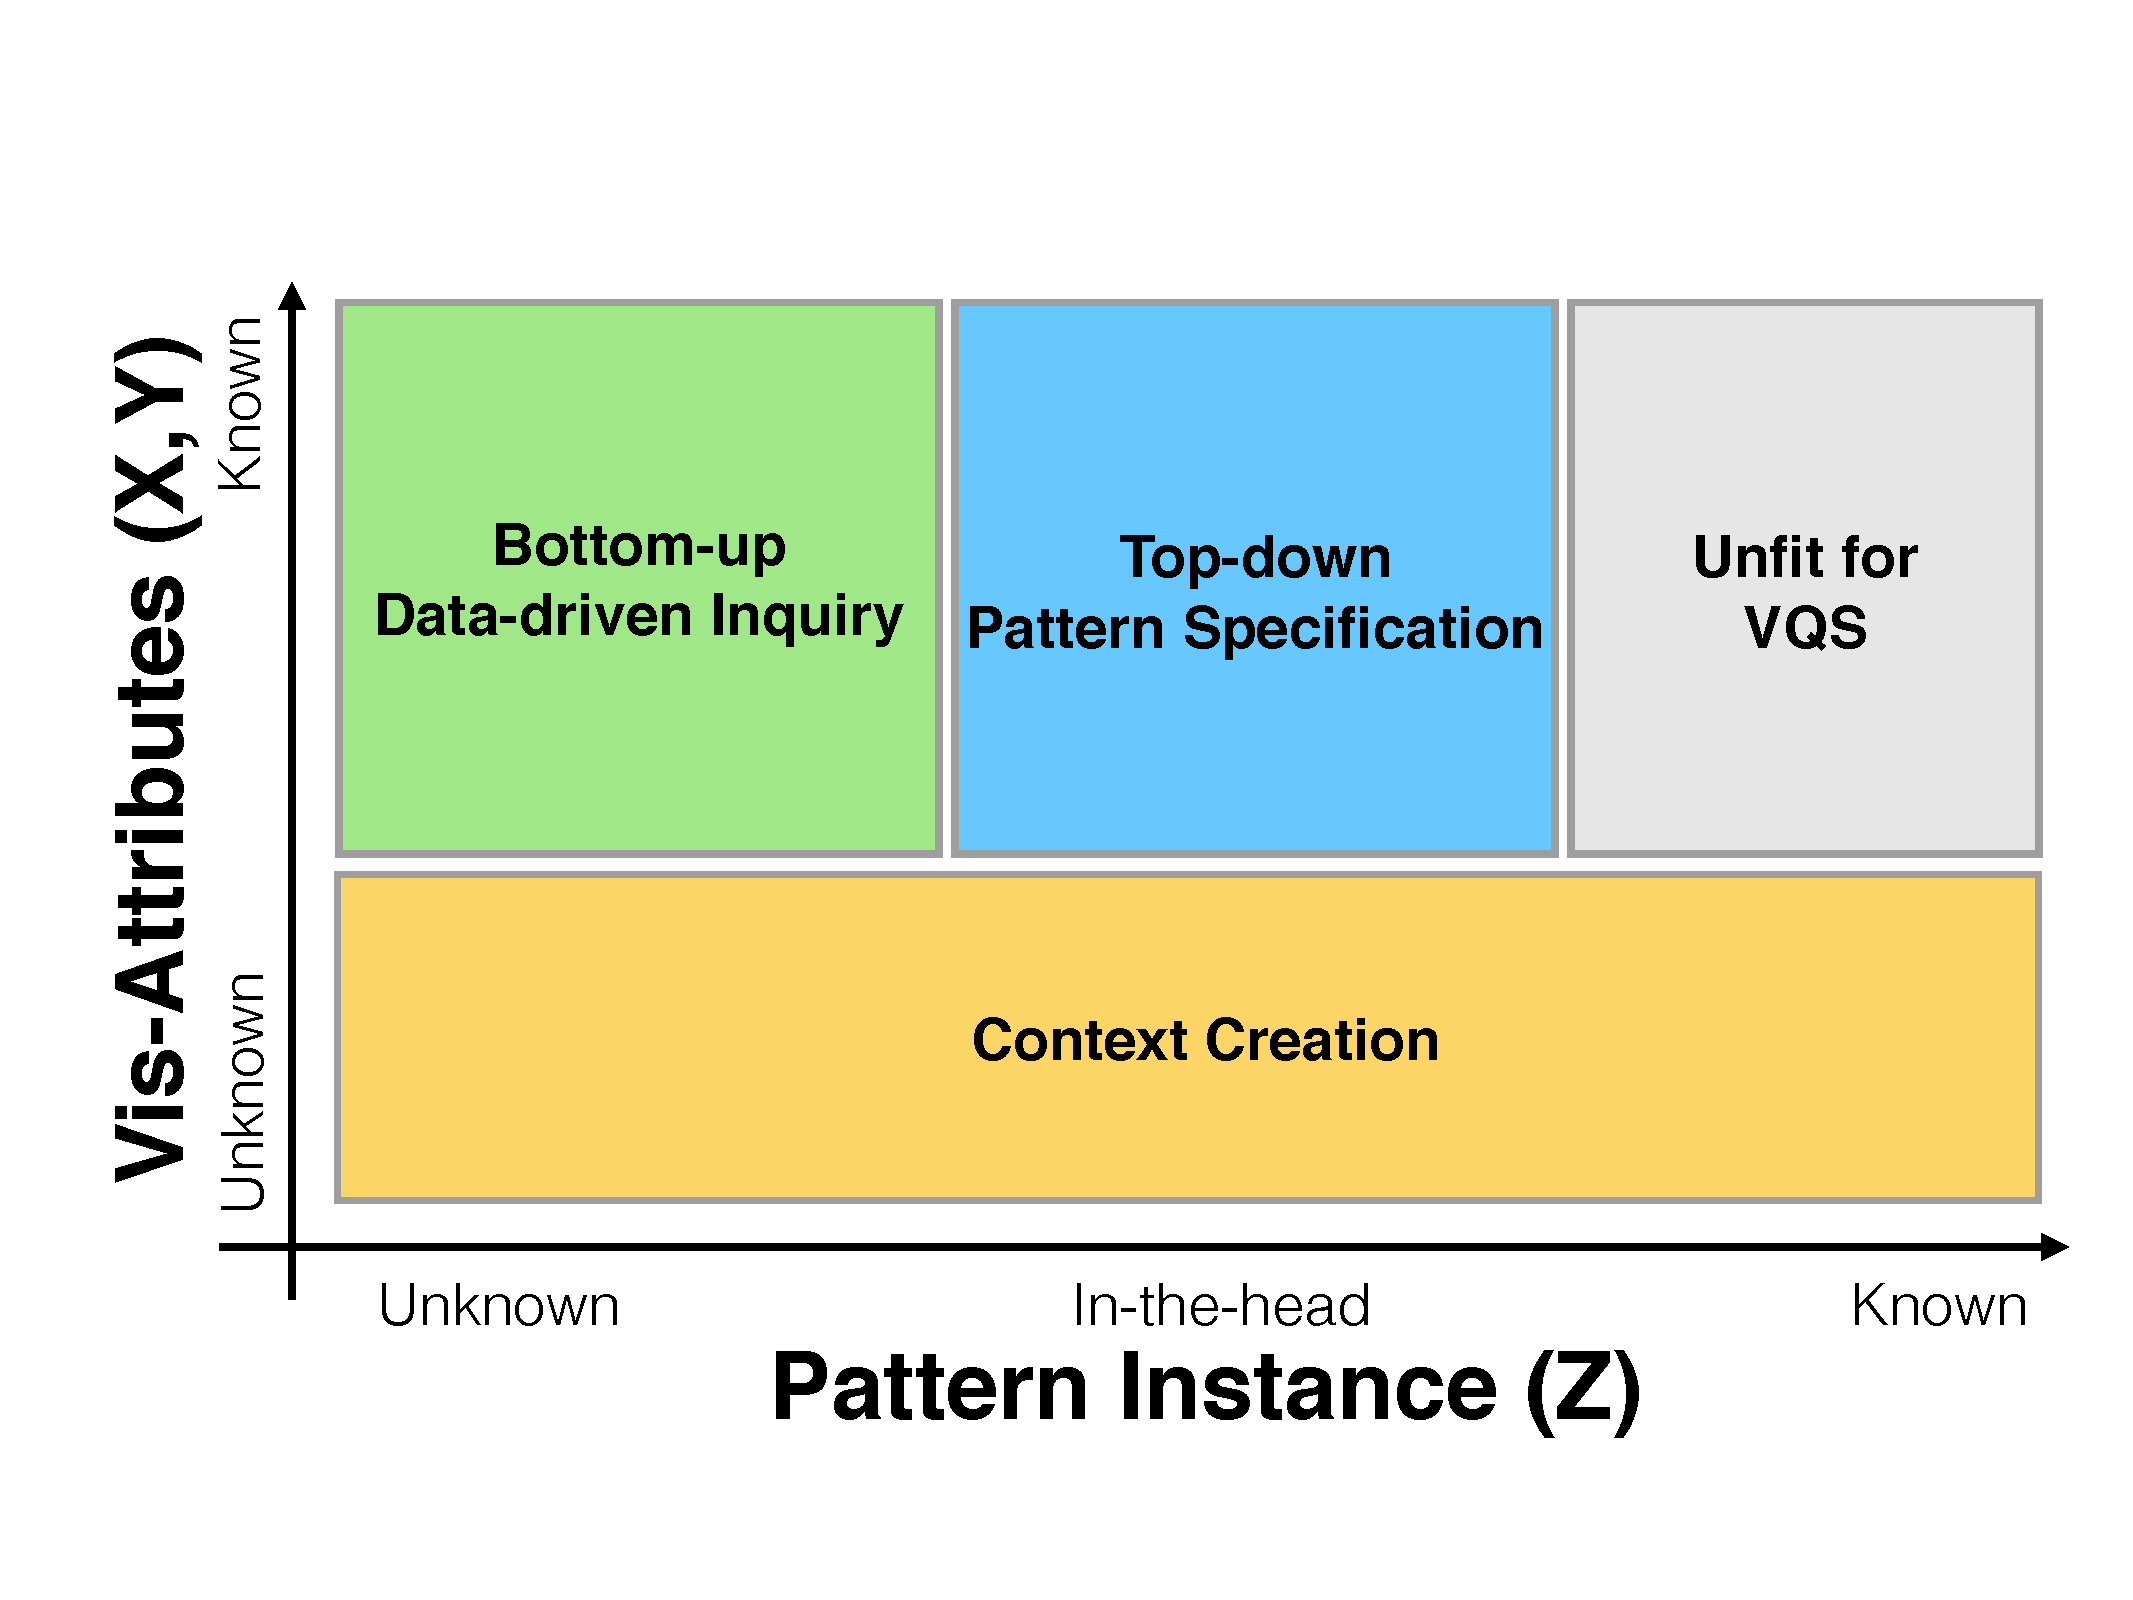
\includegraphics[width=0.9\linewidth]{figures/2dmodel.pdf}
  \caption{The problem space for VQSs is characterized by how much the analyst knows about the visualized attributes and the pattern instance. Colored areas highlight the three sensemaking processes in VQSs for addressing these characteristic problems. While prior work has focused solely on use cases in the blue region, we envision opportunities for VQSs beyond this to a larger space of use cases covered by the yellow and green regions.}
  \label{2dmodel}
  \vspace{-10pt}
\end{figure}
\subsection{Design Goals for the Sensemaking Processes}
After understanding how each sensemaking process fits into the problem space addressed by VQSs, we further explore the design objectives and challenges in supporting each sensemaking process, grounded in our collaborative design experience. % based on the taxonomy orgaby developing a taxonomy for organizing the aforementioned components.% fits into the paradigms of sensemaking in VQSs, as shown in Figure~\ref{fig:taxonomy}. In particular, we will describe the main form of inquiry addressed by each paradigm\cut{(\textit{what, where, which})}, its characteristic use case, and design challenges in supporting these paradigms.
% \par Drawing from our participatory design experience, evaluation study, and literature review in this space, we design a taxonomy for understanding the key functionalities in VQSs. In Figure~\ref{fig:taxonomy}, we show how each use cases makes use of the different features in \zv, then we organize the features into key components for VQSs, which belongs to one of the three paradigms in the VQS design space.%, effectively moving rightwards to the gray area in Figure~\ref{2dmodel}, where the pattern instance is known.
\boldpara{Top-down Pattern Specification} begins with the user's intuition
about how their desired patterns should look like based on `theory', including visualizations from past experience or abstract conceptions based on external knowledge. The goal of top-down pattern specification is to address the \textit{which} question of visual sensemaking: \textit{which pattern instance exhibits this pattern?} Based on this preconceived notion of what to search for, the design challenge is to translate the query in the
analyst's head to a query executable by the VQS.
In the taxonomy in Figure~\ref{fig:taxonomy},
this includes both components for specifying the pattern,
as well as controls governing the underlying
algorithm of how shape-matching is performed.
For example, A1 knows intuitively
what a supernovae pattern looks like
and the detailed constraints on the shape,
such as the width and height of the peak
or the level of error tolerance for defining a match.
He can search for transient patterns through sketching,
select the option to ignore differences
on the x axis, and changes the similarity metric for flexible matching.  %The design challenge of top-down pattern specification is to ----- enable users to How to translate the in-the-head query to visual query and how matching is done.
\boldpara{Bottom-up data-driven inquiry} is
a browsing-oriented sensemaking process
that goes from data to theory to
addresses the \textit{what} questions
in the sensemaking process.
% While the usage of each querying feature may vary from one participant to the next, generally, result querying and pattern upload are considered bottom-up approaches that go from data to theory by enabling users to query via examples of known visualizations. Bottom-up data-driven inquiries
 For example, genetics participants do not
 have a preconceived knowledge of what to search
 for in the dataset.
 They were mostly interested in
 \textit{what types of patterns exist in the dataset}
 through representative trends, as a means to
 jumpstart further queries. %The goal of data-driven inquiry is to move towards the blue area in Figure~\ref{2dmodel} to help analysts gain more information about patterns of interest in-the-head.
% notion of what the pattern looks like
The design challenge include developing
the right set of `stimuli' that could
provoke further data-driven inquiries,
as well as low-effort mechanisms to search via these results.
\boldpara{Context Creation} addresses the \textit{where}
question of sensemaking by enabling analysts
to navigate across different parts of the visualization
collection to learn about \textit{where the patterns of interest lie}.
For example, material scientists often do not start
with a pattern in-the-head, but recognize salient
trends such as inverse correlation or linear correlation.
They switch between different visualized attributes or dynamic
classes to study their data from alternative perspectives.
The design challenge of context creation is to develop
features that act as a `lens': navigating users to desired data subsets,
visualizing and comparing how the data changes between the different lenses, and ensuring that context is dynamically reflected across other VQS functionalities.
\par\noindent The three aforementioned sensemaking processes are akin to the well-studied sensemaking paradigms of search, browse, and faceted navigation on the Web~\cite{Hearst2009,Olston2003}. Due to each of their advantages and limitations given different information seeking tasks, search interfaces have been designed to support all three complementary acts and transition smoothly between them to combine the strength of all three paradigms. \change{Similarly for VQSs, our main design objective in developing \zvpp is to integrate all the three sensemaking in the same system. As we discover in the evaluation study in the following section, this integration encourages and accelerate the process of visualization discovery.}
% complementary in function
% each have their limitations and advantages ----insufficient on its own
% facillitate these acts, given different user objectives,
% combining the strength of these three
% different contexts
% all three have been shown to be important in their own ways.
% each have their limitations and advantages ----insufficient on its own
% facillitate these acts
%, effectively moving upwards in Figure~\ref{2dmodel} towards the known attributes region. . %to pivot across different visualization collections. %Analysts often navigate across different parts of the visualization subspace to narrow to a more manageable scope or to explore relationships between different visualization attributes. Context creation The goal is
% \par As illustrated in Figure \ref{fig:sbmodel}, our search-browse paradigm is motivated by the characteristic challenges and foraging acts each use cases pose on existing VQSs observed in our design study.
% \par In the astronomy use case, the participants knew the patterns they are looking for, but the patterns are hard to specify and find. The main challenge for the VQS involves finer specification of sketched patterns, such as amplitude and width of the peak and noise level tolerance for defining a pattern match. Describe more in D1. The main workflow for the astronomers in our user study involves \textit{enriching}, either through finer query specification or via filtering data subsets, to increase the probability that their queries would be more accurately matched with what they are looking for.
% %For example, G2 knew that there was three repeated measurements that was taken for every timestep, in one of the profiles there was a sharp jump whereas other datapoints are relatively flat, he then concludes by inspecting in the scatterplot view that the rise in gene expression is probably due to an experimental error rather than the activation of a gene, because the other two repeated measurements were similar in magnitude. In other words, the scatterplot view offered him density of points as another proxy to consider that was not offered in the line chart perspective.
%  %This is true for both participants with and without a desired pattern in mind. For the participant without a desired pattern (G2), he created groups based on quartile statistics of additional data attributes and recorded the most significant representative pattern.
% - What does the act of browsing and searching mean in the context of VQSs
%   - browse: viewing ranked result and any recommended results on the side, derived from the data and analysis context.
%   - search: act of going from a user's in-the-head concept to an actionable query that could be executed through the VQSs, most work have focussed on sketch, we allow more than this.
%   - The challenge of browsing and searching is well-known in information retrieval~\cite{Olston2003}, browse alone is limited by how much a user can browse and process at once, search alone can be ambiguous without sufficient context from looking at example results.
% \par Pirolli and Card's notional model further characterizes the trade-offs between three central activities in the information foraging process: exploring, enriching, and exploiting~\cite{Pirolli}.  We organize the features that we have developed in \zv into these foraging acts, as shown in Figure~\ref{feature_heatmap}.
% \par We find that participants often create unexpected workflows that chain together multiple analysis steps, including interactions, controls, and queries in order to address a higher-level research question. We find that participants often construct a central workflow, \tvcg{which they then iterate on while adding additional variations.} Their \emph{central workflow often resembles one of the three foraging acts} that aligns with the type of research question and dataset they are interested in. The variations are based on intermixing their central workflow with the other two foraging \tvcg{acts}.
% % We find that participants often have a strong inclination to perform tasks that resembles one of the three foraging act and sparsely intermixed with other activities to support their analysis, depending on the type of research question and dataset they are interested in.
% \par As illustrated in Figure \ref{fig:sbmodel}, our search-browse paradigm is motivated by the characteristic challenges and foraging acts each use cases pose on existing VQSs observed in our design study. For example, the genetics participants do not have a preconceived knowledge of what they want to search for in the dataset. They were mostly interested in \textit{exploring} clusters to gain an overall sense what profiles exist in the dataset \tvcg{through representative trends} and therefore queried mainly through drag-and-drop to jumpstart further queries. Point to need for D3 and D4. The variations to their main workflow include changing cluster sizes and display settings to offer them different perspectives on the dataset (\textit{exploit}) and filtering on data attributes (\textit{enriching}).
% \par In the astronomy use case, the participants knew the patterns they are looking for, but the patterns are hard to specify and find. The main challenge for the VQS involves finer specification of sketched patterns, such as amplitude and width of the peak and noise level tolerance for defining a pattern match. Describe more in D1. The main workflow for the astronomers in our user study involves \textit{enriching}, either through finer query specification or via filtering data subsets, to increase the probability that their queries would be more accurately matched with what they are looking for.
% \par The main workflow for material scientists involves \textit{exploiting}, since they spend the majority of their efforts performing ``close-reading'' of individual visualizations to understand the relationships between physical variables. The participants are able to identify interesting relationships between physical variables when they examine each closely, but they are not sure what patterns to look for to begin with. More in D2.
% %For example, G2 knew that there was three repeated measurements that was taken for every timestep, in one of the profiles there was a sharp jump whereas other datapoints are relatively flat, he then concludes by inspecting in the scatterplot view that the rise in gene expression is probably due to an experimental error rather than the activation of a gene, because the other two repeated measurements were similar in magnitude. In other words, the scatterplot view offered him density of points as another proxy to consider that was not offered in the line chart perspective.
%  %This is true for both participants with and without a desired pattern in mind. For the participant without a desired pattern (G2), he created groups based on quartile statistics of additional data attributes and recorded the most significant representative pattern.
% % [---] out of 9 of our participants had more than one main workflow.

%!TEX root = main.tex
\section{Evaluation Study Findings\label{sec:eval_findings}}
% \begin{figure*}[t!]
% \minipage{0.6\textwidth}
%   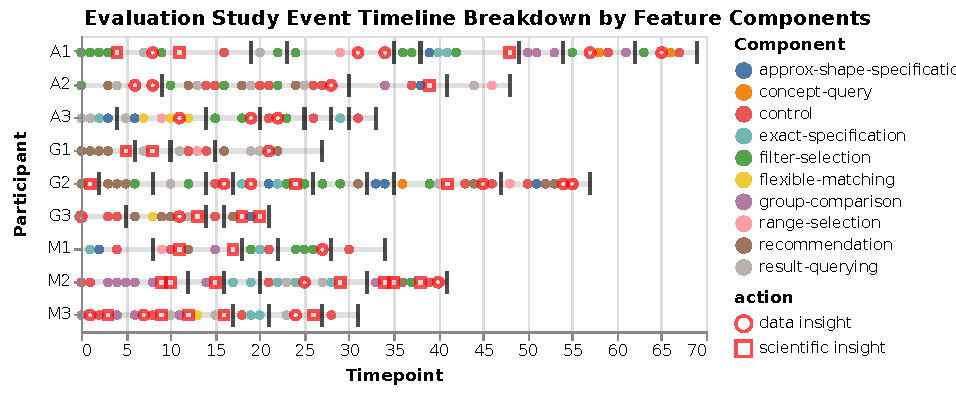
\includegraphics[width=\linewidth]{figures/evalstudytimeline.pdf}
%   \caption{Timeline of event code and component usage, with every timepoint as an event on the x axis. For clarity, we hide most of the event coding labels other than the insight labels. Black vertical tick indicates a session break, signaling the beginning of a new line of inquiry.}\label{fig:evalstudytimeline}
% \endminipage\hfill
% \minipage{0.4\textwidth}
%   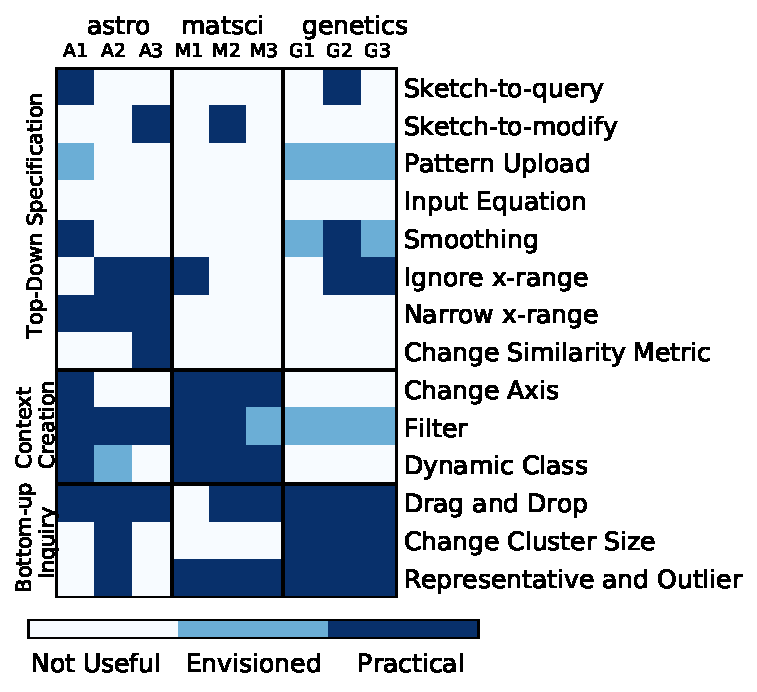
\includegraphics[width=0.8\linewidth]{figures/PENcoding.pdf}
%   \caption{Heatmap of features categorized as practical usage (P), envisioned usage (E), and not useful (N).  \techreport{We find that participants preferred to query using bottom-up methods such as drag-and-drop over top-down approaches such as sketching or input equations. Participants found that data faceting via filter constraints and dynamic class creation were powerful ways to compare between subgroups or filtered subsets. The columns are arranged in the order of subject areas and the features are arranged in the order of the three foraging acts.}}\label{fig:feature_heatmap}
% \endminipage
% \end{figure*}
Based on audio, video screen capture, 
and click-stream logs recorded 
during our evaluation study, 
we performed thematic analysis via open coding
and categorized every event with a coded label. 
Event codes included specific feature usage, 
insights, 
provoked actions, confusion, 
request for functionalities unaddressed 
by the system, and use of external tools.
% \begin{denselist}
%     \item Insight (Science): Insight that connected back to the science (e.g. ``This cluster resembles a repressed gene.'')
%     \item Insight (Data): Data-related insights (e.g. ``A bug in my data cleaning code generated this peak artifact.'')
%     \item Provoke (Science): Interactions or observations made while using the VQS that provoked a scientific hypothesis to be generated.
%     \item Provoke (Data): Interactions or observations made while using the VQS that provoked further data actions to continue the investigation.
%     \item Confusion: Participants were confused during this part of the analysis.
%     \item Want: Additional features that participant wants, which is not currently available on the system.
%     \item External Tools: The use of external tools outside of \zv to complement the analysis process.
% \end{denselist}
To characterize the usefulness 
of each feature, 
we further labeled whether each 
feature was useful to a particular participant's analysis. 
A feature was deemed \textit{useful} 
if the feature was either used in a sensible 
and meaningful way during the study, 
or has envisioned usage outside of the constrained 
time limit during the study 
(e.g., if data was available or downstream analysis was conducted). 
We derived these labels from the study transcript 
to circumvent self-reporting bias, 
which can often artificially inflate 
the usefulness of the feature under examination. 
\change{In this section, we will apply our thematic analysis results to understand how each sensemaking process occurs in practice.}%real-world analytic tasks.}
%\agp{Can't parse the previous sentence}
%categorized the features based on whether there was a sensible usage of the feature 
% into one of the three usage types based on how each feature was used during the study:
% \begin{denselist}
%     \item Practical: Features used in a sensible and meaningful way.
%     \item Envisioned: Features which could be used practically if the envisioned data was available or if they conducted downstream analysis, but was not performed due to the limited time during the study.
%     \item Not useful: Features that are not useful or do not make sense for the participant's research question and dataset.
% \end{denselist}
% \par Given these initial findings, we further investigated where the `sketch' 
% Our interactions with the scientists showed that different modalities for inputting a query can be useful for different problem contexts. In addition, the three paradigms of sensemaking described earlier are not mutually exclusive. In fact, we find that participants often construct a central workflow focused on features from one of the main paradigms and interleave variations with the feature usage from the two other paradigms as they iterate on the analytic task. As shown in Figure~\ref{fig:usagefreqbysubject}, the central paradigm adopted by each use case is tightly coupled with characteristics of the analytic challenges presented by each subject area.
% interplay
% Next, we will describe some of the design principles (DP) based on our study findings.
%focus on understanding the design space of VQSs and highlight the takeaways of our study.%developing a process model and design guideline for insight formation in VQSs and divert our thematic analysis of how VQSs fit into the context of an analysis workflow to our technical report.% These observation inform our ----- search-browse paradigm
% \subsubsection{Discovery of Real-world insights}
% \par Our participants' original workflow often required them to compare between many visualizations manually through separate analysis and visualization steps. Three of the participants cited that this segmented analyze-then-visualize workflow was one of their chief bottlenecks. The cognitive overhead from the segmented workflow made them more hesitant to visualize the results of different parameters and data operations, as A2 noted:
% \begin{quote}
% The quick visualization is something that I could not do on my current framework. I could not query as fast as you do; I need to wait for it, plot, and then compare. Every time I plot, I need to define subplots for 12 visualizations, then its slower. That's the reason why I sometimes plot less, and I rely more on the statistics from the likelihood tests. Sometimes I plot less than I really should be doing.
% \end{quote}
% The ability to rapidly experiment with large numbers of hypotheses in real time is a crucial step in the agile creative process in helping analysts discover actionable insights~\cite{Shneiderman2007a}. Five out of nine participants discussed how the dynamic, interactive update of the visualization in \zv was the main advantage for using VQSs over their original workflow.
% \begin{figure}[h!]
%   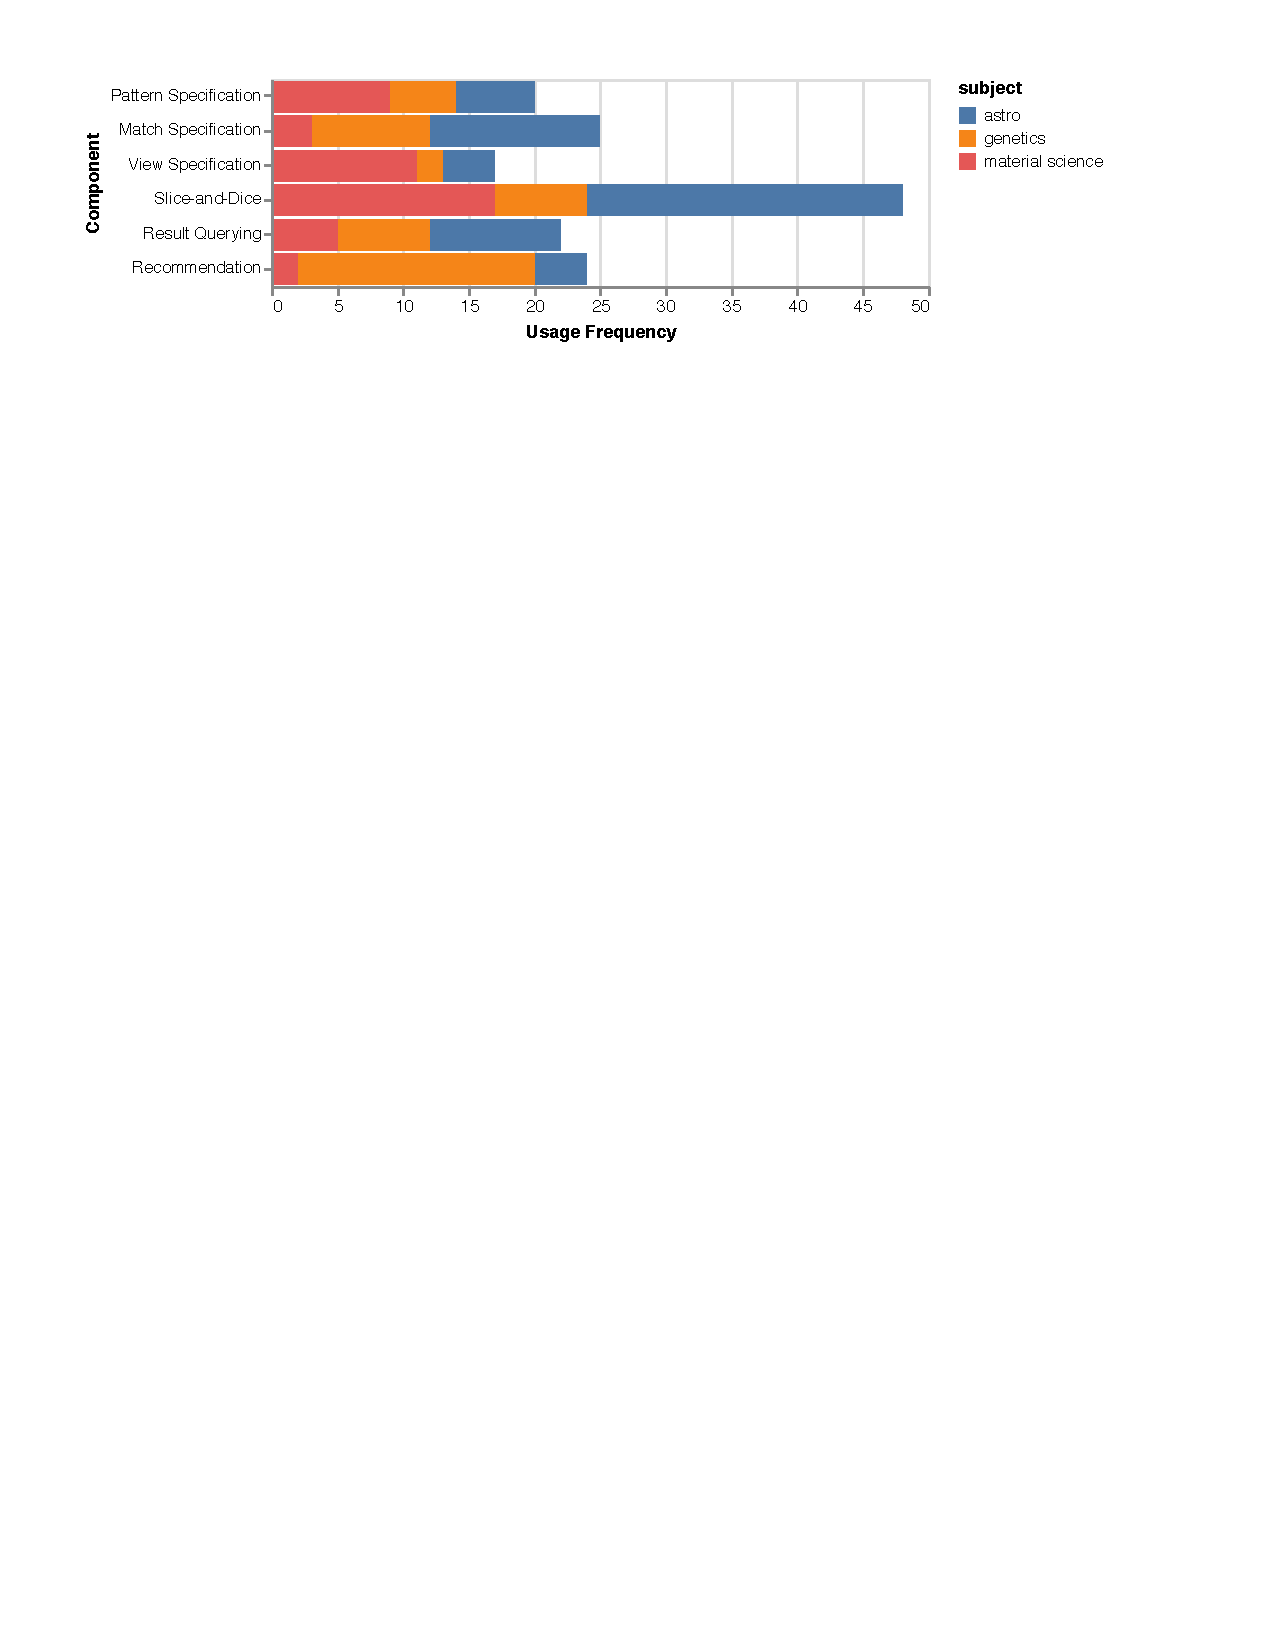
\includegraphics[width=\linewidth]{figures/usagefreqbysubject.pdf}
%   \caption{The number of times each component is used during the evaluation study, broken down by subject areas.}\label{fig:usagefreqbysubject}
% \end{figure}
\subsection{The Ineffectiveness of Sketch}
% \subsection{DC3: Closing the loop in VQS sense-making cycle with bottom-up data-driven inquries}
\par To our surprise, 
despite the prevalence of sketch-to-query 
systems in the literature, \techreport{Figure \ref{fig:feature_heatmap} shows that} only two out of our nine participants 
found it useful to directly
sketch their pattern onto the canvas (Figure~\ref{zvOverview}a). %Overall, bottom-up querying via drag-and-drop was more intuitive and more commonly used than top-down querying methods, such as sketching or input equations.
The main reason why participants 
did not find sketching that useful was that 
they often do not start their analysis with a specific pattern in mind. 
Instead, their intuition about what to query is derived
from other visualizations they encounter
during exploration, in which case it makes
more sense to query using those visualizations
as examples directly (e.g., by dragging and dropping
that visualization onto the sketch canvas via an action like
Figure~\ref{zvOverview}j). 
Even if a user has a pattern in mind,
translating that pattern into a sketch is often hard
to do. For example, 
A2 wanted to search for a highly-varying signal 
enveloped by a sinusoidal pattern indicating 
planetary rotation 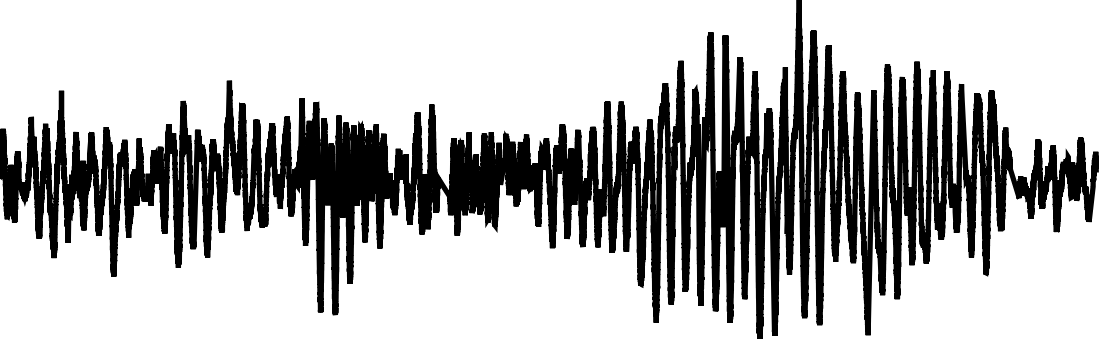
\includegraphics[width=2\baselineskip,keepaspectratio]{figures/impossible_sketch.png}, which is hard to draw by hand.
\begin{figure}[h!]
  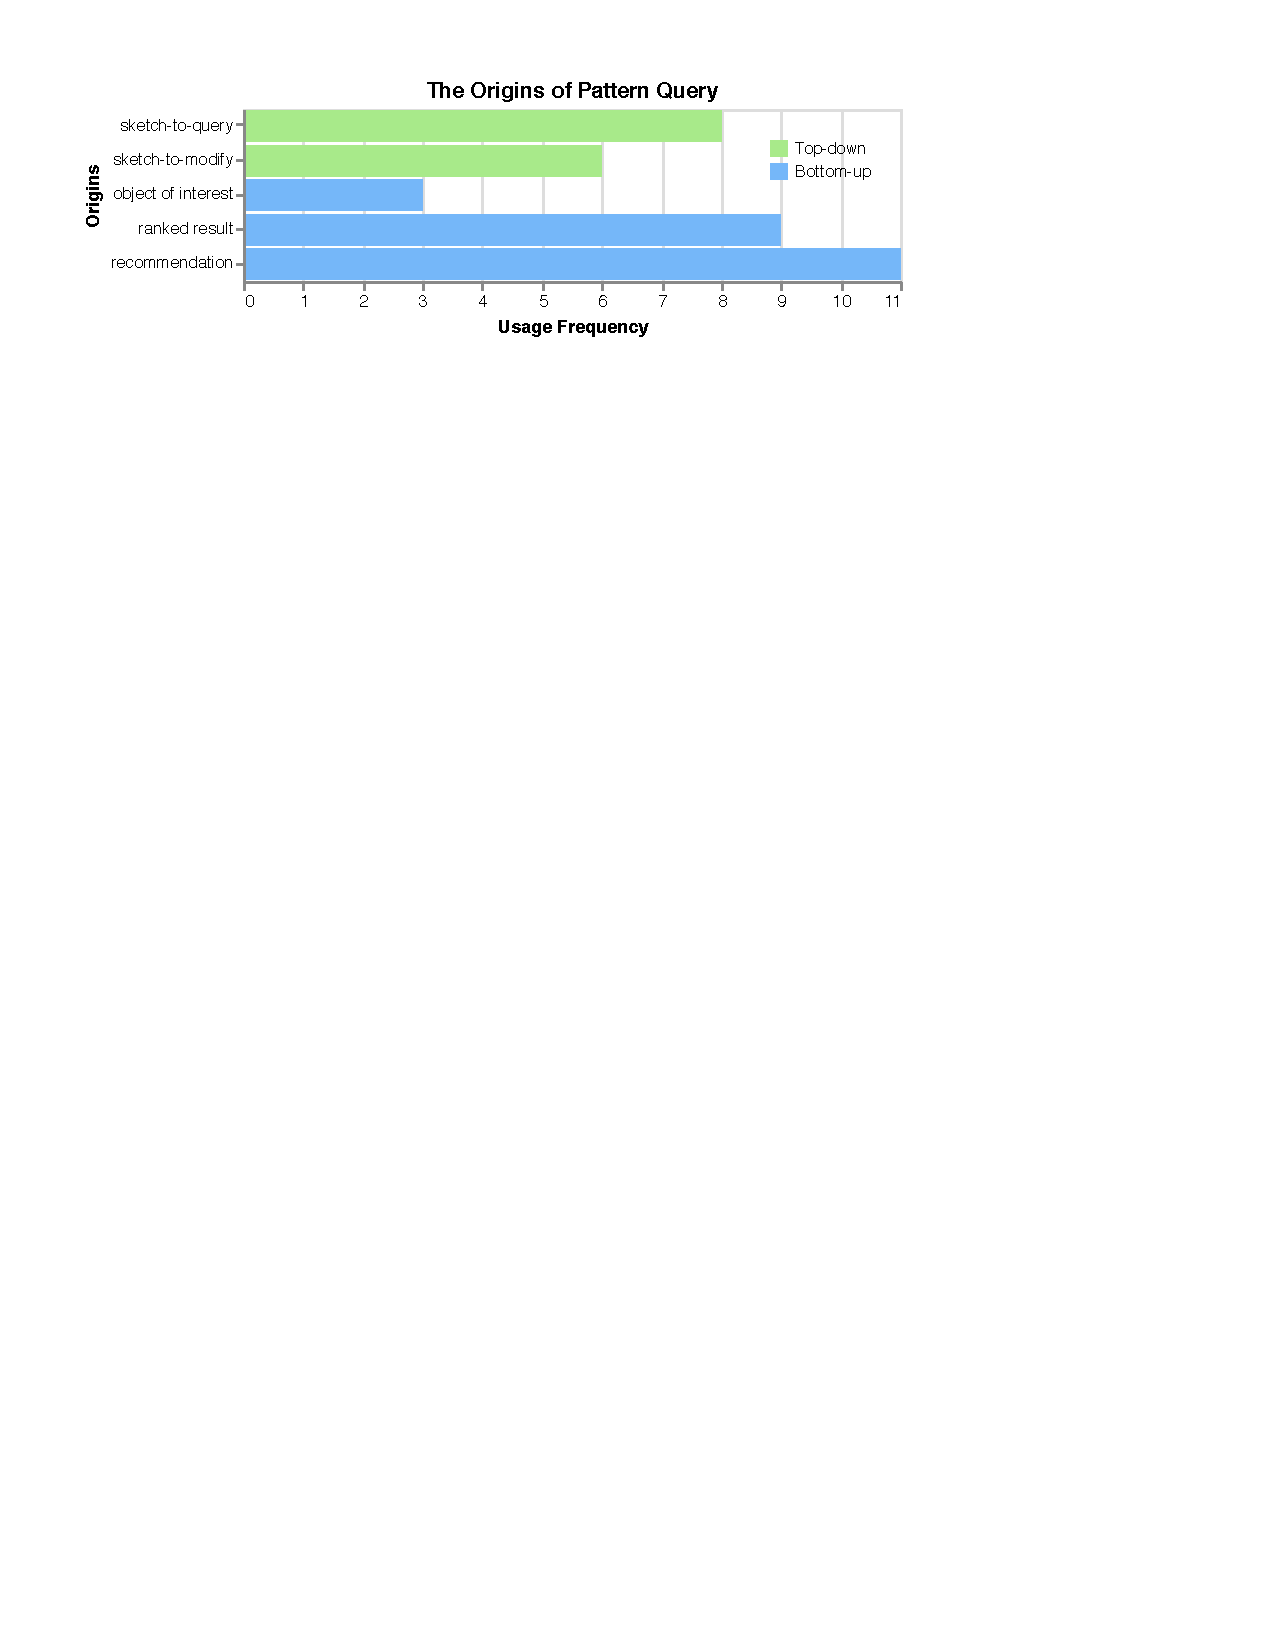
\includegraphics[width=\linewidth]{figures/the_origins_of_sketch.pdf}
  \vspace{-5pt}
  \caption{The number of times a pattern query originates from one of the workflows. We find that pattern queries are more commonly generated \change{via bottom-up than top-down processes.}}\label{fig:origins_of_sketch}
  \vspace{-5pt}
\end{figure}
\par Given these initial findings, 
we further investigated where the pattern 
on the canvas typically originates, \change{as presented in Figure~\ref{fig:origins_of_sketch}. 
Pattern queries can be generated by 
either top-down (sketching) or 
bottom-up (drag-and-drop) processes, 
driven by various different querying intentions. 
Within top-down processes, 
a pattern query could arise 
from users directly sketching 
a new pattern (sketch-to-query) 
or by modifying an existing sketch (sketch-to-modify).} % \agp{We don't really define what the various origins are clearly: what is sketch-to-query? what is sketch-to-modify?. Always describe what is going on in a figure clearly. I am left confused as I read through the rest. We shouldn't call it a sketch -- let's call it a pattern query. Delete the title from figure 5}
%Within these actions, there can be different intentions behind the sketch. While all visualizations that could be drag-and-dropped must come from the result or recommendation pane, a query can come from a particular object that the participant is interested in or simply through peripheral browsing of visualization results.%, described in the next section. 
%\par The latter case is also supported by the 
%\par There are also many unexpected use cases where sketching was simply used as a mechanism to modify an existing pattern query. 
For example, M2 first sketched a pattern 
to find solvent classes with anticorrelated 
properties without much success in returning a desired match.
%However, the sketched query did not return visualizations of interest.
So he instead dragged and dropped one 
of the peripheral visualizations similar 
to his desired visualization and then smoothed 
out the noise in the visualization yielding
a straight line, 
as shown in Figure \ref{query_modification} (left). 
M2 repeated this workflow twice in separate 
occurrences during the study and 
was able to derive insights from the results. 
Likewise, Figure~\ref{query_modification} (right) 
illustrates how A3 first picked out a regular pattern 
(suspected star spot), then modified it slightly 
so that the pattern looks more irregular (to find pulsating stars). %Likewise, A3 was interested in pulsating stars that looked similar to stellar hotspots in terms of its dramatic amplitude fluctuations, but differ in that their patterns exhibited irregularities. Figure \ref{query_modification} (right) showed how she first picked out a regular pattern (suspected star spot), then modified it slightly so that the pattern looks more irregular.
%Likewise, A3 was interested in pulsating stars characterized by dramatic changes in the amplitudes of the light curves. During the search, hotspots on stellar surfaces often show up as false positives as they also result in dramatic amplitude fluctuations, but happen at a regular intervals. In the VQS, A3 looked for patterns that exhibits amplitude variations, but also some irregularities. As shown in Figure \ref{query_modification} (right), she first picked out a regular pattern (suspected star spot), then modified it slightly so that the pattern looks more irregular.
\begin{figure}[h!]
    \centering
    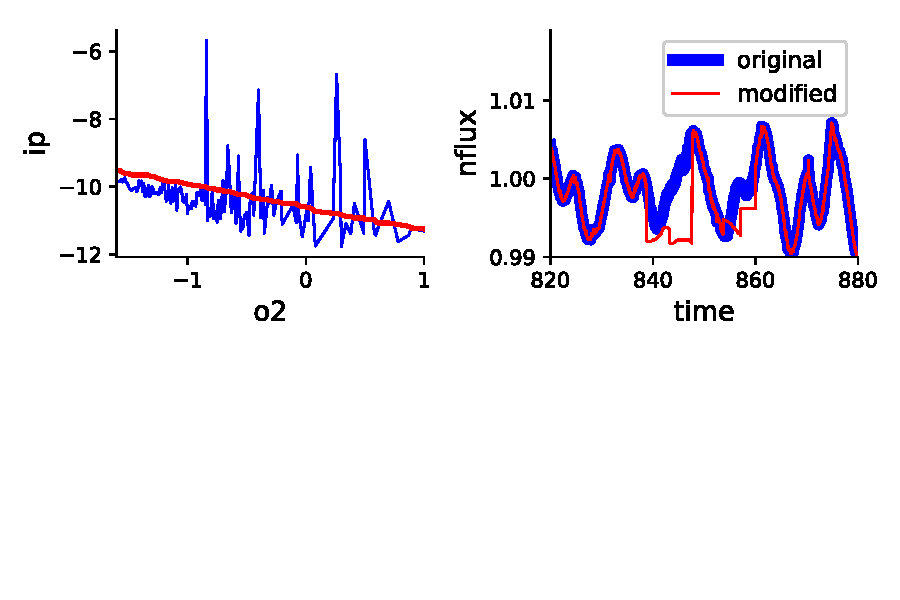
\includegraphics[width=\columnwidth]{figures/QueryModificationBySketch.pdf}
    \caption{Canvas traces from M2 (left) and A3 (right) during the study demonstrating query modification. The original drag-and-dropped query is shown in blue and the sketch-modified queries in red.}
    \label{query_modification}
    \vspace{-10pt}
\end{figure}
As described in the following section, 
bottom-up pattern queries can come from either 
the ranked list of results, 
recommendations, or by selecting a 
particular object of interest as a drag-and-drop query. 
Figure~\ref{fig:origins_of_sketch} shows that 
bottom-up processes are more common 
than top-down processes for generating a pattern query.

While all visualizations that could be drag-and-dropped 
must come from the result or recommendation pane, 
a query can come from a particular object 
that the participant is interested in or simply 
through peripheral browsing of visualization results.

\par The lack of practical use of top-down pattern 
specification is also reflected in the fact 
that none of the participants queried using an equation. 
In both astronomy and genetics, the visualization patterns 
resulting from complex physical processes 
that could not be written down as an equation analytically. 
Even in the case of material science when analytical 
relationships do exist, it is challenging to formulate 
functional forms in an prescriptive, ad-hoc manner.
% Despite functional fitting being common in scientific data analysis, Figure \ref{feature_heatmap} shows that
% . However,
\par These findings suggest that while sketching 
is an useful construct for people to express their queries, 
\emph{the existing ad-hoc, sketch-only model for VQSs 
is insufficient without data examples 
that can help analysts jumpstart their exploration}. 
In fact, from Figure~\ref{fig:origins_of_sketch},
we can see that sketch-to-query was used 
8 times, while the remaining modes were used 29 times altogether,
three times as much as sketch-to-query.
This finding has profound implications 
on the design of future VQSs, since Table~\ref{table:relatedwork} 
shows that past work have primarily focused 
on optimizing top-down process components, 
without considering how useful these features 
are in real-world analytic tasks.
%missing out largely on the key components in the other two paradigms \cut{(indicated by the absence of green features on the right hand side of the table)}.
We suspect that these limitations 
may be why existing VQSs are not commonly adopted in practice. %This result points to a need for ----- in future VQSs. %This, however, points to an exciting direction for sketching interface in VQSs for developing advanced drawing and modification tools that enable more precise visualization query specification.} %ed coverage in addressing different types of analytics use cases
%For instance, material science discovered a known inverse relationship during e xploration
%Which is really interesting. Which is something that we observed experimentally also. That is an interesting insight right htere. This seems to suggest that there is a fundamental issue in if you want to try to get better on this axis, and get as low as possible, you lose out on the other axis.
%once they see it they know it but they don't know beforehand

\subsection{Context Creation and Bottom-up Approaches}
\par As alluded to earlier, 
\emph{bottom-up data-driven inquiries 
and context creation are far more commonly 
used than top-down pattern specification 
when users have no desired patterns in mind}, 
which is typically the case for exploratory data analysis. 
In particular, we find that top-down approaches 
were only useful for 29\% of the use cases, 
whereas it was useful for 70\% of the use cases 
for bottom-up approaches and 67\% 
for context creation\change{\footnote{Feature usefulness is computed based on a matrix of usefulness labels for each use case (defined by a feature and user pair). The percentage of useful features for each process is computed as: $\frac{\textrm{\# of useful features in process}}{\textrm{total \# of features in process} \times \textrm{total \# of users}}$.}}.%number of features labeled as useful divided by the product of total number of features and total number of users}
%\agp{how did you get these stats? explain how you derived "useful for X\%"}. 
\change{We now highlight 
some of the exemplary workflows 
demonstrating the efficacy of the latter two sensemaking processes.}
%%The prevalence of bottom-up approaches not only point to the need for result querying, but also providing recommendations for users without desired patterns in mind.
\par As shown in Figure~\ref{fig:origins_of_sketch}, 
the most common use of bottom-up querying 
is via recommended visualizations. 
\change{For example, G2 and G3 identified that 
the three representative patterns 
recommended in \zvpp corresponded 
to the same three groups of genes discussed 
in a recent publication~\cite{Gloss2017}: 
induced genes (profiles with expression levels staying up), 
repressed genes (started high but went down), 
and transients (go up and then come down at different time points).}%Examples of how recommended trends can provoke further insightful actions comes from G2 and G3, who identified that the three representative patterns shown in \zvpp---induced genes (profiles with expression levels staying up), repressed genes (started high but went down), and transients (go up and then come down at different time points)---corresponded to the same three groups of genes discussed in a recent publication~\cite{Gloss2017}. 
The clusters provoked G2 to generate a hypothesis 
regarding the properties of transients: 
\textit{``Is that because all the transient groups 
get clustered together, or can I get sharp patterns 
that rise and ebb at different time points?''} 
To verify this hypothesis, G2 increased the parameter controlling the number of clusters and noticed that the clusters
no longer exhibited the clean, 
intuitive patterns he had seen earlier. 
G3 expressed a similar sentiment and proceeded 
by inspecting the visualizations 
in the cluster via drag-and-drop. 
He found a group of genes that all transitioned 
at the same timestep, while others transitioned 
at different timesteps. 
\techreport{G3 described the process of using 
VQSs as doing ``detective work'' that provoked 
him to generate further scientific hypotheses 
as well as data actions.} 
\par By browsing through the ranked list of 
results in \zvpp, participants were also able to 
gain a peripheral overview of the data 
and spot anomalies during exploration. 
For example, A1 spotted time series 
that were too faint to look like stars 
after applying the filter CLASS\_STAR=1, 
which led him to discover that all stars 
have been mislabeled with CLASS\_STAR=0 as 1 during data cleaning. 
%This includes inspecting the top-most similar visualizations that lie in the queried cluster. and finding visualizations that are similar to an object of interest that exhibits a desired pattern. %. After browsing through a series query results and checking with an external database, he concluded that 
 %We found that geneticists often gain their intuition about the data from the recommended representative trends. One example of rapid insight discovery
%the dataset had been incorrectly labelled with all the stars with CLASS\_STAR=0 as 1 during data cleaning.
\techreport{
	\begin{figure}[h!]
	  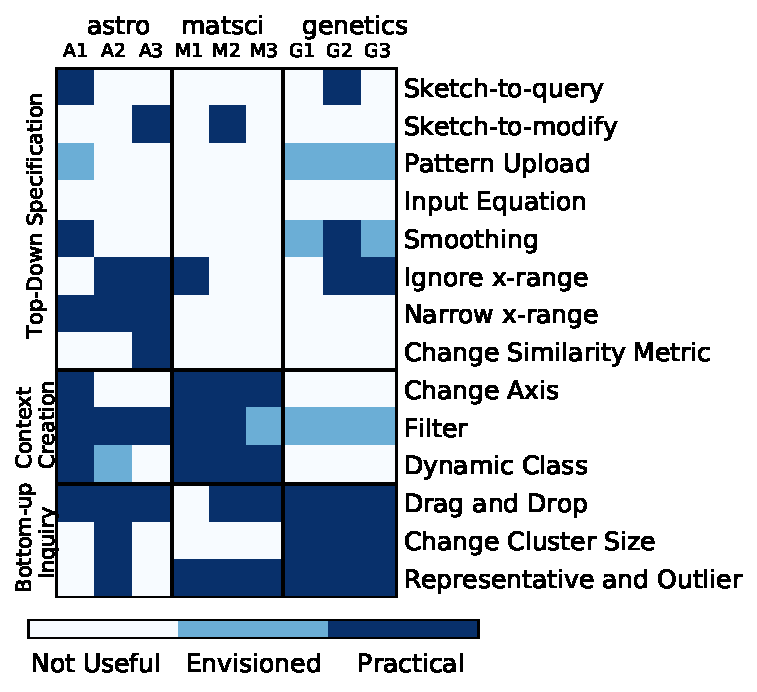
\includegraphics[width=0.8\linewidth]{figures/PENcoding.pdf}
	  \caption{Heatmap of features categorized as practical usage, envisioned usage, and not useful. \techreport{We find that participants preferred to query using bottom-up methods such as drag-and-drop over top-down approaches such as sketching or input equations. Participants found that slicing and dicing via filter constraints and dynamic class creation were powerful ways to compare between subgroups or filtered subsets. The columns are arranged in the order of subject areas and the features are arranged in the order of the three sensemaking processes.}}
	  \label{fig:feature_heatmap}
	\end{figure}
}
% \subsection{Enriching Search with Context}
\par Past studies in visual analytics 
have shown that it is important to design features 
that enable users to select relevant subsets of data~\cite{Amar2005,Heer2012}. 
Context creation in VQSs enables users to change the lens 
by which they look through the data 
when performing visual querying, 
thereby creating more opportunities 
to explore the data from different perspectives. 
All participants found at least 
one of the features in context creation to be useful.
%We designed two dynamic faceting features coupled with coordinated views that enabled users to specify subsets of data they are querying on and see immediate changes updated in the query, representative, and outlier results.
%either envisioned a use case or utilized features in the context creation paradigm to explore and compare subsets of their data.
%ven though the filtering step could be easily done with an external tool and reloaded into \zv, filtering on-the-fly was a powerful way to dynamically test his hypothesis. I
\par Both A1 and A2 expressed that 
interactive filtering enabled 
them to test conditions and tune values 
that they would not have otherwise modified, 
effectively lowering the barrier between 
the iterative hypothesize-then-compare cycle during sensemaking.
% echoing our previous finding that segmented workflow prevents extensive exploration.
During the study, participants used filtering 
to address questions such as: 
\textit{Are there more genes similar 
to a known activator when we subselect 
only the differentially expressed genes?} \techreport{\texttt{DIFFEXP=1} }(G2) or \textit{Can I find more supernovae candidates if I query only on objects that are bright and classified as a star?} \techreport{\texttt{flux\textgreater10 AND CLASS\_STAR=1} }(A1). Three participants had also used filtering as a way to pick out individual objects of interest to query with, as shown in Figure~\ref{fig:origins_of_sketch}. For example, G2 set the filter as gene=9687 and explained that since ``\textit{this gene is regulated by the estrogen receptor, when we search for other genes that resemble this gene, we can find other genes that are potentially affected by the same factors.}''
\par While filtering enabled users to 
narrow down to a selected data subset, 
dynamic class creation enabled users to compare 
relationships between multiple attributes and subgroups of data. 
For example, M2 divided solvents in the database 
into eight different categories based on voltage properties, 
state of matter, and viscosity levels, 
by dynamically setting the cutoff values 
on the quantitative variables to create these classes. 
By exploring these custom classes, M2 discovered that the relationship between viscosity and lithium solvation energy is independent of whether a solvent belongs to the class of high voltage or low voltage solvents and cited that dynamic class creation was central to learning about this previously-unknown attribute properties:
\begin{quote}
All this is really possible because of dynamic class creation, so this allows you to bucket your intuition and put that together. [...] I can now bucket things as high voltage stable, liquid stable, viscous, or not viscous and start doing this classification quickly and start to explore trends. [...] look how quickly we can do it!% Quite good!
\end{quote}
%Context creation is a useful ---- despite the --- pattern instance. Filtering still useful
%\par Participants employed \emph{a mix of bottom-up and top-down approaches when faceting through data in VQS}, including narrowing the search space based on some intuition about a phenomena, selecting individual visualizations, or specifying high-level groupings to compare and query with.
\subsection{The Sensemaking Process in VQSs}
Given our observations so far as to 
how participants 
make use of each sensemaking process in practice, 
we further investigate the interplay 
between these sensemaking processes 
in the context of an analysis workflow. %interplay with each other dynamically i% - Bottom up and context creation much more common than top-down. Stats \%. Brief Examples of each (How they are used in practice). 
% - BUT All three process are equally important. 
% - participants can go from one to the next and there is no single progression (e.g. context --> bottom -up --> top-down). 
% - Both the PageRank score (how important/“central” is the state is to the analysis?), raw occurrence of each state (how frequently is a feature categorized as part of the state used?) and the normalized self-directed edge score (how much user stays in that state?) coincide with what each subject area focuses on.
% We first examine the popularity of each sensemaking process based on how frequently they are used in the study. Figure~\ref{fig:feature_heatmap} show that features categorized as bottom-up (useful for 70\% of the use cases) and context creation (67\%) are much more useful compared top-down features (29\%). [Examples of Bottom up]. [Examples of Context Creation]. 
%Despite differing in levels of usage, each sensemaking process fulfills a central role in participants' analysis. 
% illustrates the state transitions computed based on event sequences from the evaluation study. %stay in the same state.
The event sequences from the evaluation study 
consist of labels describing when specific features were used. 
Using the taxonomy in Figure~\ref{fig:taxonomy}, 
we map each usage of a feature 
to one of the three sensemaking processes. 
Each participant's event sequence 
is divided into sessions, 
each indicating a separate lines of inquiry 
during the analysis. 
Based on these event sequences---one for each session, 
we compute the aggregate state transition probabilities 
(shown as edge weights in Figure~\ref{fig:transition}) 
to characterize how participants from each domain 
move between different sensemaking processes. 
For example, in material science, 
bottom-up exploration 
leads to context creation 60\% of the time 
and to top-down pattern-specification 
the rest of the time. 
Self-directed edges indicate the probability that the participant 
would continue with the same type of sensemaking process. 
For example, when an astronomer performs top-down pattern specification, 
it is followed by another top-down specification 
64\% of the time and context creation the rest of the time, 
but never followed by a bottom-up processes. 
This high self-directed transition probability 
reflects how astronomers often need to iteratively 
refine their top-down query through pattern 
or match specification when looking for a specific pattern. %when A1 looks for supernovae, he needs to iteratively refine his top-down query through pattern or match specification interfaces. %He could also chose to refine ----- , control --- to issue the desired query.
%Each event sequence is separated by labeled session breaks signaling the beginning of a new line of inquiry. The  
\begin{figure}[h!]
  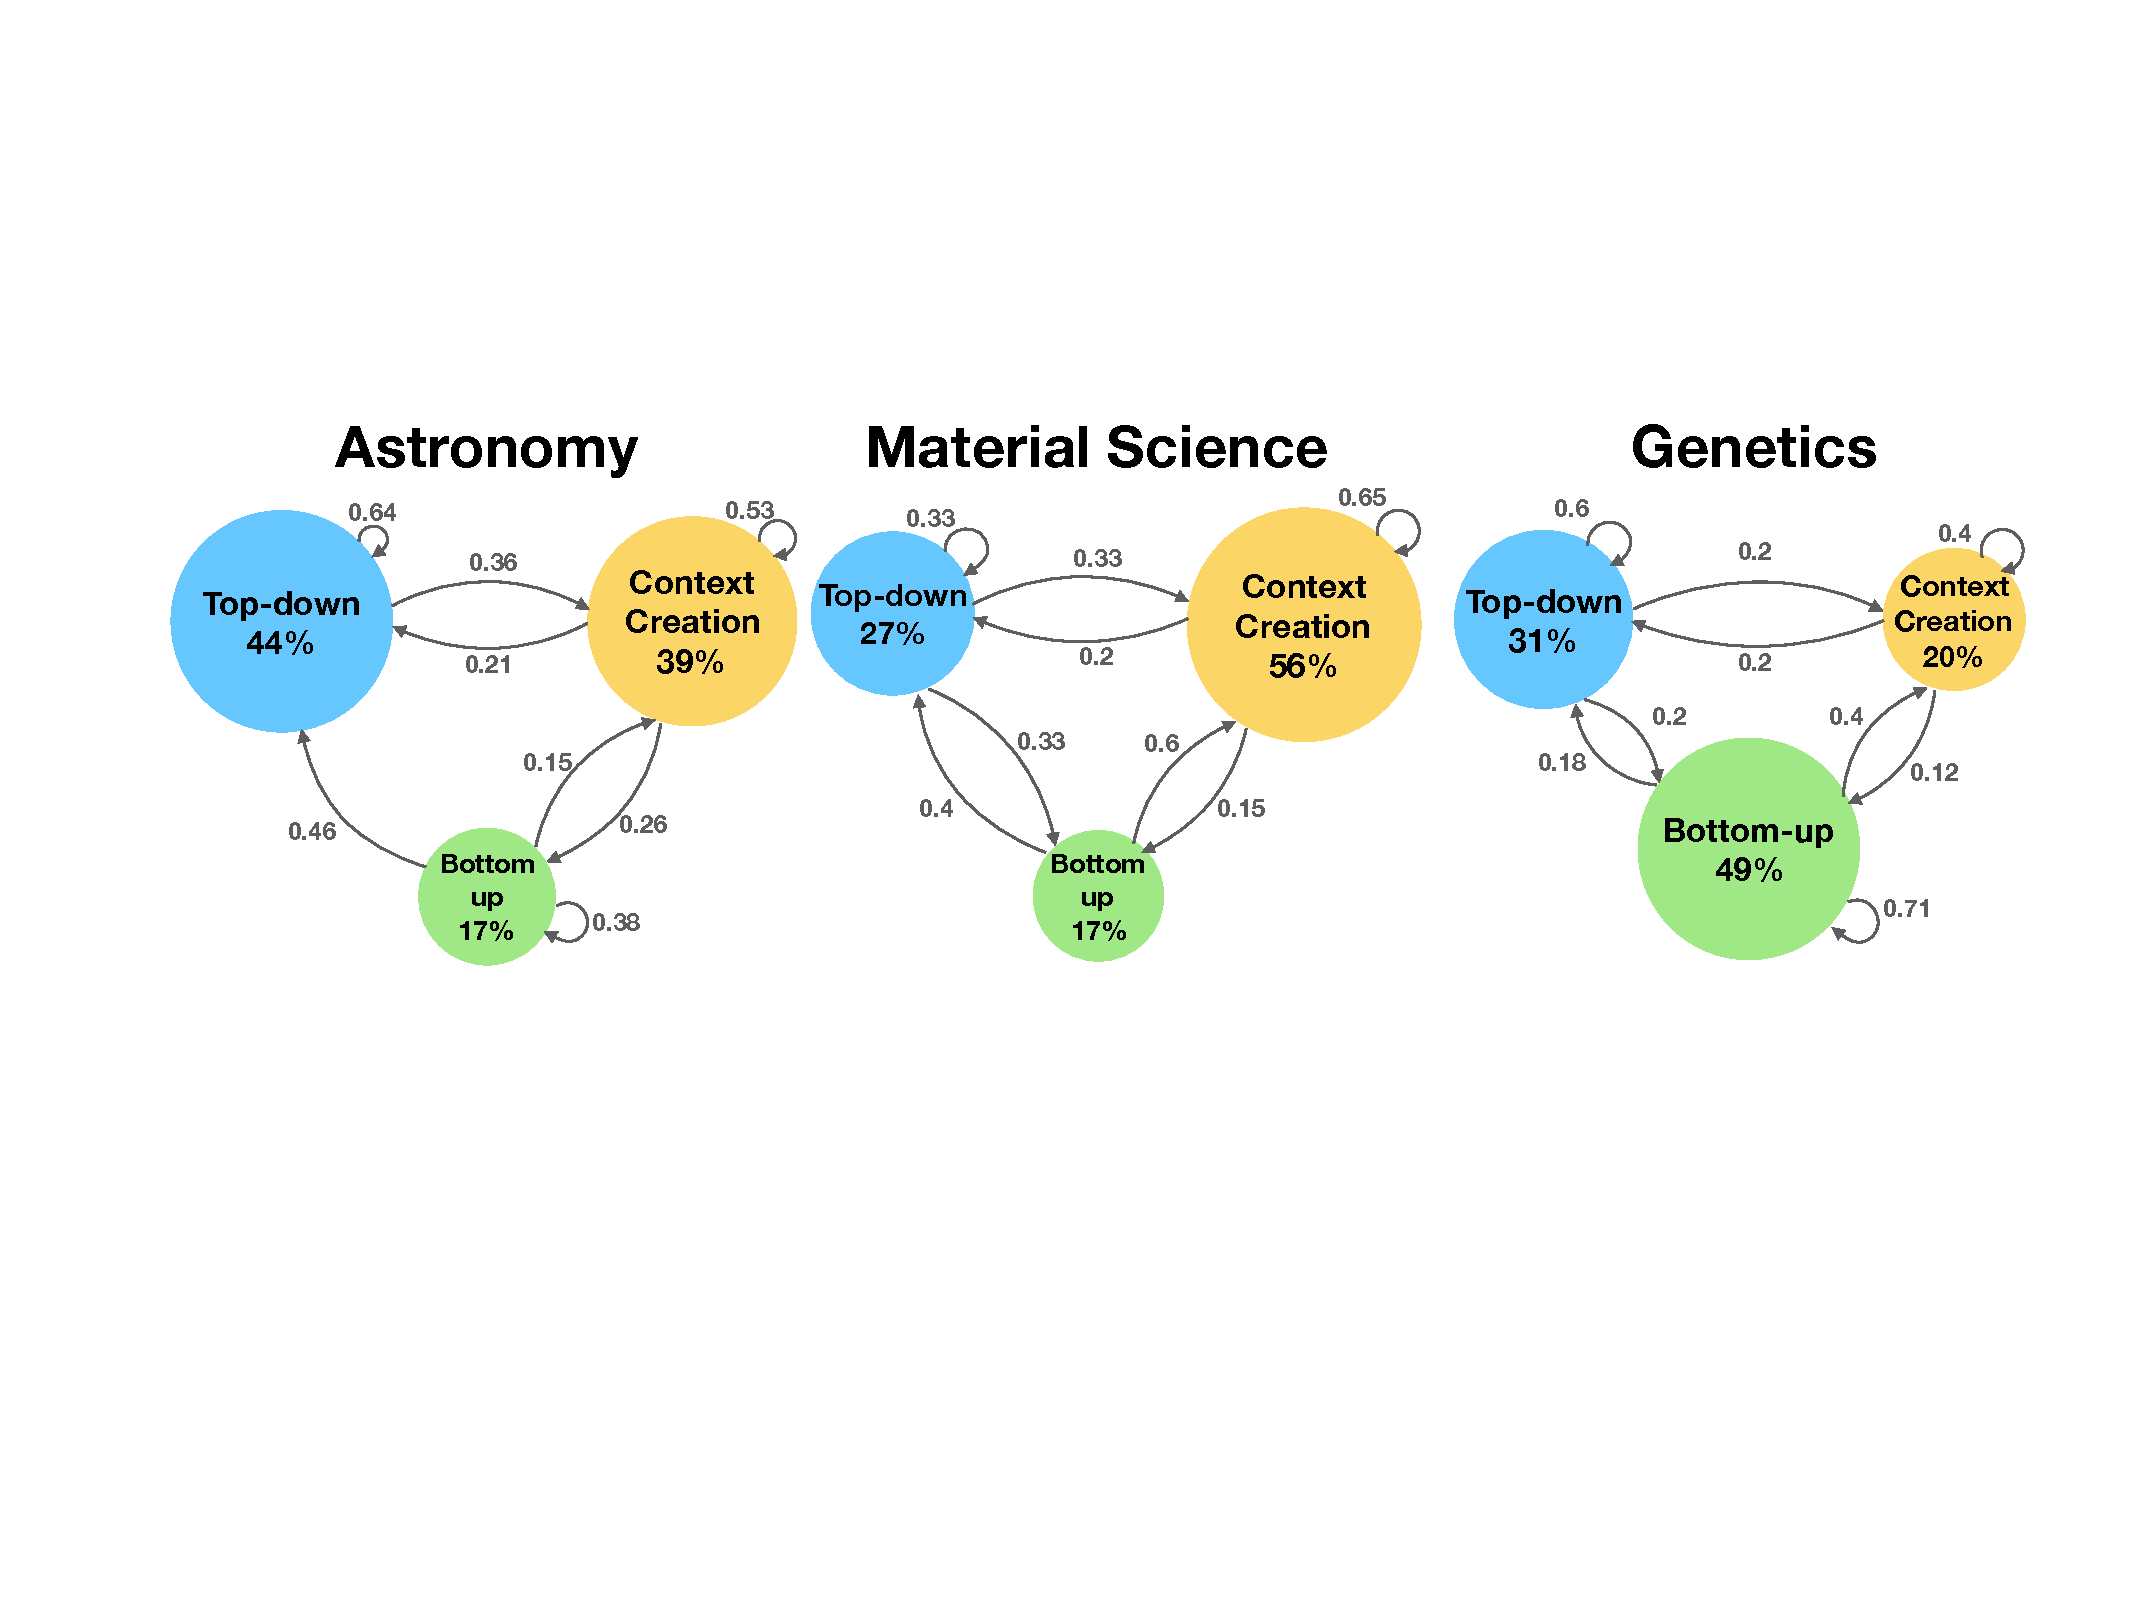
\includegraphics[width=\linewidth]{figures/markov_transition.pdf}
  \caption{Markov models computed based on the evaluation study event sequences, with edges denoting the probability that a participant in the particular domain will go from one sensemaking process to the next. Nodes are scaled according to the eigenvector centrality, which represents the percentage of time users spend in a particular state.}\label{fig:transition}
\end{figure}
% Similar to the sensemaking model proposed by Pirolli and Card~\cite{Pirolli}, the ---- sensemaking loop representing iterative process 
% ---- highlights how the two newly discovered VQS sensemaking process in this paper are essential for `closing the loop' between the sensemaking acts in VQSs. %, equally important  
% both the browsing-act through recommendations and performing search via these results are 
%These examples show that both the browsing-act through recommendations and performing search via these results are 
%The three sensemaking ----- not mutually exclusive, participants can go from one to the next and there is no single progression (e.g. context --> bottom -up --> top-down). Iterative blah blah. three process are equally important. 
%The three paradigms of sensemaking described earlier are not mutually exclusive. 
%Different sensemaking processes can be useful for different problem contexts.  
\par To study how important each sensemaking process 
is for participant's overall analysis, 
we compute the eigenvector centrality of each graph, 
displayed as node labels in Figure~\ref{fig:transition}. 
These values represent the percentage of time the participants
spend in each of the sensemaking processes 
when the transition model has evolved to a steady state. 
Given that nodes in Figure~\ref{fig:transition} 
are scaled by this value, in all domains, 
we observe that there is always a prominent node 
connected to two less prominent ones---but it is also clear
that all three nodes are essential to all domains.
Our observation demonstrates how participants 
often construct a central workflow 
around a main sensemaking process 
and interleave variations with the two other processes 
as they iterate on the analytic task. 
For example, material scientists focus 
on context creation 56\% of the time, 
mainly through dynamic class creation, 
followed by bottom-up inquiries (such as drag-and-drop)
 and top-down pattern specification (such as sketch modification). 
%through dynamic classes than top-down pattern specification. %astronomers focus largely on performing top-down pattern specification, while filtering on the visualization space.
The central process adopted by each domain 
is tightly coupled with characteristics 
of the analytic challenges associated with their subject area. 
For example, without an initial query in-the-head, 
geneticists relied heavily on bottom-up querying 
through recommendations to jumpstart their queries. 
%Despite the differing levels of usage from each subject area, we learn that \textit{each sensemaking process fulfills a central role in participants' analysis to address their high-level research objectives}.
% \agp{maybe point to figure?}.  
\par The transition model exemplifies how participants 
adopted a diverse set of workflows 
based on the unique set of research questions they brought to the study. 
The bi-directional and cyclical nature 
of the transition graph in Figure~\ref{fig:transition} highlights how the three sensemaking processes do not simply follow a linear progression, going from unknown to known pattern instance and visualized attributes in the problem space. Instead, the high connectivity of the transition model illustrates how these three equally-important processes form a sensemaking loop. The VQS sensemaking loop represents iterative acts of dynamic foraging and hypothesis generation. This flexibility is enabled by the diverse set of potential workflows that could be constructed in a full-fledged VQS like \zvpp, for addressing a wide range of analytical inquiries.%single-directional 
\subsection{Limitations}
\par Although evidence from our evaluation study 
suggests that direct sketch is inefficient, 
we have not performed controlled studies 
with a sketch-only system as a baseline to validate this hypothesis. 
The goal of our study is to uncover qualitative insights 
that might reveal why VQSs are not widely used in practice;
further validation of specific findings is out of the scope of this paper. 
While we have generalized our findings by employing 
three different and diverse domains (see Figure~\ref{fig:transition}), 
our case studies have so far 
been focused on scientific data analysis, 
as a first step towards greater adoption of VQSs. 
Other potential domains that could benefit from VQSs include: 
financial data for business intelligence, 
electronic medical records for healthcare, 
and personal data for ``Quantified Self''. 
These different domains may each pose different
 sets of challenges unaddressed 
 by the findings in this paper, 
 pointing to a promising direction for future work. 
% preliminary 
% While our results indicate that sketch is inefficient, we have not performed any controlled studies with sketch-only system as a baseline comparison to evaluate this hypothesis. support by evidence from our study
% - no A/B testing evaluate our hypothesis, direct comparison with a sketching. Our results points to an issue in this, further controlled studies required to validate these.
% , promising direction for future work.
% - study focussed on scientific workflow not BI or others --> towards social data , Quantified self
% - only 3 domain area breadth, but more than any existing work
%!TEX root = main.tex
\section{Conclusion\label{sec:conclusion}}
While VQSs hold tremendous promise in accelerating data exploration, they are rarely used in practice. In this paper, we worked closely with analysts from three diverse domains to characterize how VQSs can address their analytic challenges, collaboratively design VQS features, and evaluate how VQS functionalities are used in practice. Participants were able to use our final deployed system, \zvpp, for discovering desired patterns and trends, and obtaining valuable insights to address unanswered research questions. Grounded in these experiences, we developed a sensemaking model for how analysts make use of VQSs. Contrary to past work, we found that sketch-to-query is not as effective in practice as past work may suggest. Beyond sketching, we find that each sensemaking process fulfills a central role in participants' analysis workflows to address their high-level research objectives. We advocate that future VQSs should invest in understanding and supporting all three sensemaking processes to effectively `close the loop' in how analysts interact and perform sensemaking with VQSs. While more work certainly remains to be done, by contributing to a better understanding of how VQSs are used in practice across domains, our paper can also serve as a roadmap for broader adoption of VQSs,
and hopefully trigger exploration of novel use cases for these tools.
% the application of VQSs to ---- opportunities beyond ----
% for the broad adoption of VQSs in data analysis, opening up potential unexplored use cases and opprtunity for VQS. envision opportunities for VQSs beyond this to a larger space of use cases.
% process In discovering two ----- en ---opening up pathways  potential pathway worflow, while clo---- . 
% learn about the challenges they face when working with data. We extended our VQS \zv to the point where it could be effectively used for scientific data analysis. 
% Through participatory design, we identified three classes of missing interface capabilities  essential for employing VQSs for facilitating insight in real scientific applications, spanning expressive querying and dynamic faceting, as well as fine-grained control and understanding, along with the ability to compose flexible workflows in an integrated manner (RQ2). Finally, our evaluation study demonstrated how these features helped accelerate scientific insights (RQ3), as well as how they fit in the context of data analysis workflows (RQ4). One such finding is that bottom-up querying (e.g., drag-and-drop) is preferred over top-down (e.g., sketching) for exploratory data analysis, contrary to what is commonly supported in existing VQSs.
% point to focus on sci data but future work on quantified self and social viz
% VQS important 
% Our work : 
% - \zvpp
% - sensemaking model 
% domain problem characterization of visual querying through design studies with three different subject areas,
% \item abstraction of taxonomy and design space of VQSs grounded in participatory design findings,
% \item a full-fledge VQS, \zvpp, capable of facilitating rapid hypothesis generation and insight discovery,
% \item evaluation study findings regarding how VQSs are used in practice, leading to the formation of a novel sensemaking model for VQSs. %including the ineffectiveness of sketching and the ---- workflow  
% discover sketch 
% Our work closes the loop in VQS sensemaking so that VQS works in scenarios  where XY is unknown or Z is unknown. These areas were previously unexplored by past works.
% As presented in this section, our study is the first that contributes towards a holistic understanding of the sensemaking process for visual querying.
% ----- how they are used in practice. %Rather than assuming visual querying through sketch is useful, we 
% Our work is the first that evaluate on multiple case study participatory design, longitudinal study. 
% Participants intermixed functionalities across different sensemaking paradigms to address their problem contexts.
 % more thoroughly characterize the problem design space of VQSs and taxonomy abstraction for understanding the sensemaking process in VQSs. Moreover, we performed design studies with three different subject areas with a diverse set of questions, datasets, and challenges to further generalize our findings.
 % facilitating a diverse set of potential workflows and 
 % Both query by sketch and equations adopt a problematic assumption that analysts start with a known and easy-to-specify search pattern in mind. 
\newpage
\bibliographystyle{eg-alpha}
\bibliography{reference}
\newpage
\appendix
\section{Artifacts from Participatory Design\label{apdx:pdartifact}}
\begin{figure}[ht!]
	\centering
	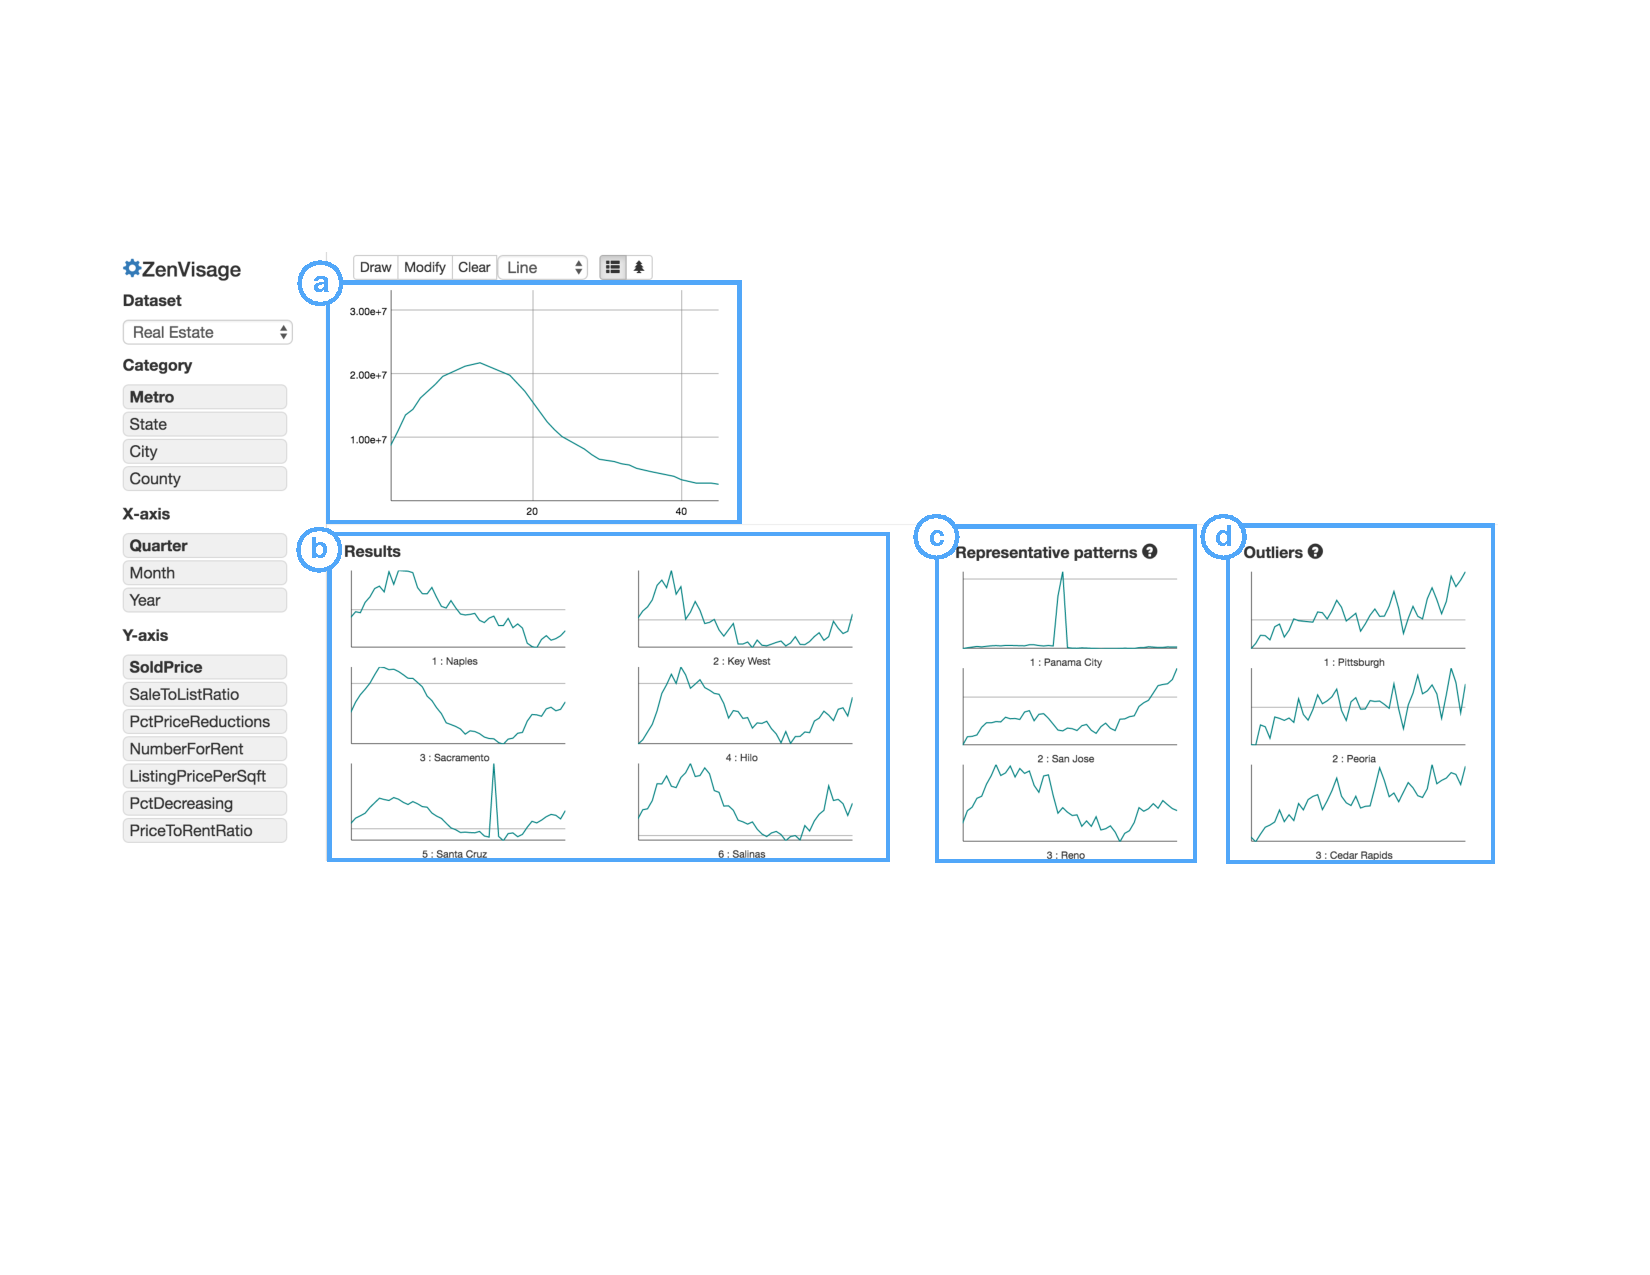
\includegraphics[width=\linewidth]{figures/oldZV_nozql.pdf}
	\caption{The existing \zv prototype allowed users to sketch a pattern in (a), which would then return (b) results that had the closest Euclidean distance from the sketched pattern. The system also displays (c) representative patterns obtained through K-Means clustering and (d) outlier patterns to help the users gain an overview of the dataset.}
	\label{oldZV}
	\end{figure}
\begin{figure}[!h]
  \centering
  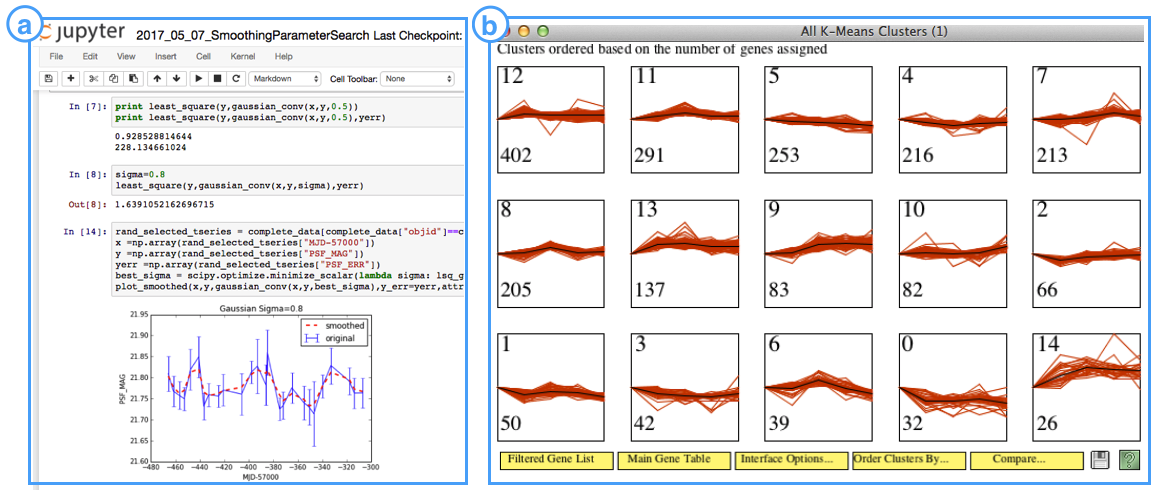
\includegraphics[width=\linewidth]{figures/workflow.png}
  \caption{Examples of the scientists' original workflow: a) The astronomer performs various data analysis task using the Jupyter notebook environment, b) The geneticists uses a domain-specific software to examine clustering outputs.}
  \label{workflow}
\end{figure}

\section{Evaluation Study Details\label{apdx:studydetails}}
We analyzed the transcriptions of the evaluation study recordings through open-coding and
categorized every event in the user study using the coding labels:
\begin{denselist}
    \item Insight (Science) \textbf{[IS]}: Insight that connected back to the science (e.g. ``This cluster resembles a repressed gene.'')
    \item Insight (Data) \textbf{[ID]}: Data-related insights (e.g. ``A bug in my data cleaning code generated this peak artifact.'')
    \item Provoke (Science) \textbf{[PS]}: Interactions or observations made while using the VQS that provoked a scientific hypothesis to be generated.
    \item Provoke (Data) \textbf{[PD]}: Interactions or observations made while using the VQS that provoked further data actions to continue the investigation.
    \item Confusion \textbf{[C]}: Participants were confused during this part of the analysis.
    \item Want \textbf{[W]}: Additional features that participant wants, which is not currently available on the system.
    \item External Tools \textbf{[E]}: The use of external tools outside of \zv to complement the analysis process.
\end{denselist}
\npar In addition, based on the usage of each feature during the user study, we categorized the features into one of the three usage types:
\begin{denselist}
    \item Practical usage \textbf{[P]}: Features used in a sensible and meaningful way.
    \item Envisioned usage \textbf{[E]}: Features which could be used practically if the envisioned data was available or if they conducted downstream analysis, but was not performed due to the limited time during the user study.
    \item Not useful \textbf{[N]}: Features that are not useful or do not make sense for the participant's research question and dataset.
\end{denselist}
The thematic encoding is summarized in Figure~\ref{feature_heatmap}.
\begin{figure}[ht!]
    \centering
    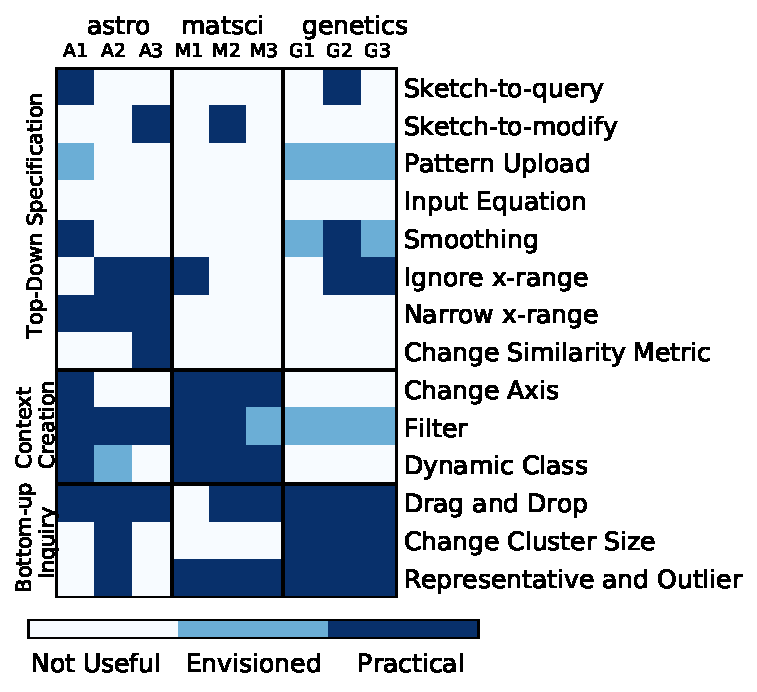
\includegraphics[width=0.7\columnwidth]{figures/PENcoding.pdf}
    \vspace{-6pt}\caption{Heatmap of features categorized as practical usage (P), envisioned usage (E), and not useful (N). We find that participants preferred to query using bottom-up methods such as drag-and-drop over top-down approaches such as sketching or input equations. Participants found that data faceting via filter constraints and dynamic class creation were powerful ways to compare between subgroups or filtered subsets. The columns are arranged in the order of subject areas and the features are arranged in the order of the three foraging acts.}
    \label{feature_heatmap}
    \vspace{-5pt}
\end{figure}
\dor{add event sequence based on codes.}

\end{document}
